\documentclass[anti,rapport,anglais]{note_technique_2018}

\newcommand\hmmax{0}
\newcommand\bmmax{0}

\titre{Hybrid High Order methods applied to incompressible
(visco-)plastic flows and phase field approaches of fracture.
Application de la méthode Hybrid High Order aux écoulements
(visco-)plastiques incompressibles et aux approches variationnelles de
la rupture.}

\titrecourt{Second year report of D. Siedel' PhD. Rapport de seconde
année de la thèse de D. Siedel.}

\input{LSC}

\auteurs{David Siedel, Thomas Helfer, Olivier Fandeur (*)}

\affiliation{(*) DES/ISAS/DM2S/SEMT/LM2S}

% \codebarre{img/barcode.jpg}

\redacteur{\mbox{D. Siedel}}

\fredacteur{\mbox{Doctorant}}

\verificateur{M. Josien (DEC/SESC/LM2C)}

% \dateversion{05/2021}

%\numero{21-005}

%\chrono{CEA/DES/IRESNE/DEC/SESC DO 54}

\indice{A}


\numeroaffaire{A-SICOM-02-01-01}

\clients{EDF-Framatome}

\domaine{SIMU}

\programmerecherche{SICOM}

\accords{CEA-EDF-FRAMATOME F35158}

\typeaction{80\% CEA -- 20\% EDF}

\usepackage{tcolorbox}
\usepackage[bbgreekl]{mathbbol}
\usepackage[eulergreek]{sansmath}
\usepackage{stmaryrd}

\newtcolorbox{myquote}{colback=blue!5!white, colframe=blue!75!black}
\renewenvironment{quote}{\begin{myquote}}{\end{myquote}}
\NoLogoAFAQ
\CoupeListeDiffusion
\diffusioninterne{%
DES/EC/DSE              & É. Proust           & 1 & Diffusion courriel\\
DES/EC/DPE/SIMU         & X. Raepsaet         & 1 & \\
                        & T. Laporte          & 1 & \\
DES/EC/DGCP/SA2P        & A. Soniak-Defresne  & 1 & \\
DES/ISAS/               & C. Santucci         & 1 & \\
                        & M. Serre            & 1 & \\
DES/ISAS/DMN            & P. Bossis           & 1 & \\
DES/ISAS/DPC/SECR/LECBA & B. Bary             & 1 & \\
DES/ISAS/DM2S           & P. Blanc-Tranchant  & 1 & \\
                        & D. Caruge           & 1 & \\
                        & E. Foerster         & 1 & \\
                        & G. Rampal           & 1 & \\
DES/ISAS/DM2S/STMF      & P. Gavoille         & 1 & \\
DES/ISAS/DM2S/STMF/LGLS & E. Adam             & 1 & \\
DES/ISAS/DM2S/SEMT      & S. Naury            & 1 & \\
                        & Y. Kaiser           & 1 & \\
DES/ISAS/DM2S/SEMT/LISN & C. Gourdin          & 1 & \\
DES/ISAS/DM2S/SEMT/DYN  & C. Gauthier         & 1 & \\
                        & B. Prabel           & 1 & \\
DES/ISAS/DM2S/SEMT/LM2S & J.-C. Le Pallec     & 1 & \\
                        & O. Fandeur          & 1 & \\
                        & F. Dipoala          & 1 & \\
IRESNE/DIR      & J-M. Morey & 1 &\\
                & C. Dellis & 1 &\\
                & P. Dumaz & 1 &\\
                & I. Tkatchenko & 1 &\\
DES/IRESNE/DEC          & M. Delpech   &   & Document disponible\\
                        & O. Charlent &   & sur intradec  \\
                        & C. Valot   &   & \\
DES/IRESNE/DEC/CP       & L. Sauvage     &   & \\
                        & É. Fédérici    &   & \\
DES/IRESNE/DEC/SESC     & M. Bauer       &   & \\
                        & R. Eschbach    &   & \\
DES/IRESNE/DEC/SESC/LEVA & A. Monnier    &   & \\
                          & J. Sercombe   &   & \\
DES/IRESNE/DEC/SESC/LECIM & N. Chikhi    &   & \\
DES/IRESNE/DEC/SESC/LM2C & E. Bourasseau &   & \\
DES/IRESNE/DEC/SESC/LSC & B. Collard     &   & \\
                        & V. Marelle     &   & \\
                        & T. Helfer      &   & \\
                        & D. Siedel      &   & \\
}


\diffusionexterne{%
EDF R\&D             & P. Barbrault    & 1 & Diffusion courriel \\
                     & C. Le Maître    & 1 & \\
EDF R\&D Palaiseau   & D. Geoffroy     & 1 & \\
                     & M. Abbas        & 1 & \\
                     & N. Pignet       & 1 & \\
EDF R\&D Renardières & R. Nhili        & 1 & \\
                     & Y. Sirsalane    & 1 & \\
                     & É. Pouillier    & 1 & \\
EDF/R\&D/CADARACHE   & K. Audic        & 1 & \\
                     & R. Largenton    & 1 & \\
                     & L. Parissi      & 1 & \\
                     & A. Kececioglu   & 1 & \\
EDF/DIPNN/DT         & J-J. Vermoyal   & 1 & \\
                     & P. Dias         & 1 & \\
                     & L. Barbié       & 1 & \\
EDF/DCN              & A.-F. Cotte     & 1 & \\
                     & R. Fernandes    & 1 & \\
                     & S. Pélissier    & 1 & \\
École Centrale Nantes/GEM        & N. Moès         & 1 & \\
UPMC/Institut d'Alembert & D. Leguillon & 1 & \\
INSA-Lyon/LAMCOS         & A. Gravouil  & 1 & \\
École des Ponts ParisTech/Laboratoire Navier         & J. Bleyer & 1 & \\
}


% Fix footnotes in tables (requires footnote package)

\usepackage{graphicx}

\resumeDO{

  This document describes two papers written during the second
  year of the PhD thesis of David Siedel:
  \begin{itemize}
    \item One deriving the Hybrid Discontinuous Galerkin (HDG)
    and Hybrid High Order (HHO) methods from the Hu-Washizu principle.
    \item One exploring a class of micromophorphic damage
    behaviours and their link with phase field approaches to fracture.
  \end{itemize}

  \textbf{Résumé français}

  Ce rapport décrit le travail réalisé au cours et autour de la
  seconde année du doctorat de D. Siedel. Ce travail s'est focalisé sur
  la rédaction de deux papier:

  \begin{itemize}
    \item L'un montrant comment les méthodes Hybrid
    Discontinuous Galerkin (HDG) et Hybrid High Order (HHO) peuvent être
    déduites du principe de Hu-Washizu.
    \item L'autre étudiant une classe de modèles micromorphes
    de l'endommagement et leurs liens avec les approaches par champs de
    phase.
  \end{itemize}
}

\resumeDR{
Sans objet.
}

\motsclefs{Méthode Hybrid High Order method. Approches variationnelles de
la rupture.}

\usepackage{amsmath}
\usepackage{amssymb}
\usepackage[euler]{textgreek}
\usepackage{soul}

\usepackage{graphicx}
\usepackage{../notations}

\newcommand*{\refname}{Bibliography}

\begin{document}

\chapter{Introduction}

This document describes two papers written during the second year of
the PhD thesis of David Siedel:
\begin{itemize}
  \item One deriving the Hybrid Discontinuous Galerkin (HDG) and
  Hybrid High Order (HHO) methods from the Hu-Washizu principle. This
  paper is reported in Chapter \ref{chapter:hho} of this report.
  \item One exploring a class of micromophorphic damage
  behaviours and their link with phase field approaches to fracture.
  This paper is reported in Chapter \ref{chapter:micromorphic_damage} of
  this report.
\end{itemize}

\chapter{Hybrid High Order methods for non-linear solid mechanics}
\label{chapter:hho}

\section{Introduction}
\label{sec_introduction}

\subsection{Outline}
\label{sec_introduction_outline}

% This paper aims at outlining a link between the Hu–Washizu
% variational principle and that of so called relaxed formulations
% % ,
% % from which are derived \textit{e.g.} Hybrid Discontinuous Galerkin
% % (HDG) methods, and, in particular, one of their latest refinement, the
% % Hybrid High Order (HHO) method.
% among which the family of Discontinuous Galerkin (DG) and Hybrid Discontinuous Galerkin
% (HDG) methods.
% This paper focuses on the specific case of Hybrid High Order (HHO) methods, that are a specific.
% , and, in particular, one of their latest refinement, the
% Hybrid High Order (HHO) method.

When solving quasi-incompressible boundary-value problems with the
Finite Element Method (FEM) using standard Lagrange interpolation, high
oscillations of the hydrostatic pressure might occur. This numerical
artifact, also known as volumetric locking is discussed in depth in
classical textbooks of computational
mechanics~\cite{simo_computational_1998, belytschko_nonlinear_nodate, neto_computational_2008}.
An enriched approach is required to resolve or, at least, alleviate
this issue.

Most works in the literature rely on either one of these two
following approaches to derive numerical methods robust to volumetric
locking:
\begin{itemize}
  \item The Hu-Washizu variational principle.
  \item Relaxed formulations, among which the family
  of Discontinuous Galerkin (DG) and Hybrid Discontinuous Galerkin (HDG)
  methods, including one of their latest refinement, the Hybrid High Order
  (HHO) method.
\end{itemize}

% Both these approaches introduce supplementary unknowns to the problem, and many works in the literature rely on either one of these two approaches to derive numerical methods that prove to be robust to volumetric locking phenomena.
% Both these methods are at the foundation of numerical methods

Both approaches introduce supplementary unknowns to the problem:
\begin{itemize}
  \item On the one hand, the Hu-Washizu variational principle
  extends that of Virtual Work by introducing supplementary stress and
  strain fields, that act as Lagrange multipliers to enforce
  respectively the constitutive and strain-displacement relations.
  \item On the other hand, relaxed formulations provide a richer
  kinematics by introducing a displacement jump at element boundaries,
  hence allowing for the definition of enhanced and local strain and
  stress fields.
\end{itemize}

The present paper proposes a variational formulation for HDG methods
based on a Hu-Washizu approach, where the discontinuity of the
displacement field is retrieved by introducing a linear elastic
interface between elements, hence outlining a common framework to both
Hu-Washizu based approaches for continuous displacement fields, and
hybrid discontinuous methods. A novel resolution algorithm, based on the
proposed variational approach is devised and numerically tested, using
the proposed HHO method for axi-symmetric problems.

% The following introduction outlines in a first part the development and applications of The Hu–Washizu variational
% formulation and in a second part that of discontinuous methods.

% DIRE HW A ETE REGARDE POUR LINCOMPRESSIBILITE PLASTIQUE ETC, AVANTDE PARLER DES LETHDODES
% -> INTRODUIRE LES 
% -> NOTATIONS (voir papier micromorphe)
% -> charges mortes pour les temres de passage en configurartion initiale, pas celles de Nanson
% -> les brackets : dimension finie, produit scalair intégrale, nsur des vectiueyrs : produit scalair vectoriel
% -> le potentiel élastique, non-standrad mais pour retrouver les expressions exactes des HDG, passer par vrai potentiel élastique , à tester. Passage en zone cohézive, extension intéressante pas traitée dans le document

% ---------------------------------------------------------
% -- SUBSECTION
% ---------------------------------------------------------
\subsection{From the Hellinger-Reissner principle to the Hu–Washizu variational formulation}

% Before 1950, variational principles considered only displacement
% as a single independent field.
% Generalized variational principles began in the 1950's with the
% breakthrough works of Reissner \cite{reissner_variational_1950} on two-field variational principles for elasticity problems, in
% which the displacement and stress were considered independent fields. Subsequently, de Vebeuke \cite{fraeijs_de_veubeke_diffusion_1951} constructed a
% four-field variational principle, and Hu \cite{hu_variational_1954} and Washizu \cite{washizu_variational_1955} established three-field variational
% principle independently.
% In 1983, Chien \cite{chien_method_1983} first pointed out that the three kinds of
% variables in Hu-Washizu principle are but nct independent
% of each other. Stress-strain relations are still its variational
% constraints, which could be removed only by high-order
% Lagrange multiplier method.

The principle of Virtual Work, which is at the foundation of the Finite Element theory, considers the displacement field alone as the unknown of the mechanical problem.
The first generalized variational principle dates back to the work of Reissner \cite{reissner_variational_1950} in the framework of linear elasticity, where the stress field does
not define as a function of the displacement gradient (or strain) anymore, but is now an unknown of the problem, in the same way as the displacement field.
In 1954 and 1955, Hu \cite{hu_variational_1954} and Washizu \cite{washizu_variational_1955} independently established a three-field variational principle, consisting of a stress,
a strain and a displacement field, hence giving rise to the so-called Hu-Washizu principle, which lays the groundwork for the so-called mixed and enhanced assumed strain methods.
However, de Vebeuke had already introduced in the early 50's a four-field principle, consisting of stress, strain, displacement and surface forces fields, and the Hu-Wahsizu principle
can be seen as an application of the de Vebeuke principle, where the surface force field is assimilated to the normal stress.

% ---------------------------------------------------------
% -- SUBSUBSECTION
% ---------------------------------------------------------
\paragraph{Assumed strain methods}

So-called Assumed Strain methods rely on an adaptation of the Hu-Washizu principle \cite{simo_variational_1985}, where a discrete interpolation of the strain is evaluated at the element level. Such a procedure allows,
following an appropriate choice in terms of discretization, to eliminate the stress and stress unknowns from the initial three field problem, resulting in the definition of a discrete differentiation operator,
which coined the name "Assumed strain". Among these methods is the famous "B-bar" method, that proves to be robust to volumetric locking.

% The denomination "assumed strain methods" is intended to encompass a variety of finite element procedures, often proposed on an ad-hoc basis, which are typically characterized by an interpolation of the discrete gradient operator assumed apriori, independently of the interpolation adopted for the displacement field. The often referred to "B-bar method", proposed by Hughes \cite{belytschko_ac0_1984}, offers an example of an assumed strain method which has proven successful in a variety of situations, including widely used structural elements \cite{hughes_finite_1981}.
% For the finite strain incompressible problem, this method has been precisely reformulated by Simo et al. \cite{simo_variational_1985} within the context of the Hu-Washizu principle.
% The so-called mode decomposition technique, proposed by Belytschko (e.g., [\textcolor{blue}{ref}]), furnishes another example of a B-bar type of method that leads to the formulation of successful structural elements.

% In XXX, Hughes and SImon showed that that assumed strain methods can be systematically formulated within the variational framework furnished by the Hu-Washizu principle. A crucial point in this development concerns the role played by the stress field, now entering the formulation as a Lagrange multiplier, and its recovery within the proposed variational structure. It is first noted that the Lagrange multipliers drop out from the formulation leading to a generalized displacement model, provided a certain orthogonality condition on the assumed strain field is satisfied. In addition, as a result of the variational structure, the admissible stress field (Lagrange multipliers) is constrained by an orthogonality condition arising from the Hu-Washizu principle as an Euler-Lagrange equation. These orthogonality conditions result in a single.

% ---------------------------------------------------------
% PARAGRAPH
% ---------------------------------------------------------
\paragraph{Mixed methods}

The term Mixed method denotes families of methods, that derive from the Hu-Washizu principle by introducing lower-order strain-based and stress-based tensorial fields
in place of the whole stress and strain fields. This can be done by introducing \textit{e.g.} a free energy potential split \cite{malkus_mixed_1978, al-akhrass_methodes_nodate}
(see Section \ref{sec_pressure_swelling} for more details on this note),
which allows to reduce the initial supplementary second order tensorial unknowns to \textit{e.g.} scalar pressure and swelling fields when considering incompressibility problems.

% Since volumetric locking is a pressure dependent phenomenon,
% considering for instance a decomposition of the stress and strain fields
% into \textit{e.g.} devatoric and spherical components, one can express a
% mixed problem in terms of pressure and swelling, which is at the origin
% of so-called UPG methods \cite{al_akhrass_integrating_2014,
%   simo_quasi-incompressible_1991,simo_variational_1985}. The scalar
% pressure and swelling unknowns replace respectively the stress and
% strain tensorial unknowns in \eqref{eq_HW_0} and a modified deformation
% gradient is introduced in the constitutive equation.

% In particular, Simo et al. \cite{simo_variational_1985} proved the equivalence of such an approach to that of the  Hu-Washizu principle when considering incompressibility problems.
% Studies concerning the equivalence of the modified displacement approaches and Hu-Washizu
% mixed approaches were conducted by Simo et al. \cite{simo_variational_1985} with regard to incompressibility problems. \cite{hughes_equivalence_1977,oden_observations_1975, shimodaira_equivalence_1985}

% At the same time,
% studies concerning the equivalence of the modified displacement approaches and Hu-Washizu
% mixed approaches were conducted by Simo et al. \cite{simo_variational_1985} with regard to incompressibility
% problems, and by Simo and Hughes \cite{simo_variational_1985} in a more general context of the assumed strain
% (B-bar) approach. Other related works are \cite{hughes_equivalence_1977,oden_observations_1975, shimodaira_equivalence_1985}

% ---------------------------------------------------------
% -- SUBSECTION
% ---------------------------------------------------------
\subsection{From Discontinuous Galerkin methods to Hybrid Discontinuous Galerkin methods}

% The Hybrid High Order method (HHO) is a discontinuous discretization
% method, that takes root in the Discontinuous Galerkin method (DG).
From the physical standpoint, discontinuous methods ensure the continuity of the flux
across interfaces, by seeking the solution element-wise, hence allowing
jumps of the potential across elements. They can be seen as a
generalization of Finite Volume methods, and are able to capture
physically relevant discontinuities without producing spurious
oscillations, such as volumetric locking.

% ---------------------------------------------------------
% -- SUBSUBSECTION
% ---------------------------------------------------------
\paragraph{Discontinuous Galerkin (DG) methods}

The origin of DG methods dates back to the pioneering work of
\cite{reed_triangular_1973}, where an hyperbolic formualtion is used to
solve the neutron transport equation. The first application of the
method to elliptic problems originates in \cite{babuska_finite_1973}
where Nitsche's method \cite{nitsche_uber_1970} is used to weakly impose
continuity of the flux across interfaces.
% ---> TODO : reformulate
In 2002, Hansbo and Larson \cite{hansbo_discontinuous_2002-1} were the first to
consider the Nitsche's classical DG method for nearly incompressible
elasticity. They showed, theoretically and numerically, that this
method is free from volumetric locking.
% --->

% % ---------------------------------------------------------
% % PARAGRAPH
% % ---------------------------------------------------------
% \paragraph{Application in Linear Elasticity}

%
%

% ---------------------------------------------------------
% PARAGRAPH
% ---------------------------------------------------------
\paragraph{Symmetric interior penalty}

Since the resulting bilinear form
arising from the initial formulation of DG methods is not symmetric, a so called interior
penalty term has been introduced in \cite{wheeler_elliptic_1978},
leading to the so-called Symmetric Interior Penalty (SIP) DG method. A first study
of the method to linear elasticity has been devised by
\cite{riviere_optimal_2000}, where optimal error estimate has been
proved.
%
%
%
% ---> TODO : reformulate
\cite{lew_optimal_2004} generalized the
Symmetric Interior Penalty method to linear elasticity.
In about the same
period of time, DG methods were proposed for other linear problems in
solid mechanics, such as Timoshenko beams
\cite{celiker_locking-free_2006}, Bernoulli-Euler beam and the
Poisson-Kirchhoff plate \cite{brenner_balancing_1999,
  engel_continuousdiscontinuous_2002} and Reissner-Mindlin plates
\cite{arnold_family_2005}. In the mid 2000's, the first applications
of DG methods to nonlinear elasticity problems was undertaken by
\cite{ten_eyck_discontinuous_2006, noels_general_2006}, and in 2007,
Ortner and Süli \cite{ortner_discontinuous_2007} carried out the a
priori error analysis of DG methods for nonlinear elasticity.
% --->

% % ---------------------------------------------------------
% % PARAGRAPH
% % ---------------------------------------------------------
% \paragraph{DG methods in solid mechanics}
% %
% %
% %
% DG methods then sollicitated a vigourus interest, mostly in fluid dynamics \cite{shahbazi_high-order_2007, persson_discontinuous_2009} due to their local conservative property and stability in convection domniated problems. However, except some applications for instance in fracture mechanics using XFEM methods \cite{gracie_blending_2008, shen_stability_2010}, or gradient plasticity \cite{djoko_discontinuous_2007,djoko_discontinuous_2007-1} DG methods did not break through in computational solid mechanics because of their numerical cost, since nodal unknowns need be duplicated to define local basis functions in each element.

% ---------------------------------------------------------
% -- SUBSUBSECTION
% ---------------------------------------------------------
\paragraph{Hybrid Discontinuous Galerkin (HDG) methods}

DG methods were then mostly deployed in fluid dynamics \cite{shahbazi_high-order_2007, persson_discontinuous_2009} due to their local conservative property and stability in convection dominated problems.
However, except some applications for instance in fracture mechanics using XFEM methods
\cite{gracie_blending_2008, shen_stability_2010}, or gradient plasticity \cite{djoko_discontinuous_2007,djoko_discontinuous_2007-1} DG methods did not break through in computational solid mechanics because of their numerical cost, since nodal unknowns need be duplicated to define local basis functions in each element.
To address this problem, in the early 2010's, \cite{cockburn_unified_2009, soon_hybridizable_2009} introduced additional faces unknowns on element interfaces for linear elastic problem, hence leading to the hybridization of DG methods, or Hybridizable Discontinuous Galerkin method (HDG). By adding supplementary boundary unknowns, the authors actually allowed to eliminate original cell unknowns by a static condensation process, in order to express the global problem on faces ones only.
% 
% % ---------------------------------------------------------
% % PARAGRAPH
% % ---------------------------------------------------------
% \paragraph{HDG methods in solid mechanics}
% 
Extension of HDG methods to non-linear elasticity were first undertaken in \cite{soon_hybridizable_2008} and have then fueled intense research works for various applications such as linear and non-linear convection-diffusion problems \cite{nguyen_implicit_2009,nguyen_implicit_2009-1,nguyen_hybridizable_2010}, incompressible Stokes flows \cite{nguyen_hybridizable_2010, nguyen_implicit_2011} and non-linear mechanics \cite{nguyen_hybridizable_2012}.

% ---------------------------------------------------------
% PARAGRAPH
% ---------------------------------------------------------
\paragraph{HHO methods}

In \cite{di_pietro_hybrid_2015, di_pietro_arbitrary-order_2014}, the authors introduced a higher order potential reconstruction operator in the classical HDG formulation for elliptic problems, providing a $h^{k+1} H^1$-norm convergence rate as compared to the usual $h^k$-rate. This higher order term coined the name for HHO methods.
Recent developments of HHO methods in
computational mechanics include the incompressible Stokes
equations (with possibly large irrotational forces) \cite{di_pietro_discontinuous_2016}, the
incompressible Navier–Stokes equations \cite{di_pietro_hybrid_2018}, Biot’s consolidation problem \cite{boffi_nonconforming_2016}, and nonlinear elasticity with small
deformations \cite{botti_hybrid_2017}

% \subsection{Aim of this paper}

% \subsection{Outline}

% In the first part of this paper, the Hu-Washizu variational principle is presented, and the Principle of Virtual Work is introduced as specification of the Hu-Washizu principle.
% The description of an element 
% ---------------------------------------------------------
% ---- SECTION
% ---------------------------------------------------------
\section{The standard Hu-Washizu variational approach}
\label{sec_model_problem}

This section introduces the standard Hu–Washizu three field
principle. For the sake of simplicity, and without loss of generality,
let consider the case of an hyperelastic material. Extensions to
mechanical behaviours with internal state variables are treated in
classical textbooks of computational mechanics
\cite{belytschko_nonlinear_nodate,besson_non-linear_2010}, and is outlined in Section \ref{sec:discretization:extension_to_non_linear_materials}
in the context of the proposed variational formulation for HDG methods.
% This extension in Section~\ref{sec:discretization:extension_to_non_linear_materials} for
% theorical aspects and in Section~\ref{sec_appendix_implementation} which
% discusses our numerical implementation of the Hybrid High Order method.
% This implementation is used in Section~\ref{sec_numerical_examples}
% which provides several examples in finite strain plasticity.

% ---------------------------------------------------------
% -- SUBSECTION
% ---------------------------------------------------------
\subsection{Description of the mechanical problem and notations}

% ---------------------------------------------------------
% PARAGRAPH
% ---------------------------------------------------------
\paragraph{Solid body}

Let us consider a solid body whose reference configuration is denoted
$\bodyLag$. At a given time $t > 0$, the body is in the current
configuration $\bodyEul$.

% ---------------------------------------------------------
% PARAGRAPH
% ---------------------------------------------------------
\paragraph{Mechanical loading}

The body $\bodyEul$ is assumed to be submitted to a body force $\loadEul$,
a prescribed displacement $\dirichletEul$ on the
Dirichlet boundary $\dirichletBoundaryEul$, and a surface load
$\neumannEul{}$ on the Neumann boundary $\neumannBoundaryEul$.

% ---------------------------------------------------------
% PARAGRAPH
% ---------------------------------------------------------
\paragraph{Deformation}

The transformation mapping 
$\tensori{\Phi}$ takes a point from the reference configuration $\bodyLag$ to the current
configuration $\bodyEul$ such that
%
%
%
\begin{equation}
    \tensori{\Phi}\paren{\tensori{X}} = \tensori{x} = \tensori{X}+\tensori{u}\paren{\tensori{X}}
\end{equation}
%
%
%
where $\tensori{X}$, $\tensori{x}$ and $\tensori{u}$ denote respectively
the position in the reference configuration $\bodyLag$, the position
in the current configuration $\bodyEul$ and the displacement.

% ---------------------------------------------------------
% PARAGRAPH
% ---------------------------------------------------------
\paragraph{Deformation gradient, gradient of the displacement}

The transformation gradient $\tensorii{F}$ is defined as
%
%
%
\begin{equation}
    \tensorii{F} = \nabla \tensori{\Phi} = \tensorii{I} + \tensorii{G}
\end{equation}
%
%
%
where $\nabla$ is the gradient operator in the
reference configuration and 
%
%
%
\begin{equation}
    \label{eq_grad_def}
    \tensorii{G} = \nabla \tensori{u}
\end{equation}
%
%
%
denotes the gradient of the
displacement.

% ---------------------------------------------------------
% PARAGRAPH
% ---------------------------------------------------------
\paragraph{Stress tensor}

The body is assumed made of an hyperelastic material described by a
free energy $\mecPotential_{\bodyLag{}}$ which relates the deformation gradient
$\tensorii{F}$ and the first Piola-Kirchhoff stress tensor $\tensorii{P}$ such that
%
%
%
\begin{equation}
    \label{eq_stress_def}
  \tensorii{P}=\deriv{\mecPotential_{\bodyLag{}}}{\tensorii{F}}
\end{equation}

% ---------------------------------------------------------
% PARAGRAPH
% ---------------------------------------------------------
\paragraph{Mechanical loading in the reference configuration}

$\bodyLag$ morphs under the action of volumetric forces $\tensori{f}_{V}$ and tractions forces
$\neumannLag$, that have been obtained from
their counterparts $\tensori{f}_{v}$ and $\neumannEul$ using the
Nanson formulae. In the following, for simplicity and without loss of generality,
they are assumed independent on the transformation gradient.
A prescribed displacement $\dirichletLag$ is imposed on $\dirichletBoundaryLag{}$.

% ---------------------------------------------------------
% -- SUBSECTION
% ---------------------------------------------------------
\subsection{Primal problem and principle of Virtual Work}

% ---------------------------------------------------------
% PARAGRAPH
% ---------------------------------------------------------
\paragraph{Total lagrangian}

The total Lagrangian $L^{VW}_{\bodyLag{}}$ of the body is defined as
the stored energy minus the work of external loadings, as follows:
%
%
%
\begin{equation}
\label{eq_Lagrangian}
L^{VW}_{\bodyLag{}}
% \paren{\tensori{u}}
= \int_{\Omega}\mecPotential_{\bodyLag{}}
(\tensorii{F}(\tensori{u}))
% (\tensorii{I} + \nabla \tensori{u})
% \paren{\tensorii{F}\paren{\tensori{u}}}
- \int_{\bodyLag} \tensori{f}{}_V \cdot \tensori{u}{}
- \int_{\neumannBoundaryLag} \neumannLag{} \cdot \tensori{u}{}
\vert_{\neumannBoundaryLag}
\end{equation}
%
%
%
% where the body forces $\tensori{f}_{V}$ and conctat tractions
% $\neumannLag$ in the reference configuration have been obtained from
% their counterparts $\tensori{f}_{v}$ and $\neumannEul$ using the
% Nanson formulae,
% and where the displacement field is prescribed by $\dirichletLag$ on $\dirichletBoundaryLag{}$ in the reference configuration.
% In the following, for simplicity and without loss of generality,
% Dirichlet boundary conditions are omitted from the developments, and volumetric and surface loads are assumed independent on the transformation gradient.
% 
% % ---------------------------------------------------------
% % PARAGRAPH
% % ---------------------------------------------------------
% \paragraph{Principle of Virtual Works}
% 
The displacement $\tensori{u}$ satisfying
the mechanical equilibrium minimizes the Lagragian $L^{VW}_{\bodyLag{}}$.
The first order variation of the Lagrangian is given by
%
%
%
\begin{equation}
  \label{eq_virtual_works_0}
  % \langle \frac{\partial L^{VW}_{\bodyLag{}}}{\partial \tensori{u}} \cdot \delta \tensori{u} \rangle
  \langle \frac{\partial L^{VW}_{\bodyLag{}}}{\partial \tensori{u}} , \delta \tensori{u} \rangle
  =
  \int_{\bodyLag} \tensorii{P} : \nabla \delta \tensori{u} -
  \int_{\bodyLag} \tensori{f}_V \cdot \delta \tensori{u} -
  \int_{\neumannBoundaryLag} \neumannLag{} \cdot \delta \tensori{u}
  \vert_{\neumannBoundaryLag}
\end{equation}
%
%
%
which must be null for the the solution displacement, and thus yields the well known principle of \textit{Virtual Work},
where the notation $\langle \cdot , \cdot \rangle$ defines the usual duality pairing.
% where the left-hand side of \eqref{eq_virtual_works_0} reads as the well known \textit{Principle of Virtual Work}.
% . The solution
% displacement thus satisfies the principle of virtual work
% %
% %
% %
% \[
% \int_{\bodyLag} \tensorii{P} : \nabla \delta \tensori{u} =
% \int_{\bodyLag} \tensori{f}_V \cdot \delta \tensori{u} +
% \int_{\neumannBoundaryLag} \neumannLag{} \cdot \delta \tensori{u}
% \vert_{\neumannBoundaryLag}
% \quad
% \forall \delta \tensori{u}{}
% \]

% ---------------------------------------------------------
% -- SUBSECTION
% ---------------------------------------------------------
\subsection{The Hu-Washizu variational approach}
\label{sec_HW_lagrangian}

\paragraph{Hu-Washizu Lagrangian}

The Hu-Washizu Lagrangian $L^{HW}_{\bodyLag{}}$
\cite{hu_variational_1954, washizu_variational_1955, washizu_variational_1974} generalizes
the previous variational principle by considering that the gradient of
the displacement $\tensorii{G}$ and the first Piola-Kirchoff
$\tensorii{P}$ stress are independent unknowns of the problem, such
that:
%
%
%
\begin{equation}
  \label{eq_HW_0} L^{HW}_{\bodyLag{}}
  % \paren{\tensori{u},\tensorii{G}, \tensorii{P}}
  = \int_{\bodyLag{}}
  \mecPotential_{\bodyLag{}}
  % (\tensorii{I}+\tensorii{G})
  (\tensorii{F}(\tensorii{G}))
  + \int_{\bodyLag{}}  (\nabla
  \tensori{u}{} - \tensorii{G}{})\,\colon\,\tensorii{P} -
  \int_{\bodyLag{}} \loadLag \cdot \tensori{u}{} -
  \int_{\neumannBoundaryLag{}} \neumannLag{} \cdot \tensori{u}
  \vert_{\neumannBoundaryLag}
\end{equation}
%
%
%
The solution $(\tensori{u}, \tensorii{G}, \tensorii{P})$
satisfying the mechanical equilibrium minimizes the Lagragian
$L^{HW}_{\bodyLag{}}$. The first order variation of the Hu-Washizu
Lagragian with respect to $\tensori{u}, \tensorii{G}$, and
$\tensorii{P}$ yields % % %
\begin{subequations}
  \label{eq_hu_washizu_derivative_0}
  \begin{alignat}{3}
    \langle \frac{\partial L^{HW}_{\bodyLag{}}}{\partial \tensori{u}} , \delta \tensori{u} \rangle
    =
    % \deriv{L^{HW}_{\bodyLag{}}}{\tensori{u}}
    % \cdot \delta \tensori{u}
    % =
    & \int_{\bodyLag} \tensorii{P} : \nabla
    \delta \tensori{u} - \int_{\bodyLag} \tensori{f}_V \cdot \delta
    \tensori{u} - \int_{\neumannBoundaryLag} \neumannLag \cdot \delta
    \tensori{u} \vert_{\neumannBoundaryLag} && \ \ \ \ \ \ \ \ &&
    \forall \delta \tensori{u}{} \label{eq_hu_washizu_derivative_0:eq0}
    \\
    \langle \frac{\partial L^{HW}_{\bodyLag{}}}{\partial \tensorii{P}} , \delta \tensorii{P} \rangle
    % \deriv{L^{HW}_{\bodyLag{}}}{\tensorii{P}}
    % : \delta \tensorii{P}
    =
    & \int_{\bodyLag} ( \nabla \tensori{u} -
    \tensorii{G} ) : \delta \tensorii{P} && \ \ \ \ \ \ \ \ && \forall
    \delta \tensorii{P}{} \label{eq_hu_washizu_derivative_0:eq2}
    \\
    \langle \frac{\partial L^{HW}_{\bodyLag{}}}{\partial \tensorii{G}} , \delta \tensorii{G} \rangle
    % \deriv{L^{HW}_{\bodyLag{}}}{\tensorii{G}}
    % : \delta \tensorii{G}
    = & \int_{\bodyLag} (\frac{\partial
      \mecPotential}{\partial \tensorii{G}} - \tensorii{P}) : \delta
    \tensorii{G} && \ \ \ \ \ \ \ \ && \forall \delta \tensorii{G}{}
    \label{eq_hu_washizu_derivative_0:eq3}
  \end{alignat}
\end{subequations}
where Equations~\eqref{eq_hu_washizu_derivative_0:eq2}
and~\eqref{eq_hu_washizu_derivative_0:eq3} account
for~\eqref{eq_grad_def} and~\eqref{eq_stress_def} respectively in a weak
sense.

% ---------------------------------------------------------
% -- SUBSECTION
% ---------------------------------------------------------
\subsection{Classical applications of the Hu-Washizu variational
  approach in computational mechanics to circumvent volumetric locking}

In the continuous framework, the Hu-Washizu functional is not
relevant, since Equations~\eqref{eq_hu_washizu_derivative_0:eq2}
and~\eqref{eq_hu_washizu_derivative_0:eq3} would lead to the following
equalities:
%
%
%
\begin{equation}
  \begin{aligned}
    \tensorii{G} = \nabla\tensori{u} && \text{and} && \tensorii{P}=\frac{\partial \mecPotential}{\partial \tensorii{G}}
  \end{aligned}
\end{equation}
%
%
%
% \[
% \tensorii{G} = \nabla\tensori{u}
% \quad\text{and}\quad
% \tensorii{P}=\frac{\partial \mecPotential}{\partial \tensorii{G}}
% \]
% 
However, considering finite-dimensional functional spaces, multiple choices arise
for the specification of the Lagrangian \eqref{eq_HW_0}.

% ---------------------------------------------------------
% PARAGRAPH
% ---------------------------------------------------------
\paragraph{Pressure swelling formulations}
\label{sec_pressure_swelling}

Since volumetric locking is a pressure dependent phenomenon,
considering for instance a decomposition of the stress and strain fields
into \textit{e.g.} devatoric and spherical components, one can express a
mixed problem in terms of pressure and swelling, which is at the origin
of so-called UPG methods \cite{al_akhrass_integrating_2014,
  simo_quasi-incompressible_1991, simo_variational_1985}. The scalar
pressure and swelling unknowns replace respectively the stress and
strain tensorial unknowns in \eqref{eq_HW_0} and a modified deformation
gradient is introduced in the constitutive equation.

% ---------------------------------------------------------
% -- SUBSECTION
% ---------------------------------------------------------
\paragraph{Enhanced assumed strains formulations}
\label{sec_eas}

Another approach of the use of the Hu-Washizu consists in
studying the equilibrium of a single element. Such a framework falls
into the scope of so-called Enhanced Assumed Strains methods
\cite{simo_variational_1986, simo_class_1990}, which result for instance
in the "B-bar" method.
It consists in eliminating both the stress and gradient field, by defining a discrete gradient operator
that verifies a certain orthogonality condition with the stress field,
such that the sole displacement unknowns remains in the formulation.
Such a procedure is somehow similar to the one described in Section \ref{sec_hdg_element_equilibrium},
where both the stress and gradient fields are also eliminated from the problem.

% ---------------------------------------------------------
% -- SUBSECTION
% ---------------------------------------------------------
\paragraph{Towards Discontinuous methods}

In the present document, an introduction to so-called
\textit{non-conformal} methods is proposed, by means of the Hu–Washizu Lagrangian.
At the origin of these methods is the Discontinuous Galerkin (DG)
method, which postulates the discontinuity of the displacement across
elements. This feature allows the method to be robust to volumetric
locking. However, its formulation takes root in a possibly dry
mathematical background, and the ingredients of the method are not
introduced in the literature through physical arguments. The
next section aims at introducing the whole framework of non-conformal
methods, including the displacement discontinuity, through the
Hu–Washizu Lagragian.
The main difference with former works using both a Hu-Washizu Lagrangian in the context of Discontinuous methods is that the present document
introduces the discontinuity of the displacement field from the application of the Hu-Washizu Lagrangian to an element surrounded by an interface as defined in Section \ref{sec_appendix_composite_demo},
whereas \textit{e.g.} \cite{noels_general_2006} and \cite{neunteufel_three-field_2021} formulate a Hu-Washizu Lagrangian using a discretization that already incorporates the discontinuity of the displacement field.
In particular, the proposed variational formulation in Section \ref{sec_hdg_element_equilibrium} naturally introduces the main ingredients of HDG methods (namely the \textit{reconstructed gradient} and the \textit{reconstructed traction force}) as a consequence of the minimization of some Lagrangian, instead of introducing them \textit{a priori}.

% Though one counts a few occurances of the use of the Hu–Washizu Lagragian in the context of discontinuous methods \cite{noels_general_2006,neunteufel_three-field_2021}, none, to our knowledge, introduce all the ingredients of the method through the 
% sole Hu–Washizu Lagragian.

% and though one counts a few applications of the Hu–Washizu Lagrangian for Discontinuous Galerkin methods \cite{}, none of them exploit the 
% Its application in mechanics had not resulted in a break through, and
% so did not its variants, among which the Hybird Discontinuous Galerkin method and the Hybird High Order method.
% Though one counts a few applications of the Hu–Washizu Lagrangian for Discontinuous Galerkin methods 

% En continue, aucun intérêt. Par contre, très puissant une fois les
% bases d'approximations choisies.

% Many variants:

% - Ne considérer uniquement l'espace sphérique.

% - Gardez des champs globaux: U-P-G inconnues nodales. Variantes liées aux choix des espaces d'approximations de U, P et G (Al-Akrass).

% - Travailler par éléments: Assumed strain (c.f. Belytchko).

% ---------------------------------------------------------
% ---- SECTION
% ---------------------------------------------------------
\section{Introduction to the Hybrid Discontinuous Galerkin methods through the Hu-Washizu variational principle}
\label{sec_appendix_composite_demo}

In this section, let $\cell$ a subpart of the body \(\bodyLag\), called a \textit{cell}.
% In the following, one assumes that the
% cell $\cell$ is located inside the body $\bodyLag{}$
% , such that its boundary $\dCell{}$ bears contact loads only.
The cell $\cell$ is in
equilibrium with the rest of the body \(\Omega\backslash T\) if the
displacements and the normal traction are continuous at the boundary
$\dCell{}$.

% ---------------------------------------------------------
% PARAGRAPH
% ---------------------------------------------------------
\paragraph{Conformal methods} Enforcing the displacement continuity at the interface leads to
so-called conformal methods, to which the standard Lagrange Finite Element
method belongs (see Figure \ref{fig_02}(a)).

% ---------------------------------------------------------
% PARAGRAPH
% ---------------------------------------------------------
\paragraph{Discontinuous Galerkin methods} On
the contrary, this condition can be weakened by introducing an elastic
interface of negligible size between \(T\) and \(\Omega\backslash T\).
This representation is at the basis of Discontinuous Galerkin methods
(see Figure \ref{fig_02}(b)).

% ---------------------------------------------------------
% PARAGRAPH
% ---------------------------------------------------------
\paragraph{Hybrid Discontinuous Galerkin methods} In
this paper, HDG methods are considered,
where two elastic interfaces are introduced: one between \(T\) and its
boundary \(\partial T\) and a second one between \(\Omega\backslash T\)
and \(\partial T\) (see Figure \ref{fig_02}(c)).
Following this idea,
this section outlines how the use of the Hu-Hashizu Lagrangian allows to
introduce both the
\textit{reconstructed gradient} and the \textit{reconstructed traction force}.

% ---------------------------------------------------------
% -- SUBSECTION
% ---------------------------------------------------------
\subsection{Element description}
\label{sec_assumtions}

% ---------------------------------------------------------
% PARAGRAPH
% ---------------------------------------------------------
\paragraph{Element geometry}

In the following, the cell $\cell$ is assumed to be convex.
It is split into a core part $\Bulk \subset \cell$ with boundary $\dBulk$, and into an interface part $\Crown{} \subset \cell$ with boundary $\dCrown = \dBulk \cup \dCell$, as shown in Figure \ref{fig_02}. The interface $\Crown{}$ has some thickness $\ell > 0$ that is supposed to be small compared to $h_{\cell}$ the diameter of $\cell$.
From a geometrical standpoint, the core part of the element $\Bulk{}$ is an homothety of $\cell$ by some ratio less than $1$.

% ---------------------------------------------------------
% PARAGRAPH
% ---------------------------------------------------------
\paragraph{Element boundary description} The boundary $\dCell{}$ of $\cell$ is the composition of a Neumann boundary $\neumannCell{}$ and a Dirichlet $\dirichletCell{}$, if the element $\cell$ shares a boundary with $\dirichletBoundaryLag{}$. In the following, for the sake of simplicity, the element is assumed to be located inside the body $\bodyLag{}$, such that is only subjected to imposed traction forces on $\neumannCell{} = \dCell{}$ with $\dirichletCell{} = \emptyset$.
%
% 
% 
\begin{figure}[H]
    \centering
    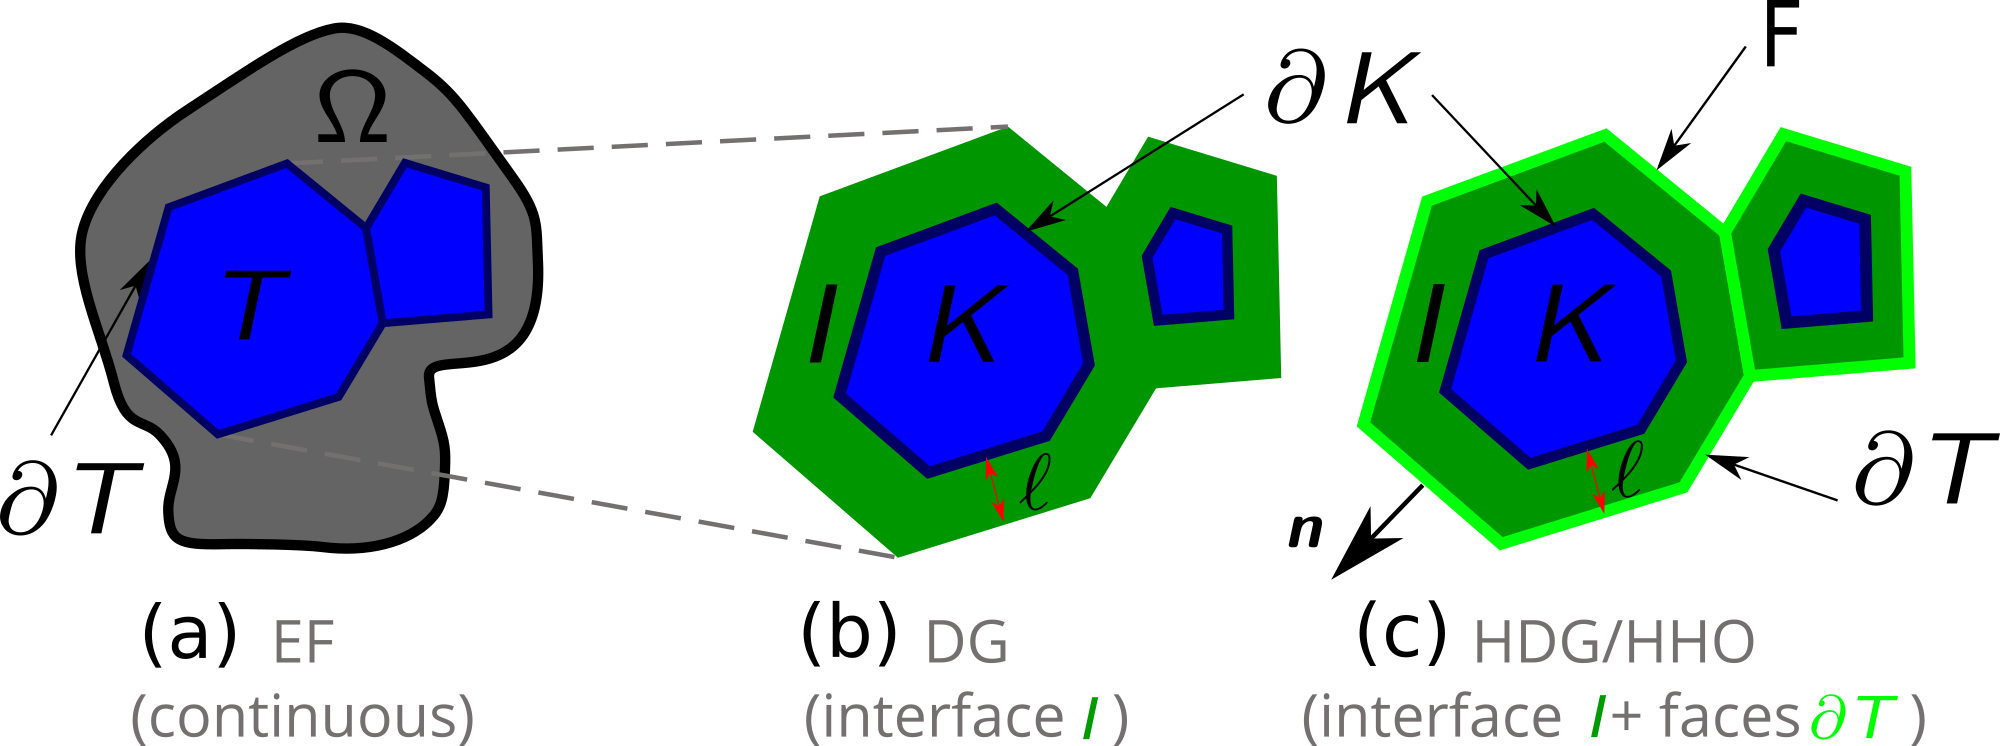
\includegraphics[width=14.cm]{../chapter_002_hho_mechanics/figures/ef_dg_hdg.png}
    \caption{schematic representation of a cell and its surrounding depending on the continuity requirement of the displacement field}
    \label{fig_02}
\end{figure}

% ---------------------------------------------------------
% PARAGRAPH
% ---------------------------------------------------------
\paragraph{Element loading}

The core $\Bulk$ is subjected to the volumetric loading $\loadLag{}$, and to the traction force applied by the interface $\Crown{}$ onto $\dBulk{}$. By continuity, $\Bulk{}$ applies the opposite traction force on $\Crown{}$ through $\dBulk{}$. The interface $\Crown{}$ is also subjected to the exterior traction force $\neumannCellLoad{}$ acting on $\neumannCell{}$, that accounts for the action of the rest of the solid $\bodyLag{}$ onto the boundary $\dCell$.

% ---------------------------------------------------------
% PARAGRAPH
% ---------------------------------------------------------
\paragraph{Discplacement, displacement gradient and stress fields}

Let note $\tensori{u}{}_{\Bulk}$ the displacement field, $\tensorii{G}{}_{\Bulk}$ the displacement gradient field and $\tensorii{P}{}_{\Bulk}$ the stress field in $\Bulk{}$. Similarly, let $\tensori{u}{}_{\Crown{}}$ the displacement field, $\tensorii{G}{}_{\Crown}$ the displacement gradient field and $\tensorii{P}{}_{\Crown}$ the stress field in $\Crown{}$.
The displacement of the boundary $\dCell{}$ is denoted $\tensori{u}{}_{\dCell{}}$.
By continuity of the displacement field between $\Bulk{}$ and $\dCell$,  the displacement $\tensori{u}{}_{\Crown{}}$ verifies
%
% 
% 
\begin{subequations}
    \label{eq_conformity}
        \begin{alignat}{2}
        \tensori{u}{}_{\Crown} \vert_{\dBulk} & = \tensori{u}{}_{\Bulk} \vert_{\dBulk}
        \label{eq_conformity:eq1},
        \\
        \tensori{u}{}_{\Crown} \vert_{\dCell} & = \tensori{u}{}_{\dCell}
        \label{eq_conformity:eq2}.
    \end{alignat}
\end{subequations}
%
%
%
Moreover, since the interface is of negligible volume compared to that of the core,
let assume that $\Field{\DisplacementField}{\Crown}{}$ linearly bridges
$\Field{\DisplacementField}{\dCell}{}$ to 
$\Field{\DisplacementField}{\Bulk}{}$.
As a result, the gradient of the displacement $\nabla \Field{\DisplacementField}{\Crown}{}$ is homogeneous in $\Crown{}$ along $\tensori{n}$.
Finally, the normal stress is assumed to be continuous across the inner boundary $\dBulk$, such that
%
% 
% 
\begin{equation}
    \label{eq_continuity_traction_force}
    \begin{aligned}
        (\tensorii{P}{}_{\Crown} - \tensorii{P}{}_{\Bulk} \vert_{\dBulk{}}) \cdot \tensori{n}{} = 0
        &&
        \text{on}
        &&
        \dBulk{}.
        % &&
        % \text{in}
        % &&
        % \Crown{}
    \end{aligned}
\end{equation}

% ---------------------------------------------------------
% PARAGRAPH
% ---------------------------------------------------------
\paragraph{Element behaviour}

The core of the element $\Bulk{}$ is made out of the same material that composes $\bodyLag$ and behaves
according to the free energy potential $\mecPotential{}_{\bodyLag{}}$.
The interface $\Crown{}$ is made out of a pseudo linear elastic material of
Young modulus $\beta (\ell / h_{\cell})$ with a zero Poisson ratio and its behavior is defined
by the free energy potential $\mecPotential{}_{\Crown{}}$ such that
%
%
%
\begin{equation}
    \label{eq_0009}
        \mecPotential{}_{\Crown} = \frac{1}{2} \beta \frac{\ell}{h_{\cell}} \nabla \tensori{u}{}_{\Crown} : \nabla \tensori{u}{}_{\Crown},
\end{equation}
%
%
%
where the dimensionless ratio $\ell / h_{\cell}$ balances the internal energy in the pseudo-elastic interface with that in the core part.

% ---------------------------------------------------------
% PARAGRAPH
% ---------------------------------------------------------
\paragraph{Hu-Washizu Lagrangian of the element}

By combining both the Lagragian of the core $\Bulk{}$ and that of the interface $\Crown{}$, one obtains the total Lagragian $L_{\cell}^{HW}$ over the element such that
%
%
%
\begin{equation}
    \label{eq_hu_washizu_split}
    L_{\cell}^{HW}
    % (\tensori{u}{}_{\cell}, \tensorii{G}{}_{\cell}, \tensorii{P}{}_{\cell})
    =
    \int_{\Bulk} \mecPotential_{\bodyLag{}} + \int_{\Bulk} (\nabla \tensori{u}{}_{\Bulk} - \tensorii{G}{}_{\Bulk}) : \tensorii{P}{}_{\Bulk}
    +
    \int_{\Crown} \mecPotential_{\Crown{}} + \int_{\Crown} (\nabla \tensori{u}{}_{\Crown} - \tensorii{G}{}_{\Crown}) : \tensorii{P}{}_{\Crown}
    -
    \int_{\Bulk} \loadLag \cdot \tensori{u}{}_{\Bulk}
    % -
    % \int_{\Crown} \loadLag \cdot \tensori{u}{}_{\Crown}
    -
    \int_{\neumannCell} \neumannCellLoad \cdot \tensori{u}{}_{\dCell},
\end{equation}

% % ---------------------------------------------------------
% % -- SUBSECTION
% % ---------------------------------------------------------
% \subsection{Hypotheses}
% \label{sec_assumtions}

% % Since the interface is of negligible volume compared to that of the core, the following assumptions are made on the displacement and the stress fields in the interface:

% % ---------------------------------------------------------
% % PARAGRAPH
% % ---------------------------------------------------------
% \paragraph{Displacement in the interface}

% Since the interface is of negligible volume compared to that of the core,
% let assume that $\Field{\DisplacementField}{\Crown}{}$ the displacement of the interface $\Crown{}$ linearly bridges
% $\Field{\DisplacementField}{\dCell}{}$ the displacement of the boundary $\dCell{}$ to 
% $\Field{\DisplacementField}{\Bulk}{}$ that  of the bulk $\Bulk{}$.
% As a result, the gradient of the displacement $\nabla \Field{\DisplacementField}{\Crown}{}$ is homogeneous in $\Crown{}$ along $\tensori{n}$.

% % Since the interface is of negligible volume compared to that of the core, the displacement in the interface $\Crown$ is assumed to be linear with respect to $\tensori{n}$, such that
% % its gradient is homogeneous in $\Crown{}$ along $\tensori{n}$
% % %
% % % 
% % % 
% % \begin{equation}
% %     \label{eq_crown_displacement}
% %     \nabla
% %     \tensori{u}{}_{\Crown}
% %     =
% %     \frac{\tensori{u}{}_{\dCell}
% %     -
% %     \tensori{u}{}_{\Bulk} \vert_{\dBulk} }{\ell} \otimes \tensori{n}.
% % \end{equation}
% % % 
% % % 
% % %
% % That is, the displacement of the interface $\Crown{}$ linearly bridges that of the boundary $\dCell{}$ to that of the bulk $\Bulk{}$.

% % ---------------------------------------------------------
% % PARAGRAPH
% % ---------------------------------------------------------
% \paragraph{Stress in the interface}

% % Likewise the stress field in the interface $\Field{\PKIStressField}{\Crown}{}$ is assumed to be constant along the direction $\tensori{n}{}$ in $\Crown{}$.
% The normal stress is assumed to be continuous across the inner boundary $\dBulk$, such that
% %
% % 
% % 
% \begin{equation}
%     \label{eq_continuity_traction_force}
%     \begin{aligned}
%         (\tensorii{P}{}_{\Crown} - \tensorii{P}{}_{\Bulk} \vert_{\dBulk{}}) \cdot \tensori{n}{} = 0
%         &&
%         \text{on}
%         &&
%         \dBulk{}.
%         % &&
%         % \text{in}
%         % &&
%         % \Crown{}
%     \end{aligned}
% \end{equation}

% Likewise, let assume that $\tensorii{P}{}_{\Crown}$ is constant along the direction $\tensori{n}{}$ in $\Crown{}$. By continuity of the traction force across $\dBulk$, the following equality holds true
% %
% % 
% % 
% \begin{equation}
%     \label{eq_continuity_traction_force}
%     \begin{aligned}
%         (\tensorii{P}{}_{\Crown} - \tensorii{P}{}_{\Bulk} \vert_{\dBulk{}}) \cdot \tensori{n}{} = 0
%         &&
%         \text{on}
%         &&
%         \dBulk{}.
%         % &&
%         % \text{in}
%         % &&
%         % \Crown{}
%     \end{aligned}
% \end{equation}

% ---------------------------------------------------------
% -- SUBSECTION
% ---------------------------------------------------------
\subsection{Towards Hybrid discontinuous methods from the Hu-Washizu Lagrangian}

% Using the hypotheses stated in Section \ref{sec_assumtions} on the displacement and the stress field in $\Crown{}$,
% \eqref{eq_hu_washizu_split} can be expressed as a term depending on the thickness of the interface $\ell$ and on the core and boundary unknowns only.
% In particular, making the thickness of the interface $\ell \rightarrow 0$, such that $\Crown{}$ vanishes and the core part $\Bulk{}$ identifies to $\cell$,
% a simplified expression of \eqref{eq_hu_washizu_split} is obtained.
% The reader can refer to \ref{sec_appendix_Hu_Washizu} for more details on technical details.

% ---------------------------------------------------------
% PARAGRAPH
% ---------------------------------------------------------
\paragraph{Simplified Hu–Washizu Lagrangian for a vanishing interface}

% In particular, making the thickness of the interface $\ell \rightarrow 0$, such that $\Crown{}$ vanishes and the core part $\Bulk{}$ identifies to $\cell$,
% The following simplified Hu–Washizu Lagrangian is obtained (See \ref{sec_appendix_Hu_Washizu})
% Using hypotheses expressed in Section \ref{sec_assumtions} and making $\ell \rightarrow 0$, the following simplified Hu–Washizu Lagrangian arises from \eqref{eq_hu_washizu_split}
Using the hypotheses stated in Section \ref{sec_assumtions} on the displacement and the stress field in $\Crown{}$, the Lagrangian
\eqref{eq_hu_washizu_split} can be expressed as a term depending on the thickness of the interface $\ell$ and on the core and boundary unknowns only.
In particular, making the thickness of the interface $\ell \rightarrow 0$, such that $\Crown{}$ vanishes and the core part $\Bulk{}$ identifies to $\cell$,
a simplified expression of \eqref{eq_hu_washizu_split} is obtained such that
% 
% 
%
\begin{equation}
    \label{eq_0015}
    \begin{aligned}
        L_{\cell}^{HW}
        = &
        \int_{\cell{}} \mecPotential{}_{\bodyLag{}} + \int_{\cell{}} (\nabla \tensori{u}{}_{\cell{}} - \tensorii{G}{}_{\cell{}}) : \tensorii{P}{}_{\cell}
        % \\
        % &
        + \int_{\dCell{}} (\tensori{u}{}_{\dCell} - \tensori{u}{}_{\cell} \vert_{\dCell}) \cdot \tensorii{P}{}_{\cell} \vert_{\dCell{}} \cdot \tensori{n}{}
        % \\
        % &
        + \int_{\dCell} \frac{\beta}{2 h_{\cell}} \lVert \tensori{u}{}_{\dCell{}} - \tensori{u}{}_{\cell{}} \vert_{\dCell{}} \rVert^2
        \\
        &
        -
        \int_{\cell} \loadLag{} \cdot \tensori{u}{}_{\cell{}}
        -
        \int_{\neumannCell{}} \neumannCellLoad{} \cdot \tensori{u}{}_{\dCell{}},
    \end{aligned}
\end{equation}
%
%
%
where \eqref{eq_0015} fully defines the equilibrium of an element in the context of hybrid discontinuous methods. The reader can refer to \ref{sec_appendix_Hu_Washizu} for technical details.

% ---------------------------------------------------------
% PARAGRAPH
% ---------------------------------------------------------
\paragraph{HDG methods and hybridization of the primal unknown}

Since the interface $\Crown{}$ has vanished, both $\tensori{u}{}_{\cell} \vert_{\dCell{}}$ the trace of the displacement of the core part $\cell$ onto $\dCell{}$ and $\tensori{u}{}_{\dCell{}}$ the displacement of the boundary coexist on $\dCell{}$. The displacement of the element $\cell$ is thus said to be \textit{hybrid}, and is denoted by the pair $(\tensori{u}{}_{\cell}, \tensori{u}{}_{\dCell})$.

% ---------------------------------------------------------
% PARAGRAPH
% ---------------------------------------------------------
\paragraph{The special case of DG methods}

Replacing $\tensori{u}{}_{\dCell}$ by $\tensori{u}{}_{\cell'} \vert_{\dCell}$ for any neighboring cell $\cell'$ amounts to describe the framework of Discontinuous Galerkin methods, where only the core unknown $\tensori{u}{}_{\cell}$ is considered, and the displacement jump on $\dCell$ depends on $\tensori{u}{}_{\cell'} \vert_{\dCell}$ the trace of the displacement of neighboring cells instead.

% ---------------------------------------------------------
% PARAGRAPH
% ---------------------------------------------------------
\paragraph{Conformal Galerkin formulation}

By strongly enforcing continuity of the displacement across $\dCell{}$ such that $\tensori{u}_{\cell} \vert_{\dCell} = \tensori{u}_{\dCell}$, one recovers the Principle of Virtual Work \eqref{eq_HW_0}, which defines the framework of conformal methods.

% ---------------------------------------------------------
% PARAGRAPH
% ---------------------------------------------------------
\paragraph{Lagrangian variations}

By differentiation of the total Lagrangian \eqref{eq_0015} with respect to each variable of the problem, the following weak equations arise
%
%
%
\begin{subequations}
    \label{eq_0017}
        \begin{alignat}{3}
            \langle \frac{\partial L_{\cell}^{HW}}{\partial \tensori{u}{}_{\cell}} , \delta \tensori{u}{}_{\cell} \rangle
            = & \int_{\cell} \tensorii{P}{}_{\cell} : \nabla \delta \tensori{u}{}_{\cell}
            -
            \int_{\cell} \tensori{f}{}_V \cdot \delta \tensori{u}{}_{\cell}
            -
            \int_{\dCell{}} \tensori{\theta}{}_{\cell} \cdot \delta \tensori{u}{}_{\cell} \vert_{\dCell}
            &&
            \qquad
            &&
            \forall \delta \tensori{u}{}_{\cell},
            % \in \virtualDisplacementSpaceCell
        \label{eq_0017:eq0}
        \\
            \langle \frac{\partial L_{\cell}^{HW}}{\partial \tensori{u}{}_{\dCell}} , \delta \tensori{u}{}_{\dCell} \rangle
            = &
            \int_{\neumannCell} (\tensori{\theta}{}_{\cell} - \tensori{t}{}_{\neumannCell}) \cdot \delta \tensori{u}{}_{\dCell}
            &&
            \qquad
            &&
            \forall \delta \tensori{u}{}_{\dCell},
            % \in \virtualDisplacementSpaceDCell
        \label{eq_0017:eq1}
        \\
            \langle \frac{\partial L_{\cell}^{HW}}{\partial \tensorii{P}{}_{\cell}} , \delta \tensorii{P}{}_{\cell} \rangle
            = & \int_{\cell} (\nabla \tensori{u}{}_{\cell} - \tensorii{G}{}_{\cell} ) : \delta \tensorii{P}{}_{\cell}
            +
            \int_{\dCell} (\tensori{u}{}_{\dCell} - \tensori{u}{}_{\cell} \vert_{\dCell}) \cdot \delta \tensorii{P}{}_{\cell} \vert_{\dCell} \cdot \tensori{n}{}
            &&
            \qquad
            &&
            \forall \delta \tensorii{P}{}_{\cell},
            % \in \stressSpaceCell
        \label{eq_0017:eq3}
        \\
            \langle \frac{\partial L_{\cell}^{HW}}{\partial \tensorii{G}{}_{\cell}} , \delta \tensorii{G}{}_{\cell} \rangle
            = &
            \int_{\cell} (\frac{\partial \mecPotential_{\bodyLag}}{\partial \tensorii{G}{}_{\cell}} - \tensorii{P}{}_{\cell}) : \delta \tensorii{G}{}_{\cell}
            &&
            \qquad
            &&
            \forall \delta \tensorii{G}{}_{\cell},
            % \in \gradSpaceCell
        \label{eq_0017:eq2}
    \end{alignat}
\end{subequations}
% 
% 
%
where the \textit{reconstructed traction force}
$\tensori{\theta}{}_{\cell} = \tensorii{P}{}_{\cell} \vert_{\dCell} \cdot \tensori{n}{} + (\beta / h_{\cell}) \tensori{J}(\tensori{u}{}_{\cell}, \tensori{u}{}_{\dCell})$ is introduced, with
$\tensori{J}(\tensori{u}{}_{\cell}, \tensori{u}{}_{\dCell}) = \tensori{u}{}_{\dCell} - \tensori{u}{}_{\cell} \vert_{\dCell}$ the jump function on the boundary $\dCell$.
Following discretization, multiple jump function choices are available.
The reader can refer to \ref{sec_stabilization} for more details regarding implementation aspects.
In particular, \eqref{eq_0017:eq0} is the expression of the Principle of Virtual Work in $\cell$,
where the \textit{reconstructed traction force} $\tensori{\theta}{}_{\cell}$ replaces the usual expression
$\tensorii{P}{}_{\cell} \cdot \tensori{n}{}$ in the external contribution. \eqref{eq_0017:eq1} denotes a supplementary equation to the usual
continuous problem as described in \eqref{eq_hu_washizu_derivative_0}, to account for the continuity of the flux $\tensori{\theta}{}_{\cell}$
across the cell boundary.
\eqref{eq_0017:eq2} accounts for the constitutive equation in a weak sense, and \eqref{eq_0017:eq3} defines the equation of an enhanced gradient field,
that does not reduce to the projection of $\nabla \tensori{u}{}_{\cell}$ as in \eqref{eq_hu_washizu_derivative_0:eq3}, since it is enriched by a
boundary component that depends on the displacement jump.
This feature is at the origin of the robustness of non-conformal methods to volumetric locking (see \ref{sec_appendix_gradient} for more details on this note).

\paragraph{Links with previous works}

The weak equations \eqref{eq_0017} are those defining the HDG problem introduced as in \cite{kabaria_hybridizable_2015}.
Though the equations are the same, they have been obtained here by the minimization of a total Lagrangian that also introduces
the definition of the so-called \textit{DG-derivative}
(which identifies with Equation \eqref{eq_0017:eq3}, and which is denoted here as the \textit{reconstructed gradient} in the following).
Moreover, in this paper, the discontinuity of the displacement is obtained by considering the limit case of a vanishing volumetric interface,
whereas if it postulated \textit{a priori} in \cite{kabaria_hybridizable_2015}.

% ---------------------------------------------------------
% -- SUBSECTION
% ---------------------------------------------------------
\subsection{Problem in primal form}
\label{sec_hdg_element_equilibrium}

% ---------------------------------------------------------
% PARAGRAPH
% ---------------------------------------------------------
\paragraph{Reconstructed gradient}

Since minimization of \eqref{eq_0017:eq3} defines a linear problem with any displacement pair $(\tensori{v}{}_{\cell}, \tensori{v}{}_{\dCell})$, one can eliminate \eqref{eq_0017:eq3} from the system \eqref{eq_0017}. The resulting equation defines the so-called \textit{reconstructed gradient} $\tensorii{G}{}_{\cell}(\tensori{v}{}_{\cell}, \tensori{v}{}_{\dCell})$ associated with any displacement pair $(\tensori{v}{}_{\cell}, \tensori{v}{}_{\dCell})$, that satisfies
%
%
%
\begin{equation}
    \label{eq_grad}
    \begin{aligned}
        \int_{\cell} \tensorii{G}{}_{\cell} : \tensorii{\tau}{}_{\cell}
        =
        \int_{\cell}  \nabla \tensori{v}{}_{\cell} : \tensorii{\tau}{}_{\cell}
        +
        \int_{\dCell} (\tensori{v}{}_{\dCell} - \tensori{v}{}_{\cell} \vert_{\dCell}) \cdot \tensorii{\tau}{}_{\cell} \vert_{\dCell} \cdot \tensori{n}{}
        &&
        \forall \tensorii{\tau}{}_{\cell},
        % \in \stressSpaceCell
    \end{aligned}
\end{equation}
%
%
%
where $\tensorii{\tau}{}_{\cell}$ denotes an arbitrary kinematically admissible stress field.
In particular, the \textit{reconstructed gradient} defined by Equation \eqref{eq_grad} identifies to that introduced in
\cite{di_pietro_hybrid_2015,abbas_hybrid_2018, abbas_hybrid_2019}.

% -> expliquer que quand saut tend vers 0, on retrouve le projection normale
%  ordre du gradient -> dire que même ordre que approximation primale, renvoie aux annexes

% ---------------------------------------------------------
% PARAGRAPH
% ---------------------------------------------------------
\paragraph{Stress tensor}

Likewise, \eqref{eq_0017:eq2} is eliminated from \eqref{eq_0017} since it is linear with $\tensorii{G}{}_{\cell}$. Assuming in addition that the space of kinematically admissible stress fields is included in that of kinematically admissible displacement gradient fields, \eqref{eq_0017:eq2} holds in a strong sense such that
%
%
%
\begin{equation}
    \label{eq_stress}
    \begin{aligned}
        \tensorii{P}{}_{\cell} = \frac{\partial \mecPotential_{\bodyLag}}{\partial \tensorii{G}{}_{\cell}}.
    \end{aligned}
\end{equation}

% ---------------------------------------------------------
% PARAGRAPH
% ---------------------------------------------------------
\paragraph{Lagrangian variations in primal form}

Using \eqref{eq_stress} and \eqref{eq_grad}, problem \eqref{eq_0017} depends on the displacement unknowns only.
% and the only remaining variations of the total Lagrangian \eqref{eq_0015} are those with respect to both displacement variables.
A new total Lagrangian $L_{\cell}^{HDG}$ arises from the simplified problem such that
%
%
%
\begin{equation}
    \label{eq_total_lagragian_bis}
    \begin{aligned}
        L_{\cell}^{HDG}
        = &
        \int_{\cell{}} \mecPotential_{\bodyLag}
        +
        \int_{\dCell} \frac{\beta}{2 h_{\cell}} \lVert \tensori{J}(\tensori{u}{}_{\cell{}}, \tensori{u}{}_{\dCell{}}) \rVert^2
        -
        \int_{\cell} \loadLag{} \cdot \tensori{u}{}_{\cell{}}
        -
        \int_{\neumannCell{}} \neumannCellLoad{} \cdot \tensori{u}{}_{\dCell{}},
    \end{aligned}
\end{equation}
%
%
%
with respective cell and boundary displacement variations:
\begin{subequations}
    \label{eq_final_problem}
        \begin{alignat}{3}
            \langle \frac{\partial L_{\cell}^{HDG}}{\partial \tensori{u}{}_{\cell}} , \delta \tensori{u}{}_{\cell} \rangle
            = & \int_{\cell} \tensorii{P}{}_{\cell} : \nabla \delta \tensori{u}{}_{\cell}
            -
            \int_{\cell} \tensori{f}{}_V \cdot \delta \tensori{u}{}_{\cell}
            -
            \int_{\dCell{}} \tensori{\theta}{}_{\cell} \cdot \delta \tensori{u}{}_{\cell} \vert_{\dCell}
            &&
            \qquad
            &&
            \forall \delta \tensori{u}{}_{\cell},
            % \in \virtualDisplacementSpaceCell
        \label{eq_final_problem:eq0}
        \\
            \langle \frac{\partial L_{\cell}^{HDG}}{\partial \tensori{u}{}_{\dCell}} , \delta \tensori{u}{}_{\dCell} \rangle
            = &
            \int_{\neumannCell} (\tensori{\theta}{}_{\cell} - \tensori{t}{}_{\neumannCell}) \cdot \delta \tensori{u}{}_{\dCell}
            &&
            \qquad
            &&
            \forall \delta \tensori{u}{}_{\dCell},
        \label{eq_final_problem:eq1}
    \end{alignat}
\end{subequations}
%
%
%
where $\tensorii{P}{}_{\cell}$ is defined by \eqref{eq_stress} and
depends on $\tensorii{G}{}_{\cell}$ which solves \eqref{eq_grad}.

\subsection{Restriction to the Small strain hypothesis}

The proposed large deformation formulation also allows for a natural transition to the small deformation framework. In this context, the gradient of the transformation $\tensorii{F}{}_{\cell}$ is assumed to be small compared to the identity $\tensorii{I}$, and the infinitesimal deformation field $\tensorii{\varepsilon}_{\cell}$ is sought in place of $\tensorii{F}{}_{\cell}$ such that
% \eqref{eq_grad_def} writes
%
%
%
\begin{equation}
    \tensorii{\varepsilon}{}_{\cell} - \nabla^s \tensori{u}{}_{\cell} = 0,
\end{equation}
%
%
%
where the symmetric displacement gradient $\nabla^s \tensori{u}{}_{\cell}$ replaces 
the usual displacement gradient in \eqref{eq_grad_def}.
The stress tensor $\tensorii{P}{}_{\cell}$ is then identified with the Cauchy stress $\tensorii{\sigma}{}_{\cell}$, such that the Lagrangian \eqref{eq_0015} becomes
%
%
%
\begin{equation}
    \label{eq_small_defs}
    \begin{aligned}
        L_{\cell}^{HW}
        = &
        \int_{\cell{}} \mecPotential{}_{\bodyLag{}} + (\nabla^s \tensori{u}{}_{\cell{}} - \tensorii{\varepsilon}{}_{\cell{}}) : \tensorii{\sigma}{}_{\cell}
        % \\
        % &
        + \int_{\dCell{}} (\tensori{u}{}_{\dCell} - \tensori{u}{}_{\cell} \vert_{\dCell}) \cdot \tensorii{\sigma}{}_{\cell} \vert_{\dCell{}} \cdot \tensori{n}{}
        % \\
        % &
        + \int_{\dCell} \frac{\beta}{2 h_{\cell}} \lVert \tensori{u}{}_{\dCell{}} - \tensori{u}{}_{\cell{}} \vert_{\dCell{}} \rVert^2
        \\
        &
        -
        \int_{\cell} \loadLag{} \cdot \tensori{u}{}_{\cell{}}
        -
        \int_{\neumannCell{}} \neumannCellLoad{} \cdot \tensori{u}{}_{\dCell{}},
    \end{aligned}
\end{equation}
%
%
%
where for any pair $(\tensori{v}{}_{\cell}, \tensori{v}{}_{\dCell})$ the \textit{reconstructed strain} $\tensorii{\varepsilon}{}_{\cell}(\tensori{v}{}_{\cell}, \tensori{v}{}_{\dCell})$ is evaluated against any kinematically admissible symmetric stress field $\tensorii{\tau}{}_{\cell}$ such that
%
%
%
\begin{equation}
    \label{eq_grad_ss}
    \begin{aligned}
        \int_{\cell} \tensorii{\varepsilon}{}_{\cell} : \tensorii{\tau}{}_{\cell}
        =
        \int_{\cell}  \nabla^s \tensori{v}{}_{\cell} : \tensorii{\tau}{}_{\cell}
        +
        \int_{\dCell} (\tensori{v}{}_{\dCell} - \tensori{v}{}_{\cell} \vert_{\dCell}) \cdot \tensorii{\tau}{}_{\cell} \vert_{\dCell} \cdot \tensori{n}{}
        &&
        \forall \tensorii{\tau}{}_{\cell},
        % \in \stressSpaceCell
    \end{aligned}
\end{equation}
%
%
%
and the Cauchy stress is the derivative of the potential $\mecPotential_{\bodyLag{}}$ with respect to $\tensorii{\varepsilon}{}_{\cell}$
%
%
%
\begin{equation}
    \label{eq_stress_ss}
    \begin{aligned}
        \tensorii{\sigma}{}_{\cell} = \frac{\partial \mecPotential_{\bodyLag}}{\partial \tensorii{\varepsilon}{}_{\cell}}.
    \end{aligned}
\end{equation}

% \subsection{Extension to the axi-symmetric framework}

% In the following section, we devise a Hybrid High order method for an axi-symmetric framework. Owing to geometrical assumptions on the displacement and its gradient, the definition of the reconstructed gradient \eqref{eq_grad} and of that of the higher order displacement \eqref{eq_potential} needs be modified accordingly. Details about the definitions of these ingredients can be found in \ref{sec_appendix_axi}.

% \paragraph{Axi-symmetric framework}

% The cartesian space is expressed in cylindrical coordinates and a point $\tensori{X} \in \bodyLag$ has coordinates $\tensori{X} = (r, z, \theta)$ where $r$ denotes the radial component, $z$ the ordinate one, and $\theta$ is the angular component describing a revolution around the axis $r = 0$. By cylindrical symmetry, the angular displacement $\tensoro{u}{}_{\theta}$ is supposed to be zero, and both components $u_r$ and $u_z$ do not depend on the angular coordinate $\theta$.

% % \paragraph{Cell displacement gradient}

% % % Adopting notations introduced in Section \ref{sec_composite_demo}, let $\cell$ an open subset of $\bodyLag \subset \mathbb{R}^2$ in the $(r,z)$ plane with cell displacement $\tensori{u}{}_{\cell} \in \displacementSpaceCell$ and boundary displacement $\tensori{u}{}_{\dCell} \in \displacementSpaceDCell$.
% % The partial derivatives of $\tensori{u}{}_{\cell}$ with respect to the cylindrical coordinates are given by
% % %
% % %
% % %
% % \begin{equation}
% %     \begin{aligned}
% %         \forall i, j \in \{ r,z \}, \tensoro{u}{}_{\cell i,j} = \frac{\partial u_{\cell i}}{\partial j} && \text{and} && \tensoro{u}{}_{\cell \theta, \theta} = \frac{u_{\cell r}}{r}
% %     \end{aligned}
% % \end{equation}

% \paragraph{Axis faces treatment}

% Since in cylindrical coordinates, all integrals depend on the radial component $r$, boundary integrals vanish at $r = 0$ on the symmetry axis.
% Therefore, the reconstructed gradient (and the stabilization) do not depend on a closed surface wrapping a cell $\cell$ located on the symmetry axis.
% However, this feature is necessary to prove the robustness of the HHO method to volumetric locking (see \ref{sec_appendix_gradient}).
% Therefore, in order to restore full mobility of a face located on the symmetry axis, we consider infinitely thin cylindrical faces wrapping it, that are subjected to Dirichlet boundary conditions along the radial direction.


%%
%
%
% ---------------------------------------------------------
% ---- SECTION
% ---------------------------------------------------------
\section{Discretization}
\label{sec-discretization}

This section specifies the nature of the so-called hybrid mesh,
and introduces the discretization for both cell and faces displacement fields.
The classical \textit{static condensation} cell unknowns elimination strategy is presented, and a novel elimination scheme
based on the previous Lagrangian formulation of hybrid discontinuous methods is then devised.

% ---------------------------------------------------------
% -- SUBSECTION
% ---------------------------------------------------------
\subsection{Mesh and skeleton}

% ---------------------------------------------------------
% PARAGRAPH
% ---------------------------------------------------------
\paragraph{Faces and skeleton of the mesh}

The boundary $\dCell{}$ of each element is decomposed in faces, such
that a face $F$ is a subset of $\bodyLag$, and either there are two
cells $\cell_F$ and $\cell_F'$ such that $F = \dCell_F \cap \dCell_F'$
($F$ is then an interior face), or there is a single cell $\cell_F$ such
that $F = \dCell_F \cap \partial \Omega$ ($F$ is then an exterior face).
Let $\dHybridMesh(\bodyLag) = \{ F_i \subset \bodyLag \ \vert \ 1 \leq i
\leq N_{F} \}$ the skeleton of the mesh, collecting all element faces
$F_i$ in the mesh, where $N_{F}$ denotes the number of faces. The set of
faces subjected to Neumann boundary conditions is denoted
$\dHybridMesh{}_{N}^e(\bodyLag)$, and $\dHybridMesh{}_{D}^e(\bodyLag)$
denotes that subjected to Dirichlet boundary conditions. Moreover, let
$\mathcal{F}^i(\bodyLag)$ the set of interior faces. For any cell
$\cell$, let $\mathcal{F}(\cell) = \{ F \in \dHybridMesh \ \vert \ F
\subset \dCell \}$ the set of faces composing the boundary of $\cell$,
and let $N_{\dCell}$ the number of faces in $\dCell$.

% ---------------------------------------------------------
% PARAGRAPH
% ---------------------------------------------------------
\paragraph{Mesh description}

Likewise, one defines the collection of all cells in the mesh
as $\HybridMesh(\bodyLag) = \{ \matI \subset \bodyLag \ \vert \ 1 \leq i
\leq N_{\cell} \}$, where $N_T$ denotes the total number of cells. The
composition of both $\mathcal{T}(\bodyLag)$ and
$\dHybridMesh{}(\bodyLag)$ forms the hybrid mesh
$\HybridMeshWhole({\bodyLag}) = \{ \mathcal{T}(\bodyLag),
\mathcal{F}(\bodyLag) \}$.

% ---------------------------------------------------------
% -- SUBSECTION
% ---------------------------------------------------------
\subsection{Discretization}

% ---------------------------------------------------------
% PARAGRAPH
% ---------------------------------------------------------
\paragraph{Discrete functional space}

Let $\discreteDisplacementSpaceCell$ denote an
approximation space of finite dimension for the displacement in the
cell, and $V^h(F)$ that on a face $F \in \mathcal{F}(\cell)$. The
approximation space on $\dCell$ is $V^h(\dCell) = \prod_{F \in
  \mathcal{F}(\cell)} V^h(F)$. Similarly, let $\discreteGradSpaceCell$
the approximation space of the reconstructed gradient and
$\discreteStressSpaceCell$ that chosen for the stress.

\paragraph{Approximation bases and elementary unknowns}

Let $\mathfrak{B}_T^h$ denote a polynomial basis of
$U^h(\cell)$, and $\mathfrak{B}_F^h$ a polynomial basis of $V^h(F)$, with respective dimensions $N_T^h$ and $N_F^h$.
The specific choice of monomial bases for
$\mathfrak{B}_T^h$ and $\mathfrak{B}_F^h$ is discussed in depth in
\ref{sec_appendix_implementation}, though other bases can be chosen.
Let $\tensori{u}{}_{T}^h \in U^h(T)$ the polynomial displacement field in $\cell$
and $\tensori{u}{}_{F}^h \in V^h(F)$ that of a face $F \subset \dCell$.
Using vector notations, $\tensori{u}{}_{T}^h$ (respectively $\tensori{u}{}_{F}^h$) can be represented by a vector of coefficients $\mathfrak{U}_T$ (respectively $\mathfrak{U}_F$)  in $\mathfrak{B}_T^h$ (respectively $\mathfrak{B}_F^h$) such that
% The displacement field $\tensori{u}{}_{T}^h \in U^h(T)$ (respectively $\tensori{u}{}_{F}^h \in V^h(F)$) is represented by a vector of
% coefficients $\mathfrak{U}_T$ of size $N_T^h$ in $\mathfrak{B}_T^h$ (respectively
% $\mathfrak{U}_F$ of size $N_F^h$ in $\mathfrak{B}_F^h$) such that
%
%
%
\begin{equation}
  \begin{aligned}
    \tensori{u}{}_{\cell}^h = \mathfrak{U}_T \cdot \mathfrak{B}_T^h
    &&
    \forall \cell \in \mathcal{T}(\bodyLag)
    &&
    \text{and}
    &&
    \tensori{u}{}_{F}^h = \mathfrak{U}_F \cdot \mathfrak{B}_F^h
    &&
    \forall F \in \mathcal{F}(\bodyLag)
  \end{aligned}
\end{equation}

\paragraph{Global Unknowns}

Let $(\tensori{u}{}_{\mathcal{T}}^h, \tensori{u}{}_{\mathcal{F}}^h)
\in U^h(\mathcal{T}) \times U^h(\mathcal{F})$ the global displacement
unknown of problem \eqref{eq_final_problem} in discrete form, where
$\tensori{u}{}_{\mathcal{T}}^h$ and $\tensori{u}{}_{\mathcal{F}}^h$ are
the piece-wise continuous displacements such that:
%
%
%
\begin{equation}
  \begin{aligned}
    \tensori{u}{}_{\mathcal{T}}^h
    \vert_{\cell} = \tensori{u}{}_{\cell}^h
    % = \mathfrak{U}_T \cdot \mathfrak{B}_T^h
    &&
    \forall \cell \in \mathcal{T}
    &&
    \text{and}
    &&
    \tensori{u}{}_{\mathcal{F}}^h \vert_{F}
    % = \tensori{u}{}_{F}^h = \mathfrak{U}_F \cdot \mathfrak{B}_F^h
    &&
    \forall F \in \mathcal{F}
  \end{aligned}
\end{equation}
% 
% 
% 
with $U^h(\mathcal{T}) = \prod_{T \in \mathcal{T}} U^h(T)$ and
$U^h(\mathcal{F}) = \prod_{F \in \mathcal{F}} U^h(F)$.
In the following, let
$\mathfrak{U}_{\mathcal{T}}$ the unknown coefficient vector associated
to $\tensori{u}{}^h_{\mathcal{T}}$ and $\mathfrak{U}_{\mathcal{F}}$ that to
$\tensori{u}{}^h_{\mathcal{F}}$.

\paragraph{Elementary boundary unknown}

Likewise, let $\tensori{u}{}_{\dCell}^h \in V^h(\dCell)$ such
that
%
%
%
\begin{equation}
  \begin{aligned}
    \tensori{u}{}_{\dCell}^h \vert_F = \tensori{u}{}_{F}^h
    &&
    \forall F \in \mathcal{F}(T)
  \end{aligned}
\end{equation}
% $\tensori{u}{}_{\dCell}^h \vert_F = \tensori{u}{}_{F}^h, \forall F
% \in \mathcal{F}(T)$.
%
%
%
% In the following, let
% $\mathfrak{U}_{\mathcal{T}}$ the unknown coefficient vector associated
% to $\tensori{u}{}^h_{\mathcal{T}}$, $\mathfrak{U}_{\mathcal{F}}$ that to
% $\tensori{u}{}^h_{\mathcal{F}}$, and $\mathfrak{U}_{\mathcal{\dCell}}$
% that to $\tensori{u}{}^h_{\dCell}$.
and let $\mathfrak{U}_{\mathcal{\dCell}}$
the unknown coefficient vector associated to $\tensori{u}{}^h_{\dCell}$.

% ---------------------------------------------------------
% -- SUBSECTION
% ---------------------------------------------------------
\subsection{Local and global discrete problems}

% ---------------------------------------------------------
% PARAGRAPH
% ---------------------------------------------------------
\subsubsection{Local residual}

As in a functional space of finite dimension, the restriction of a linear
form can be represented by a vector in the dual space, let
$\mathfrak{R}_{\cell}$ and $\mathfrak{R}_{\dCell}$ the residual vectors
associated with the the variations of the total
Lagrangian~\eqref{eq_total_lagragian_bis}:
\begin{subequations}
  \label{eq_final_problem_00}
  \begin{alignat}{3}
    \mathfrak{R}_{\cell}(\mathfrak{U}_{\cell},
    \mathfrak{U}_{\dCell}) \cdot \mathfrak{\hat{U}}_{T}
    % \int_{\mathcal{T}} R_{\mathcal{T}}(\tensori{u}{}_{\mathcal{T}}, \tensori{u}{}_{\mathcal{F}}) \cdot \tensori{\hat{u}}{}_{\mathcal{T}}
 = & \int_{\cell} \tensorii{P}{}_{\cell}^h : \nabla
    \tensori{\hat{u}}{}_{\cell}^h - \int_{\cell} \tensori{f}{}_V \cdot
    \tensori{\hat{u}}{}_{\cell} - \int_{\dCell{}}
    \tensori{\theta}{}_{\cell}^h \cdot \tensori{\hat{u}}{}_{\cell}^h
    \vert_{\dCell} && \ \ \ \ \ \ \ \ && \forall
    \hat{\mathfrak{U}}_{\cell} % \in \virtualDisplacementSpaceCell
    \label{eq_final_problem_00:eq0} \\
    \mathfrak{R}_{\dCell}(\mathfrak{U}_{\cell},
    \mathfrak{U}_{\dCell}) \cdot \mathfrak{\hat{U}}_{\dCell}
    % \int_{\mathcal{F}} R_{\mathcal{F}}(\tensori{u}{}_{\mathcal{T}}, \tensori{u}{}_{\mathcal{F}}) \cdot \tensori{\hat{u}}{}_{\mathcal{F}}
 = & \int_{\dCell} (\tensori{\theta}{}_{\cell}^h -
    \tensori{t}{}_{\neumannCell}) \cdot \tensori{\hat{u}}{}_{\dCell}^h
    && \ \ \ \ \ \ \ \ && \forall \hat{\mathfrak{U}}_{\dCell}
    % \in \virtualDisplacementSpaceDCell \label{eq_final_problem_00:eq1}
    \label{eq_final_problem_00:eq1} \\
  \end{alignat}
\end{subequations}
where the discrete stress tensor $\tensorii{P}{}_{\cell}^h$ and the
discrete reconstructed gradient
$\tensorii{G}{}_{\cell}^h(\tensori{v}{}_{\cell}^h,
\tensori{v}{}_{\dCell}^h)$ are defined by the discrete forms of
equations \eqref{eq_stress} and \eqref{eq_grad} respectively such that:
\begin{equation}
  \label{eq_stress_discrete}
  \begin{aligned}
    \tensorii{P}{}_{\cell}^h =
    \frac{\partial \mecPotential_{\bodyLag}}{\partial
      \tensorii{G}{}_{\cell}^h} && \text{and} && \int_{\cell}
    \tensorii{G}{}_{\cell}^h : \tensorii{\tau}{}_{\cell}^h =
    \int_{\cell} \nabla \tensori{v}{}_{\cell}^h :
    \tensorii{\tau}{}_{\cell}^h + \int_{\dCell}
    (\tensori{v}{}_{\dCell}^h - \tensori{v}{}_{\cell}^h \vert_{\dCell})
    \cdot \tensorii{\tau}{}_{\cell}^h \vert_{\dCell} \cdot \tensori{n}{}
    && \forall \tensorii{\tau}{}_{\cell}^h \in S^h(\cell)
  \end{aligned}
\end{equation}
%
%
%
and the discrete reconstructed traction writes
$\tensori{\theta}{}_{\cell}^h = \tensorii{P}{}_{\cell}^h \cdot \tensori{n} + (\beta / h_{\cell})
\tensori{J}^h(\tensori{v}{}_{\cell}^h, \tensori{v}{}_{\dCell}^h)$. In particular, the
expression of the discrete jump function $\tensori{J}^h(\tensori{v}{}_{\cell}^h, \tensori{v}{}_{\dCell}^h)$
is the key ingredient that defines the HHO method (see Section \ref{sec_appendix_implementation} for more details on this note).
The solution of the discrete problem
% $(\mathfrak{U}_{\cell}, \mathfrak{U}_{\dCell})$
is defined by the fact that the
residuals $\mathfrak{R}_{\cell}$ and $\mathfrak{R}_{\dCell}$ must be
zero
\begin{equation}
  \label{eq_final_problem_000}
  \begin{aligned}
    \mathfrak{R}_{\cell}(\mathfrak{U}_{\cell}, \mathfrak{U}_{\dCell})
    = 0 && \text{and} &&
    \mathfrak{R}_{\dCell}(\mathfrak{U}_{\cell}, \mathfrak{U}_{\dCell})
     = 0
  \end{aligned}
\end{equation}
%
%
%
In practice, the computation of $\mathfrak{R}_{\cell}$ and
$\mathfrak{R}_{\dCell}$ is discussed in depth in \ref{sec_appendix_implementation}.

% ---------------------------------------------------------
% PARAGRAPH
% ---------------------------------------------------------
\subsubsection{Global residuals and face assembly}

\paragraph{Global problem}

At the global scale, the solution
$(\mathfrak{U}_{\mathcal{T}}, \mathfrak{U}_{\mathcal{F}})$ of the
discrete problem satisfies:
\begin{equation}
  \label{eq_final_global_problem_0}
  \begin{aligned}
    \forall \cell \in \mathcal{T}(\bodyLag), \forall
    \hat{\mathfrak{U}}_{\cell},
    \mathfrak{R}_{\cell}(\mathfrak{U}_{\cell}, \mathfrak{U}_{\dCell})
    \cdot \mathfrak{\hat{U}}_{T} & = 0 && \text{and} && \forall
    \hat{\mathfrak{U}}_{\mathcal{F}},
    \mathfrak{R}_{\mathcal{F}}(\mathfrak{U}_{\mathcal{T}},
    \mathfrak{U}_{\mathcal{F}}) \cdot \mathfrak{\hat{U}}_{\mathcal{F}} =
    0
  \end{aligned}
\end{equation}
where the vector
$\mathfrak{R}_{\mathcal{F}}(\mathfrak{U}_{\mathcal{T}},
\mathfrak{U}_{\mathcal{F}})$ is the skeleton residual such that
\begin{equation}
  \label{eq_final_problem_0}
  \begin{aligned}
    \mathfrak{R}_{\mathcal{F}}(\mathfrak{U}_{\mathcal{T}},
    \mathfrak{U}_{\mathcal{F}}) \cdot \mathfrak{\hat{U}}_{\mathcal{F}}
    % \int_{\mathcal{F}} R_{\mathcal{F}}(\tensori{u}{}_{\mathcal{T}}, \tensori{u}{}_{\mathcal{F}}) \cdot \tensori{\hat{u}}{}_{\mathcal{F}}
 = & \sum_{F \in \mathcal{F}^i(\bodyLag{})} \int_{F}
    (\tensori{\theta}{}_{\cell_F}^h + \tensori{\theta}{}_{\cell_F '}^h)
    \cdot \tensori{\hat{u}}{}_{F}^h + \sum_{F \in
      \mathcal{F}^e_N(\bodyLag{})} \int_{F}
    (\tensori{\theta}{}_{\cell_F}^h - \neumannLag) \cdot
    \tensori{\hat{u}}{}_{F}^h && \forall
    \hat{\mathfrak{U}}_{\mathcal{F}}
  \end{aligned}
\end{equation}
%
%
%
and which results in the assembly of faces unknowns only.

\paragraph{Assembly over the skeleton}

An interior face $F$ is linked to two adjacent cells $T$ and $T'$, and
each of these cells applies to the other a surface load $\pm
\tensori{t}{}_{T\cap T'}$ through $F$, which is identified with
$\tensori{t}{}_{\neumannCell}$ on $F$ in \eqref{eq_final_problem_00:eq1}.
By summation over each face of the structure, these equal contributions
cancel out, which yields the expression of the first argument in the
right-hand side of \eqref{eq_final_problem_0}.
%
%
%
Since exterior faces subjected to Neumann boundary conditions are
linked to a single cell only, the local surface forces $\tensori{t}{}_{\neumannCell}$ are equal to $\neumannLag$ on $\neumannBoundaryLag{}$,
which yields the expression of
the second argument in the right-hand side of
\eqref{eq_final_problem_00:eq1}.

% ---------------------------------------------------------
% -- SUBSECTION
% ---------------------------------------------------------
\subsection{Cell unknowns elimination}
\label{sec_cell_unknowns_elimination}

As the cell number of unknowns grows rapidly with the polynomial order
as compared to that in the face (See \ref{sec_shape_functions} for further details), cell
unknowns must be eliminated for the for the method to be numerically
attractive.

In this section, two elimination strategies are examinated. The first
one, presented as the \textit{Cell equilibrium} strategy, has, to our
knowledge, never been introduced in the literature, and arises from the
previous total Lagrangian formulation of HDG methods. The second one
consists in performing a static condensation operation
\cite{abbas_hybrid_2018, abbas_hybrid_2019,di_pietro_hybrid_2015}
following linearization of the problem.

% ---------------------------------------------------------
% PARAGRAPH
% ---------------------------------------------------------
\subsubsection{Cell equilibrium}
\label{sec_cell_equilibrium_scheme}

This first algorithm considers that the cell displacement unknown
$\mathfrak{U}_{T}$ are defined as implicit functions of the boundary
displacement unknown $\mathfrak{U}_{\dCell}$ as follows:
\begin{equation}
  \label{eq_cell_equilibrium_1}
  \begin{aligned}
    \mathfrak{R}_{T}(\mathfrak{U}_{T}(\mathfrak{U}_{\dCell}),
    \mathfrak{U}_{\dCell}) = 0
  \end{aligned}
\end{equation}
In practice, Nonlinear Equation~\eqref{eq_cell_equilibrium_1} can be
solved by an iterative method.
%
%
%
At the global scale, the face residual can thus be expressed as
function of the face displacement only, and satisfies:
\begin{equation}
  \label{eq_cell_equilibrium_face_residual}
  \mathfrak{R}_{\mathcal{F}}(\mathfrak{U}_{\mathcal{T}}\paren{\mathfrak{U}_{\mathcal{F}}},
 \mathfrak{U}_{\mathcal{F}})=0
\end{equation}
%
%
%
Likewise, equation~\eqref{eq_cell_equilibrium_face_residual} is also
generally solved using an iterative method, where the face displacement is
the only unknown. Two algorithm are now presented:

\begin{itemize}
  \item The standard Newton algoritmh.
  \item A fixed point algorithm combined with an acceleration scheme.
\end{itemize}

\paragraph{Resolution of Nonlinear Equation~\eqref{eq_cell_equilibrium_face_residual} using the Newton algorithm}

Let \(\iter{n}{\mathfrak{U}_{\mathcal{F}}}\) be the current estimate
of the solution. The correction
\(\iter{n}{\delta}\mathfrak{U}_{\mathcal{F}}\) of this estimate is given
by:
\[
\iter{n}{\delta}\mathfrak{U}_{\mathcal{F}}=
-\left( \frac{d\mathfrak{R}_{\mathcal{F}}}{d \mathfrak{U}_{\mathcal{F}}}
\right)^{-1} \,\cdot\,\iter{n}{\mathfrak{R}}_{\mathcal{F}}
\]
with
\(\iter{n}{\delta}\mathfrak{U}_{\mathcal{F}}=\iter{n+1}{\mathfrak{U}_{\mathcal{F}}}-\iter{n}{\mathfrak{U}_{\mathcal{F}}}\).
%
%
%
The jacobian matrix \(\frac{d\mathfrak{R}_{\mathcal{F}}}{d
  \mathfrak{U}_{\mathcal{F}}}\) can be determined using the chain rule,
as follows:
\begin{equation}
  \label{eq_cell_equilibrium_0}
  \begin{aligned}
    \frac{d\mathfrak{R}_{\mathcal{F}}}{d
      \mathfrak{U}_{\mathcal{F}}}
    = \frac{\partial
      \mathfrak{R}_{\mathcal{F}}}{\partial \mathfrak{U}_{\mathcal{T}}}
    \frac{\partial \mathfrak{U}_{\mathcal{T}}}{\partial
      \mathfrak{U}_{\mathcal{F}}} \cdot \delta
    \mathfrak{U}_{\mathcal{F}} + \frac{\partial
      \mathfrak{R}_{\mathcal{F}}}{\partial \mathfrak{U}_{\mathcal{F}}}
    \cdot \delta \mathfrak{U}_{\mathcal{F}}
  \end{aligned}
\end{equation}
Applying the implicit function theorem to
\eqref{eq_cell_equilibrium_1} yields:
\begin{equation}
  \label{eq_cell_equilibrium_2}
  \begin{aligned}
    \frac{\partial
      \mathfrak{U}_{\mathcal{T}}}{\partial \mathfrak{U}_{\mathcal{F}}} =
    - \frac{\partial \mathfrak{U}_{\mathcal{T}}}{\partial
      \mathfrak{R}_{\mathcal{T}}} \frac{\partial
      \mathfrak{R}_{\mathcal{T}}}{\partial \mathfrak{U}_{\mathcal{F}}}
  \end{aligned}
\end{equation}
Injecting \eqref{eq_cell_equilibrium_2} in
\eqref{eq_cell_equilibrium_0} yields the expression of the derivative of
the face resiudal with respect to the face displacement
\begin{equation}
  \label{eq_cell_equilibrium_3}
  \begin{aligned}
    \frac{d\mathfrak{R}_{\mathcal{F}}}{d
      \mathfrak{U}_{\mathcal{F}}} = \frac{\partial
      \mathfrak{R}_{\mathcal{T}}}{\partial \mathfrak{U}_{\mathcal{F}}}
    \cdot \delta \mathfrak{U}_{\mathcal{F}} - \frac{\partial
      \mathfrak{R}_{\mathcal{T}}}{\partial \mathfrak{U}_{\mathcal{T}}}
    \frac{\partial \mathfrak{U}_{\mathcal{T}}}{\partial
      \mathfrak{R}_{\mathcal{T}}} \frac{\partial
      \mathfrak{R}_{\mathcal{T}}}{\partial \mathfrak{U}_{\mathcal{F}}}
    \cdot \delta \mathfrak{U}_{\mathcal{F}}
  \end{aligned}
\end{equation}

\paragraph{Resolution of Nonlinear
  Equation~\eqref{eq_cell_equilibrium_face_residual} using a accelerated
  fixed point algorithm} Nonlinear
Equation~\eqref{eq_cell_equilibrium_face_residual} can be rewritten as
follows:
\[
\mathfrak{U}_{\mathcal{F}}=
\mathfrak{U}_{\mathcal{F}}-\hat{\mathbb{K}}^{-1}\,\cdot\,\mathfrak{R}_{\mathcal{F}}\paren{\mathfrak{U}_{\mathcal{T}}\paren{\mathfrak{U}_{\mathcal{F}}},
 \mathfrak{U}_{\mathcal{F}}}
\]
where \(\hat{\mathbb{K}}\) is a preconditionning matrix. This equation leads to the following fixed iteration scheme:
\[
\iter{n+1}{\mathfrak{U}_{\mathcal{F}}}=\iter{n}{\mathfrak{U}_{\mathcal{F}}}
- \hat{\mathbb{K}}^{-1}\,\cdot\,\mathfrak{R}_{\mathcal{F}}\paren{\mathfrak{U}_{\mathcal{T}}\paren{\iter{n}{\mathfrak{U}_{\mathcal{F}}}},
  \iter{n}{\mathfrak{U}_{\mathcal{F}}}}
\]
%
%
%
It is clear that the Newton algorithm is recovered if
\(\hat{\mathbb{K}}\) is egal to
\(\derivtot{\mathfrak{R}_{\mathcal{F}}}{\mathfrak{U}_{\mathcal{F}}}\).
The idea of this algorithm is however to use a constant preconditionning
matrix.

In the authors' experience, the initial elastic stiffness matrix is an
appropriate choice for \(\hat{\mathbb{K}}\) in most cases. This strategy
has been used by default in the {\tt Cast3M} finite element solver for
years. One advantage of this method is that if a direct solver is used
to compute \(\hat{\mathbb{K}}^{-1}\,\cdot\,\mathfrak{R}_{\mathcal{F}}\),
the matrix \(\hat{\mathbb{K}}^{-1}\) only have to be decomposed once.
%
%
%
As expected, this fixed point algorithm leads to a linear convergence
(compared to the quadratic convergence of the Newton algorithm).
However, combined with acceleration schemes, this algorithm can be
competive with the Newton algorithm in many cases. The reader can refer to
\cite{ramiere_iterative_2015} for a discussion on this subject.
Numerical examples using such acceleration schemes are
evaluated in Section \ref{sec_numerical_examples}.
%
%
%
It is worth noticing that if efficient preconditionning operators
where available, this accelerated fixed-point scheme could be the basis
of a truly matrix-free algorithm. Using an incomplete decomposition of
the elastic stiffness matrix may be a first step in this direction.
Exploring this line of research is left for future works.

\subsubsection{Static condensation}
\label{sec_static_condesnation_scheme}

In this section, $\mathfrak{U}_{\mathcal{T}}$ and
$\mathfrak{U}_{\mathcal{F}}$ are assumed to be independent variables.
Again, a Newton method is considered.
%
%
%
At the cell level, the correction of the cell unknown
$\iter{n}{\delta}\mathfrak{U}_{\cell}$ and face unknowns
$\iter{n}{\delta}\mathfrak{U}_{\dCell}$ are given by:
\begin{equation}
\label{eq_static_condensation_final}
\mathbb{K}\,\cdot\,
\begin{pmatrix}
  \iter{n}{\delta}\mathfrak{U}_{\cell}
  \\
  \iter{n}{\delta}\mathfrak{U}_{\dCell}
\end{pmatrix}
= -
\begin{pmatrix}
  \iter{n}{\mathfrak{R}}_{\mathcal{\cell}}
  \\
  \iter{n}{\mathfrak{R}}_{\mathcal{\dCell}}
\end{pmatrix}
\quad\text{with}\quad \mathbb{K} =
\begin{pmatrix}
  \deriv{\mathfrak{R}_{\cell}}{\mathfrak{U}_{\cell}}
  & \deriv{\mathfrak{R}_{\cell}}{\mathfrak{U}_{\dCell}} \\
  \deriv{\mathfrak{R}_{\dCell}}{\mathfrak{U}_{\cell}}
  & \deriv{\mathfrak{R}_{\dCell}}{\mathfrak{U}_{\dCell}} \\
\end{pmatrix}
=
\begin{pmatrix}
  \mathbb{K}_{\cell\cell} &
  \mathbb{K}_{\cell\dCell} \\
  \mathbb{K}_{\dCell\cell} &
  \mathbb{K}_{\dCell\dCell} \\
\end{pmatrix}
\end{equation}
%
%
%
where the blocks \(\mathbb{K}_{\cell\cell}\),
\(\mathbb{K}_{\cell\dCell}\), \(\mathbb{K}_{\dCell\cell}\) and
\(\mathbb{K}_{\dCell\dCell}\) have been introduced for convenience.
%
%
%
The correction of the cell unknown
$\iter{n}{\delta}\mathfrak{U}_{\cell}$ can thus be expressed as:
\begin{equation}
  \label{eq:cell_unknown_correction}
  \iter{n}{\delta}\mathfrak{U}_{\cell}=
  -\mathbb{K}_{\cell\cell}^{-1}\,\cdot\,\,\iter{n}{\mathfrak{R}}_{\mathcal{\cell}}
  -\mathbb{K}_{\cell\cell}^{-1}\,\cdot\,\mathbb{K}_{\cell\dCell}\,\cdot\,\iter{n}{\delta}\mathfrak{U}_{\dCell}
\end{equation}
%
%
%
such that the correction of the face unknown
$\iter{n}{\delta}\mathfrak{U}_{\dCell}$ satisfies:
\[
\paren{ \mathbb{K}_{\dCell\dCell}\,
  -\mathbb{K}_{\dCell\cell}\,\cdot\,\mathbb{K}_{\cell\cell}^{-1}\,\cdot\,\mathbb{K}_{\cell\dCell}
 }\,\cdot\, \iter{n}{\delta}\mathfrak{U}_{\dCell}=
-\iter{n}{\mathfrak{R}}_{\mathcal{\dCell}}
+\mathbb{K}_{\dCell\cell}\,\cdot\,\mathbb{K}_{\cell\cell}^{-1}\,\cdot\,\,\iter{n}{\mathfrak{R}}_{\mathcal{\cell}}
\]
%
%
%
or, introducing the condensed quantities
%
%
%
\(\iter{n}{\left.\mathfrak{R}^{c}_{\mathcal{\dCell}}\right.}\) and
\(\mathbb{K}_{\dCell\cell}^{c}\):
\[
\mathbb{K}_{\dCell\dCell}^{c}\,\cdot\,\iter{n}{\delta}\mathfrak{U}_{\dCell}=
-\iter{n}{\left.\mathfrak{R}^{c}_{\mathcal{\dCell}}\right.}
\]
%
%
%
where
%
%
%
\begin{equation}
  \begin{aligned}
    \mathbb{K}_{\dCell\dCell}^{c}
    =
    \mathbb{K}_{\dCell\dCell}
    -
    \mathbb{K}_{\dCell\cell} \cdot \mathbb{K}_{\cell\cell}^{-1} \cdot \mathbb{K}_{\cell\dCell}
    &&
    \text{and}
    &&
    \mathfrak{R}^{(n), c}_{\mathcal{\dCell}}
    =
    -\iter{n}{\mathfrak{R}}_{\mathcal{\dCell}}
    +\mathbb{K}_{\dCell\cell}\,\cdot\,\mathbb{K}_{\cell\cell}^{-1}\,\cdot\,\,\iter{n}{\mathfrak{R}}_{\mathcal{\cell}}
  \end{aligned}
  % \iter{n}{\left.\mathfrak{R}^{c}_{\mathcal{\dCell}}\right.}
\end{equation}
%
%
%
and the element contributions
\(\iter{n}{\left.\mathfrak{R}^{c}_{\mathcal{\dCell}}\right.}\) and
\(\mathbb{K}_{\dCell\cell}^{c}\) are then assembled to form the linear
system giving \(\iter{n}{\delta}\mathfrak{U}_{\mathcal{F}}\). Once
\(\iter{n}{\delta}\mathfrak{U}_{\dCell}\) is known, a decondensation
step is performed to compute \(\iter{n}{\delta}\mathfrak{U}_{\cell}\)
using \eqref{eq:cell_unknown_correction}.


\subsection{Extension to non linear materials with internal state variables}
\label{sec:discretization:extension_to_non_linear_materials}

This section is devoted to the extension of the method to non linear
materials with local internal state variables. Let \(\mathfrak{I}\) be the
set of internal state variables describing the material. Each cell is
assumed to describe a unique material.
%
%
%
To simplify the presentation and preseve a variational framework, the
behaviour of the material is assumed to be standard
generalized~\cite{moreau_sur_1970,halphen_sur_1975}. The evolution of
the material can thus be described by an incremental lagrangian
\(L_{\cell}^{HDG}\) defined as
follows~\cite{lorentz_variational_1999,forest_localization_2004}:
% \begin{equation}
%   L_{\cell}^{HDG} = \displaystyle \int_{\cell} \left[
%   \mecPotential{}_{\bodyLag{}}+\Delta\,t\,\dissipationPotential\paren{\Frac{\vec{Y}^{\star}-\bts{\vec{Y}}}{\Delta\,t}}
%  \right] + \int_{\dCell} \frac{\beta}{2 h_{\cell}} \lVert
%   \tensori{J}(\tensori{u}{}_{\cell{}}, \tensori{u}{}_{\dCell{}})
%   \rVert^2 - \int_{\cell} \loadLag{} \cdot \tensori{u}{}_{\cell{}} -
%   \int_{\neumannCell{}} \neumannCellLoad{} \cdot
%   \tensori{u}{}_{\dCell{}}
% \end{equation}
%
%
%
\begin{equation}
  L_{\cell}^{HDG}
  =
  \int_{\cell} \mecPotential{}_{\bodyLag{}}
  +
  \int_{\cell} \Delta t \, \dissipationPotential \paren{\frac{\hat{\mathfrak{I}} - \mathfrak{I} \vert_t}{\Delta t}}
  +
  \int_{\dCell} \frac{\beta}{2 h_{\cell}} \lVert \tensori{J}(\tensori{u}{}_{\cell{}}, \tensori{u}{}_{\dCell{}}) \rVert^2
  -
  \int_{\cell} \loadLag{} \cdot \tensori{u}{}_{\cell{}}
  -
  \int_{\neumannCell{}} \neumannCellLoad{} \cdot \tensori{u}{}_{\dCell{}}
\end{equation}
%
%
%
% where:
% \begin{itemize}
%   \item \(\dissipationPotential\) denotes the dissipation
%   potential.
%   \item \(\Delta\,t\) denotes the time increment.
%   \item \(\bts{\vec{Y}}\) denotes the value of the internal state
%   variables at the beginning of the time step.
% \end{itemize}
%
%
%
where \(\dissipationPotential\) denotes the dissipation
potential, \(\Delta t\) the time increment and \(\mathfrak{I} \vert_t\) the value of the internal state
variables at the beginning of the time step.

At this stage, two strategies can be set-up to eliminate the internal
state variables:
\begin{enumerate}
  \item Classically, state variables are assumed to be defined at
  the integration points (or, expressed differently, to be approximated
  in \(L^{2}\)). This strategy is the one used by most finite element
  solvers. In pratice, given the increment of the reconstructed
  gradient, the constitutive equations, expressed as a system of
  ordinary differential equations, are integrated to compute the new
  value of the stress and the consistent tangent operator. This
  strategy, already used by Abbas et
  al.~\cite{abbas_hybrid_2018,abbas_hybrid_2019}, is used in the
  numerical examples of this paper.
  \item The state variables can also be approximated in some
  discrete space on the cell. In this case, the cell resolution
  algorithm could be extended to define the cell displacements and the
  state variables as implicit functions of the face displacements. This
  approach seems \emph{a priori} interesting in at least two cases:
  \begin{itemize}
    \item Applied to plasticity, this approach lead to a en
    potentially efficient multi-field
    plasticity~\cite{simo_computational_1998} method with a low
    computational cost as the extra degrees of freedoms (associated with
    the plastic strains) can be eliminated at the cell level.
    % Static condensation in the context of multi-field plasticty \cite{schroder_static_2015}.
    \item Applied to phase-field damage problems, the
    irreversibility constraint could be treated at the element level by
    defining appropriate Lagrange multiplier that can be eliminated.
    % A similar idea was developped by Cicuttin et al. for the elliptic
    % obstacle problem~\cite{cicuttin_hybrid_2020}.
  \end{itemize}
  Exploring those two lines of research is left for future
  works.
\end{enumerate}

%Moreover, it allows to consider extending the present cell correction
%iterative resolution to \textit{e.g.} constrained resolution algorithm,
%in order to solve inequality constrained problems, as encountered in
%multi-field plasticity~\cite{schroder_small_2015} for instance.

\subsection{Comparison between both schemes}
\label{par_cell_eq}

\paragraph{Static condensation}

The static condensation algorithm is the one used in the literature
\cite{di_pietro_discontinuous-skeletal_2015,cockburn_algorithm_2019,abbas_hybrid_2019-1,abbas_hybrid_2018}
to eliminate cell unknowns. Contrary to the introduced cell resolution
algorithm, this scheme needs not iterate at the cell level to accomodate
the cell correction. The actualization of the cell unknown displacement
by its correction requires that the quantities $\partial
\mathfrak{U}{}_{\cell} / \partial \mathfrak{R}_{\cell}$ and $\partial
\mathfrak{R}_{\cell} / \partial \mathfrak{U}{}_{\dCell}^k$ computed at the
previous iteration are known. From a numerical standpoint, this results
in keeping stiffness matrices blocks (see
Section~\ref{sec_appendix_implementation2}) from an iteration to the
other.

\paragraph{Cell equilibrium}

The novel cell resolution scheme needs iterate at the cell level. It
may require to integrate the constitutive equation more times than the
static condensation algorithm does (See
paragraph~\ref{sec:discretization:extension_to_non_linear_materials}).
However, it allows to exactly evaluate the equilibrium of the cell with
its boundary, what does not the former.

% \begin{figure}[H]
%     \centering
%     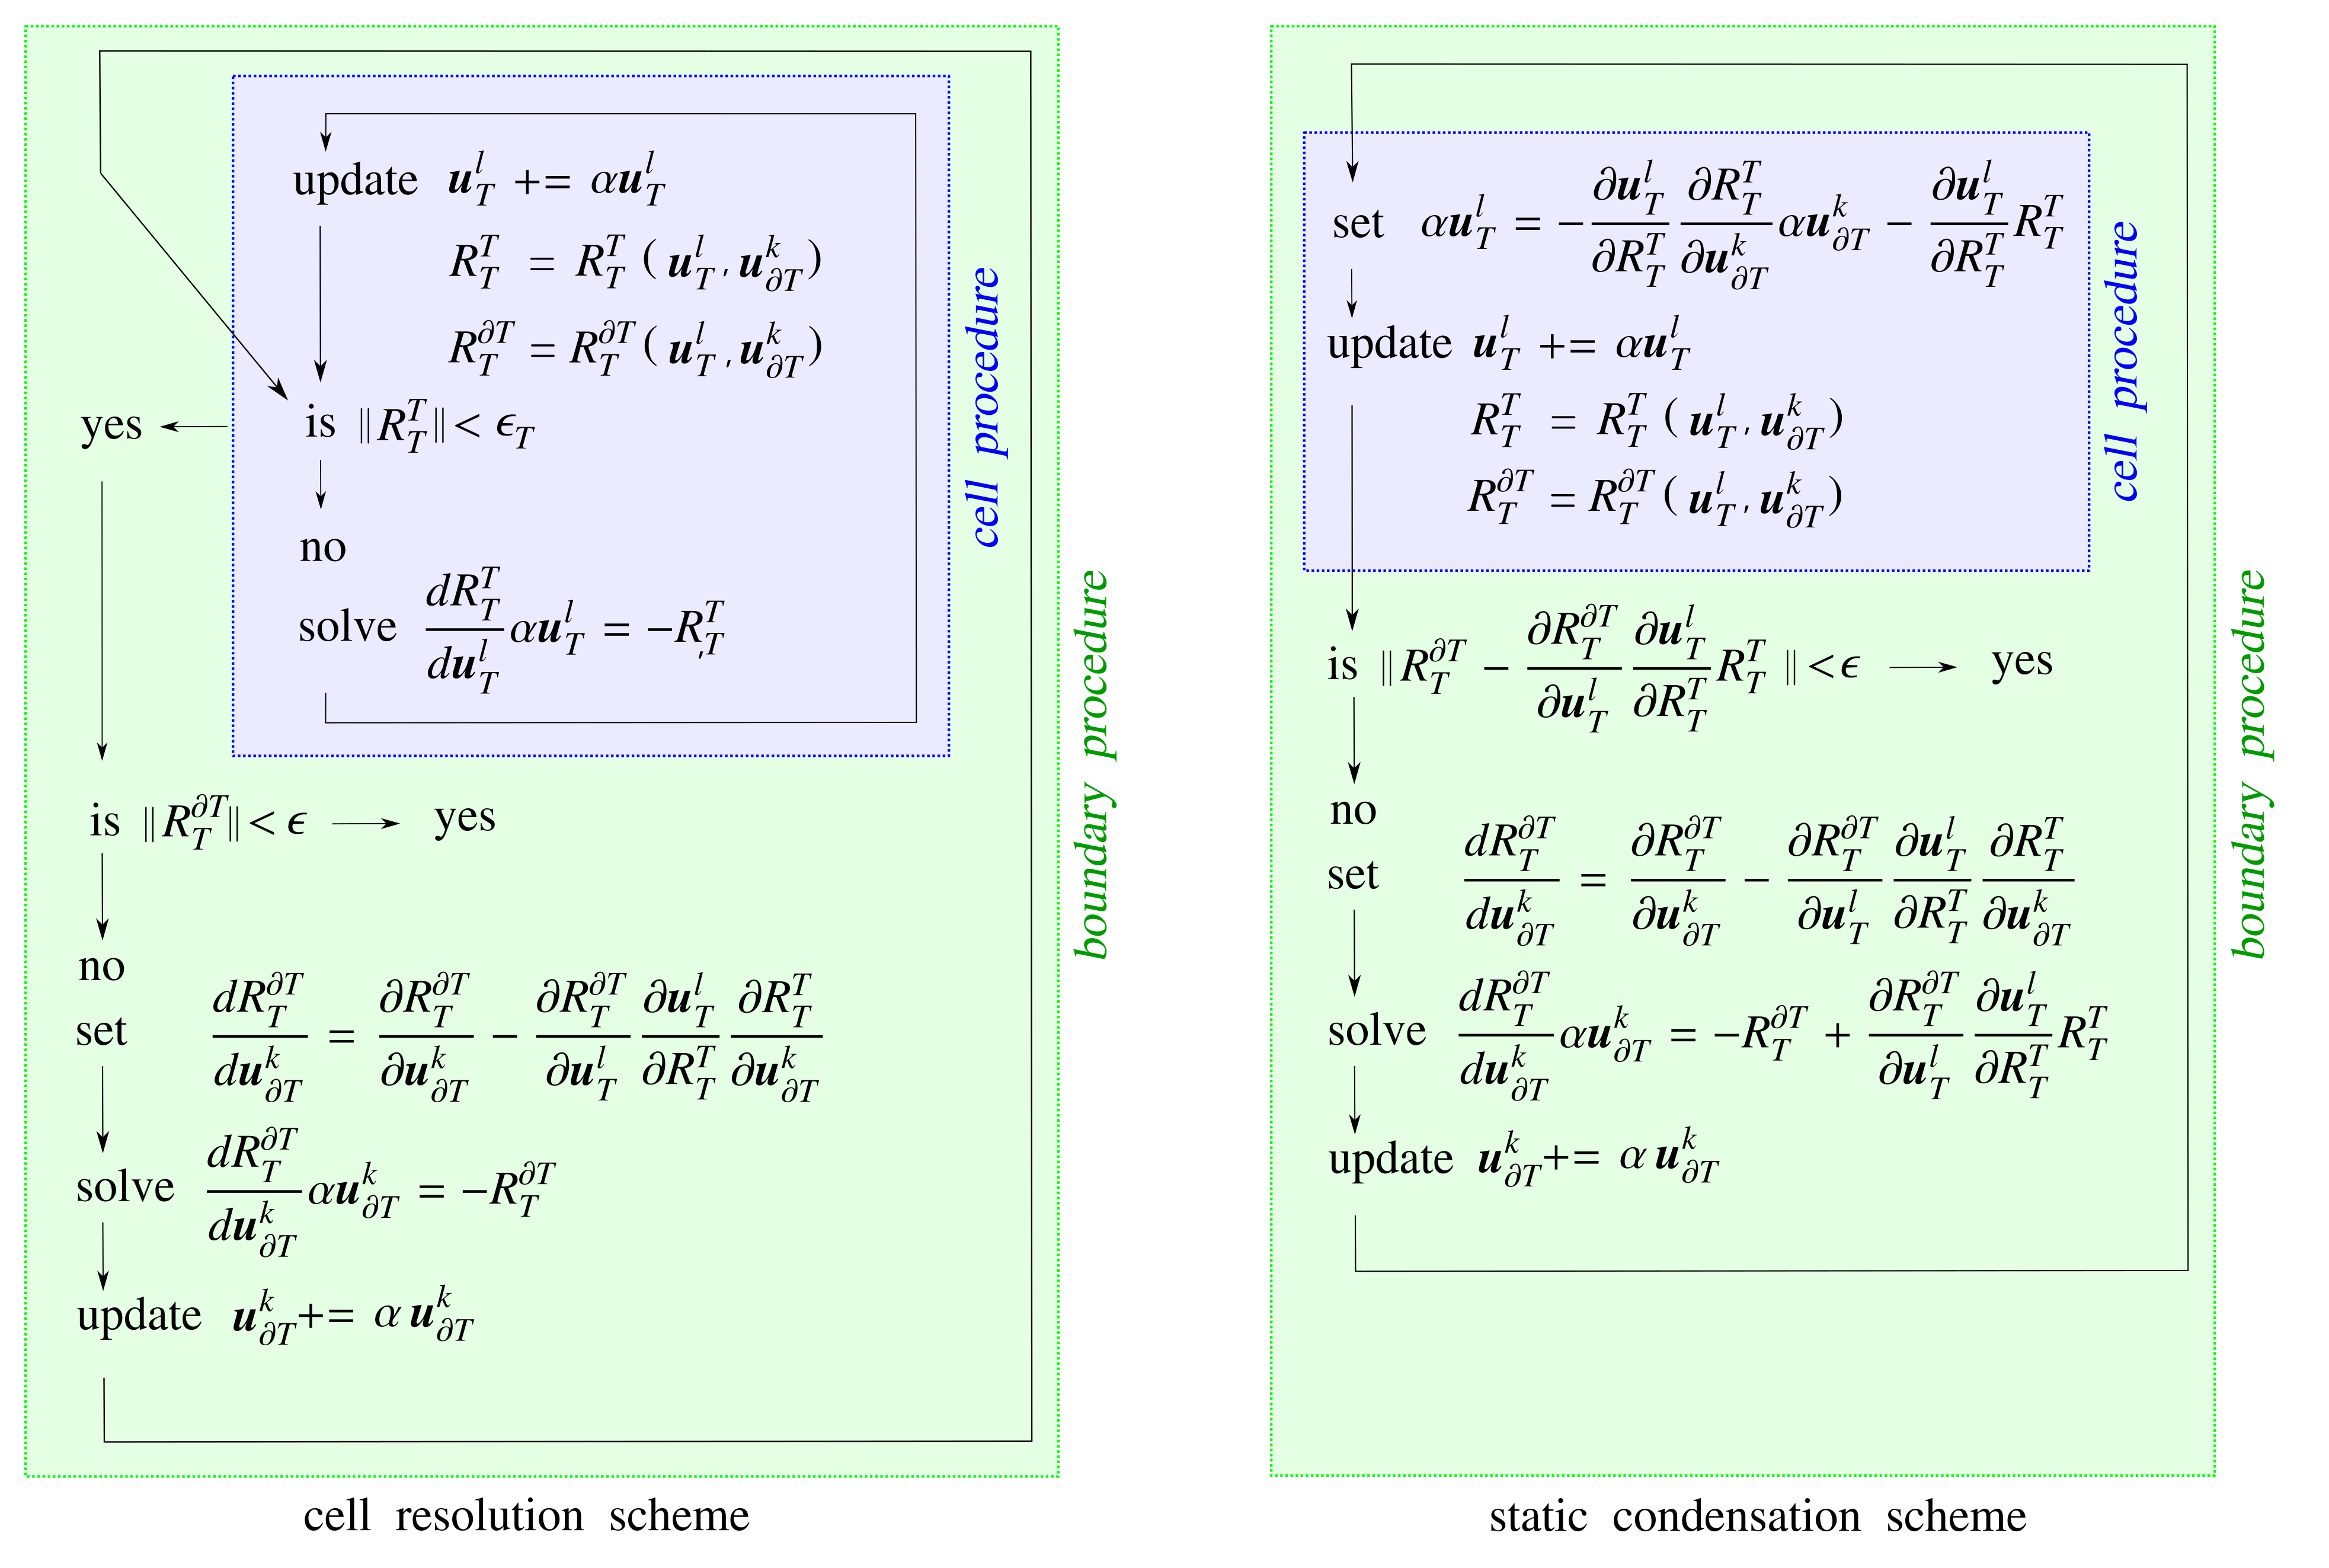
\includegraphics[width=15.cm]{chapter_002_hho_mechanics/figures/resolution.png}
%     \caption{Schematic representation of both resolution schemes}
%     \label{fig_resolution}
% \end{figure}


% NOTE : COMMENT ON TRACE LE DEPLACREMENT -> MOYENNE AU NOEUDS A PRECISER DANS LA LEGENDE DE LA FIGURE
% NOTE : LE CODE, CE QU'ON UTILISE, MFRONT MGIS -> IMPLEMENTATION PORTEE DANS CAST3M -> IMPLEMENTATION PLUGGABLE DANS AUTRE CHOSE -> 
% NOTE : ON PARLE PAS DES TEMPS DE CALCULS DANS LA SUITE parce que c du python, on montr que les 2 schémas d'intégration convergecne de manière qudartique, localement et globalement
% POUR ETRE COHERENT EN CONDENSATION, IL FAUT ACCLERER LES FACES +  LES CELLULES. POUR NOUS C QUE LES FACES


% ---------------------------------------------------------
% ---- SECTION
% ---------------------------------------------------------
\section{Numerical examples in the axisymmetric modelling hypothesis}
\label{sec_numerical_examples}

In this section, the proposed axi-symmetric HHO method is evaluated on
classical test cases taken from the literature to emphasize robustness
to volumetric locking.
The reader can refer to \ref{sec_appendix_axi} regarding technical aspects on the formulation of the proposed HHO method for the axisymmetric modelling hypothesis. 
Both the small and large strains
frameworks are considered, for elasto-plastic behaviors. The notation
HHO($k,l$) relates to the HHO element of order $k$ on faces, and order $l$ in the
cell.

The tests presented in this section have been performed using an
\texttt{python} implementation freely available on github: \url{https://github.com/davidsiedel/h2o_paper}.
The results of this implementations were thoroughly compared to the
results obtained with the reference implementation provided by the
\texttt{Disk++} solver \cite{cicuttin_implementation_2018} in the cartesian framework.

% ---------------------------------------------------------
% PARAGRAPH
% ---------------------------------------------------------
\paragraph{Stabilization parameter}

To ensure coercivity of the HHO method, the so-called \textit{stabilization} parameter
$\beta$, that relates to the Young modulus of the elastic interface introduced in Section \ref{sec_hdg_element_equilibrium}, needs be chosen according to the material under study. In \cite{di_pietro_hybrid_2015}, a value of
order $2 \mu$ is advocated, where $\mu$ denotes the shear modulus of the
material. This value is used for all test cases in the present section.

% ---------------------------------------------------------
% -- SUBSECTION
% ---------------------------------------------------------
\subsection{The free dilatation test}
\label{sec_satoh_test}

The first test case of the following benchmark aims at displaying the
robustness of the HHO method for coupled mechanical-thermal problems.

% ---------------------------------------------------------
% PARAGRAPH
% ---------------------------------------------------------
\paragraph{Specimen and loading}

For this test case, the unit box is fixed on both the right and
bottom boundaries in their respective normal directions, and a quadratic
thermal load depending on the $r$-coordinate is imposed in the solid
(see Figure \ref{fig_satoh_setting}). The mesh is composed of 400
quadrangles. The thermal loading is given by:
%
%
%
\begin{equation}
    T(r,z) = 4 (T_{max} - T_{min}) \, r \, (1 - r) + T_{min}
\end{equation}
%
%
%
with temperature values $T_{max} = 2000$ K and $T_{min} = 293.15$ K.

\begin{figure}[H]
    \centering
    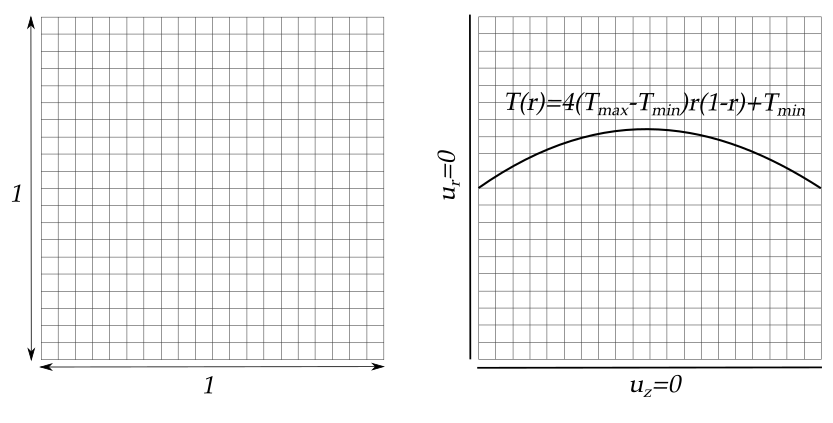
\includegraphics[width=10.cm]{../chapter_002_hho_mechanics/figures/satoh_setting.png}
    \caption{Geometry, displacement boundary conditions and temperature loading for the free dilatation test case}
    \label{fig_satoh_setting}
\end{figure}

% ---------------------------------------------------------
% PARAGRAPH
% ---------------------------------------------------------
\paragraph{Material behaviour}

A linear thermo-elastic energy potential is considered with a Young's
modulus $E$ equal to $150$ GPa. The material is quasi-incompressible
with a Poisson's ratio $\nu$ equal to $0.499$. The dilatation parameter
is taken as $\alpha = 1e^{-6}$ K$^{-1}$.

% ---------------------------------------------------------
% PARAGRAPH
% ---------------------------------------------------------
\paragraph{Volumetric locking and polynomial approximation for the strain and temperature fields}

A sign of volumetric locking is the presence of strong oscillations in the trace of the Cauchy stress (or, equivalently, the hydrostatic pressure) within elements.
Using Lagrange finite elements of order respectively $1, 2$, the
strain approximation is of order $0, 1$, whereas the thermal
strain adopted in this example is of order $2$, which results in strong signs of volumetric locking. For Lagrange
elements to accurately model the hydrostatic pressure, one needs to choose a polynomial approximation of the temperature field that is one order lower than that of the
displacement field. This feature is of major importance for mixed
elements, where quadratic displacement elements needs be employed together with linear ones for the pressure/swelling field.

\begin{figure}[H]
    \centering
    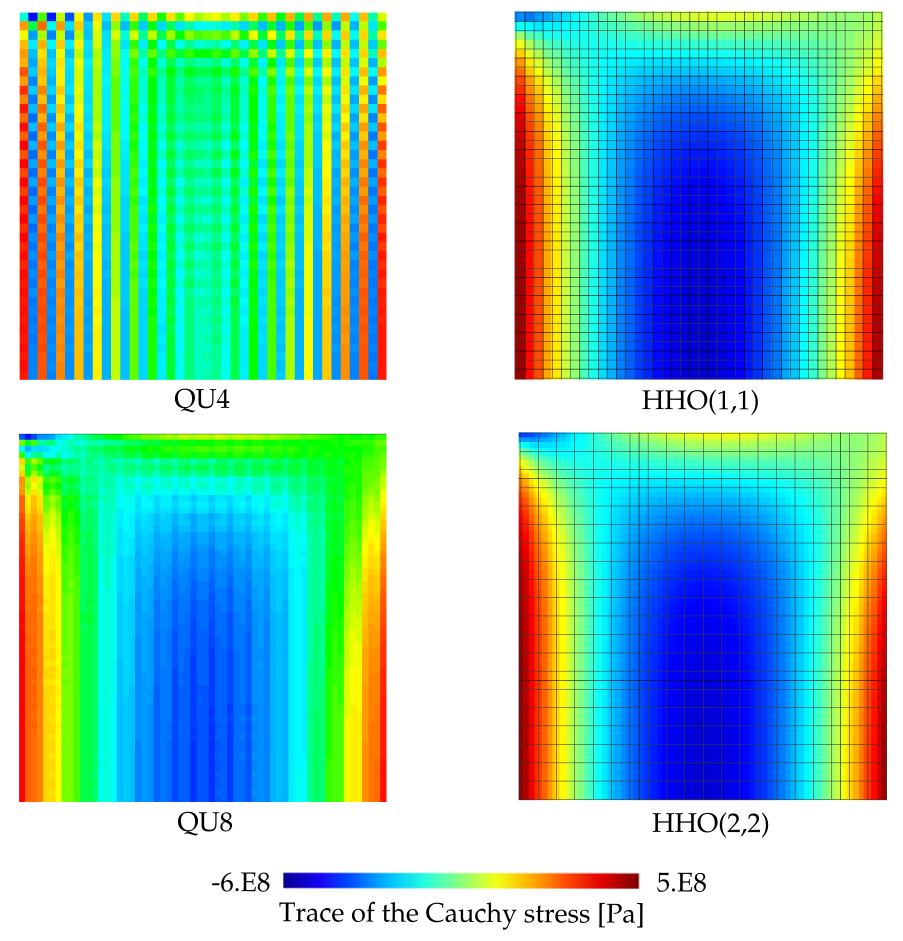
\includegraphics[width=10.cm]{../chapter_002_hho_mechanics/figures/satoh_calc.png}
    \caption{Map fo the Trace of the Cauchy stress at quadrature points for the Free dilatation test case at the last time step}
    \label{fig_satoh_calc}
\end{figure}

% ---------------------------------------------------------
% PARAGRAPH
% ---------------------------------------------------------
\paragraph{Comparison of FE and HHO methods}

In Figure \ref{fig_satoh_calc}, one can observe that the pressure map is completely smooth for HHO computations, even for a quadratic temperature field acting on a linear gradient using HHO(1,1). As expected, the results display mild signs of volumetric locking for the quadratic finite element
approximation, and strong oscillations are noted for the linear finite element solution.

% ---------------------------------------------------------
% -- SUBSECTION
% ---------------------------------------------------------
\subsection{Perfect plastic swelling sphere}
\label{sec_swelling_sphere}

% ---------------------------------------------------------
% PARAGRAPH
% ---------------------------------------------------------
\paragraph{Specimen and loading}

This benchmark consists in a quasi-incompressible sphere under uniform internal loading (see Figure \ref{fig_sphereall}).
This test case has an analytical solution and the state of the specimen is known when the plastic region has reached the external border of the sphere.
The sphere has an inner radius $r_{int} = 0.8$ mm and an outer
radius $r_{ext} = 1$ mm. An internal radial displacement $u$ is imposed.
The simulation is performed until the limit load corresponding to an internal displacement of $0.2$ mm is reached.

% ---------------------------------------------------------
% PARAGRAPH
% ---------------------------------------------------------
\paragraph{Material behaviour}

An isotropic hardening energy potential $\mecPotential{}_{\bodyLag{}}^p$ is chosen for the description of the plastic evolution of the material such that

\begin{equation}
    \mecPotential{}_{\bodyLag{}}^p(p)
    =
    \sigma_0 p + \frac{1}{2} H p^2 + (\sigma_{\infty} - \sigma_0)(p - \frac{1 - e^{-\delta p}}{\delta})
\end{equation}
%
%
%
where the parameter $p$ denotes the equivalent plastic strain and a Von Mises yields function $f$ describes the flow rule
%
%
%
\begin{equation}
    f = \sqrt{\frac{3}{2}} \rVert \text{dev} (\tensorii{\sigma}) \lVert - p
\end{equation}
%
%
%
Moreover, the small strain hypothesis is assumed, and
perfect plasticity is considered for this test case. The saturation parameter $\delta$ and the hardening parameter $H$ are taken to $0$, the yield stresses are such that $\sigma_0 = \sigma_{\infty} = 6$ MPa, and the elastic potential parameters are the Young modulus $E = 28.85$ MPa and the Poisson ratio $\nu = 0.499$, such that the material is quasi-incompressible.

\begin{figure}[H]
    \centering
    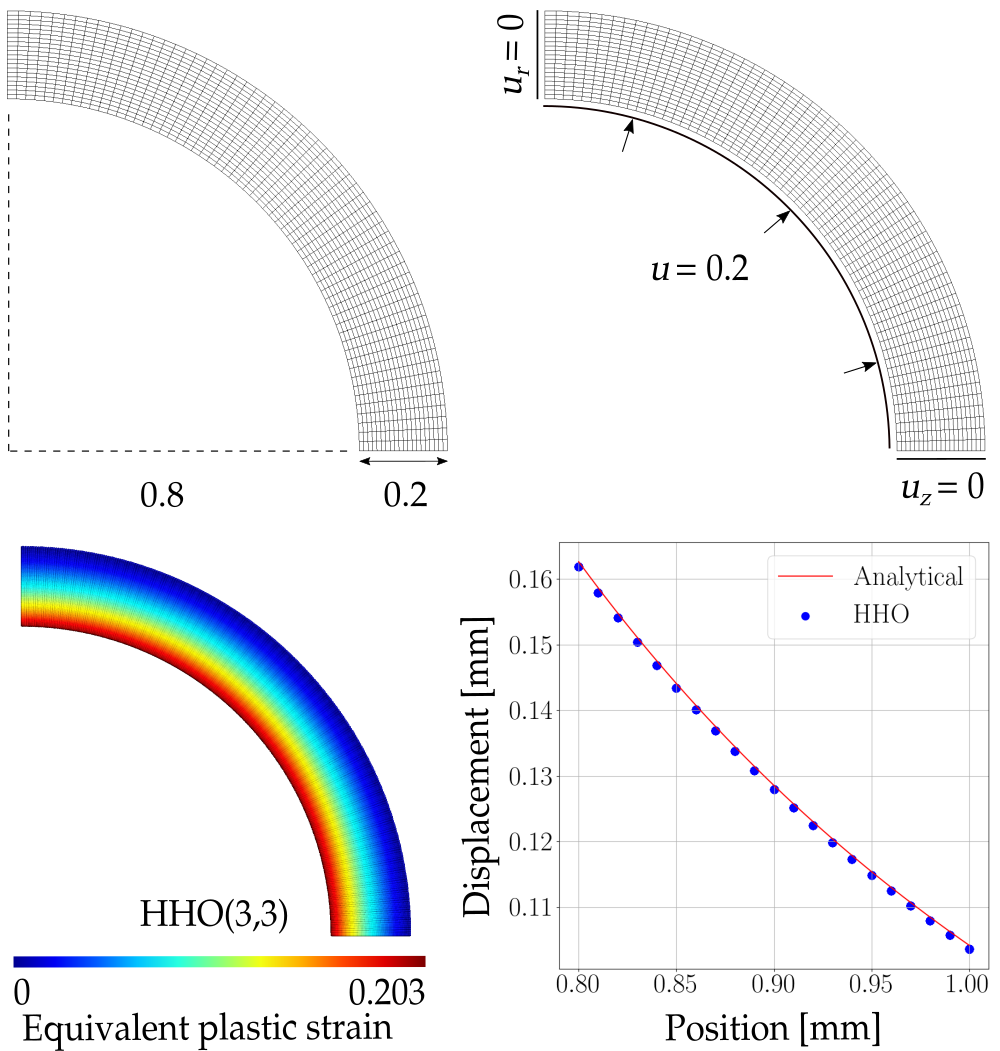
\includegraphics[width=12.cm]{../chapter_002_hho_mechanics/figures/sphere_mesh.png}
    \caption{the swelling sphere test case. Geometry, loadings, final displacement along the radius of the sphere, and final equivalent plastic strain map at quadrature points}
    \label{fig_sphereall}
\end{figure}

% ---------------------------------------------------------
% PARAGRAPH
% ---------------------------------------------------------
\paragraph{Displacement along the radius}

Since an analytical solution is known for this test case, it is compared to the proposed HHO method numerical results. The displacement of the section of the sphere at cell nodes
is plotted in Figure \ref{fig_sphereall}, along with the analytical one, and it is noticed that the obtained results are in agreement with the analytical ones.
Figure \ref{fig_sphereall} mentions the label HHO without specifying approximation orders for all computations deliver the same result.

% ---------------------------------------------------------
% PARAGRAPH
% ---------------------------------------------------------
\paragraph{Trace of the Cauchy stress}

As for the displacement, the analytical solution for the trace of the Cauchy stress tensor is compared to the one computed using the proposed HHO method for three approximation orders.
Numerical results at quadrature points fit the analytical curve, and display no sign of volumetric locking. The computed solution is however less smooth
at the borders of the specimen for higher orders, a phenomenon that was pointed out in \cite{abbas_hybrid_2019-1} for the three dimensional case, and attributed to the fact that planar faces are considered.

\begin{figure}[H]
    \centering
    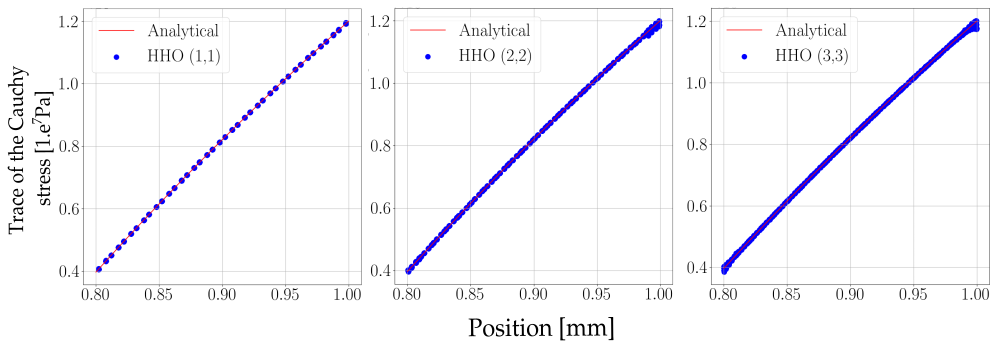
\includegraphics[width=15.cm]{../chapter_002_hho_mechanics/figures/sphere_pressures.png}
    \caption{trace of the Cauchy stress tensor along the radius of the sphere at quadrature points}
    \label{fig_sphere_pressure}
\end{figure}

% ---------------------------------------------------------
% -- SUBSECTION
% ---------------------------------------------------------
\subsection{Necking of a notched bar}

% ---------------------------------------------------------
% PARAGRAPH
% ---------------------------------------------------------
\paragraph{Specimen and loading}

The last application consists of a notched bar that is subjected to uniaxial
extension.
The bar has a length of $30$ mm, a top section of radius $5$ mm and a bottom section of radius $3$ mm.
A vertical
displacement $u_z = 0.8$ mm is imposed at the top, as shown in Figure \ref{fig_ssnaallmesh}.
For symmetry reasons, only one-quarter of the
bar is discretized.

% ---------------------------------------------------------
% PARAGRAPH
% ---------------------------------------------------------
\paragraph{Behaviour law}

The same behavior law as that in \ref{sec_swelling_sphere} is considered for the present test case. 
However, the finite strain hypothesis is chosen, based on a logarithmic decomposition of the stress \cite{miehe_anisotropic_2002}.

% ---------------------------------------------------------
% PARAGRAPH
% ---------------------------------------------------------
\paragraph{Material parameters}

Materials parameters are taken as
$\sigma_0 = 450$ MPa, $\sigma_{\infty} = 715$ MPa with a saturation parameter $\delta = 16.93$. The Young modulus is $E = 206.9$ GPa, and the Poisson ratio is $\nu = 0.29$.

% ---------------------------------------------------------
% PARAGRAPH
% ---------------------------------------------------------
\paragraph{Load deflection curve}

The load-displacement curve is plotted
in Figure \ref{fig_ssnaallmesh}, and gives similar results to that obtained with quadratic reduced integration elements.

% ---------------------------------------------------------
% PARAGRAPH
% ---------------------------------------------------------
\paragraph{Equivalent plastic strain}

Moreover, the equivalent
plastic strain $p$ at quadrature points and at the final load is plotted Figure \ref{fig_ssnaallplastic}.
It has been observed that the equivalent plastic strain might suffer some oscillations at a certain limit load with UPG methods.
One notices through the present example, that the proposed HHO method displays no oscillations of the equivalent plastic strain.

\begin{figure}[H]
    \centering
    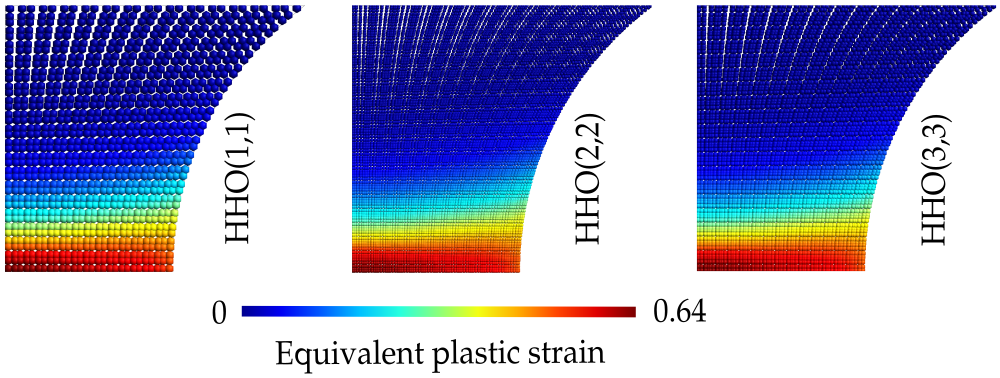
\includegraphics[width=12.cm]{../chapter_002_hho_mechanics/figures/ssna_plastic.png}
    \caption{
        final equivalent plastic strain map at quadrature points in the notch region
    }
    \label{fig_ssnaallplastic}
\end{figure}

% ---------------------------------------------------------
% PARAGRAPH
% ---------------------------------------------------------
\paragraph{Hydrostatic pressure}

The hyrostatic pressure map at quadrature points and at the final load is shown Figure \ref{fig_ssnaallmesh} for three HHO element orders (respectively $1, 2$ and $3$).
As for the swelling sphere test case, one notices that the hydrostatic pressure map is
fairly smooth over the whole structure at all approximation orders, even at the bottom left corner where plasticity is confined.

\begin{figure}[H]
    \centering
    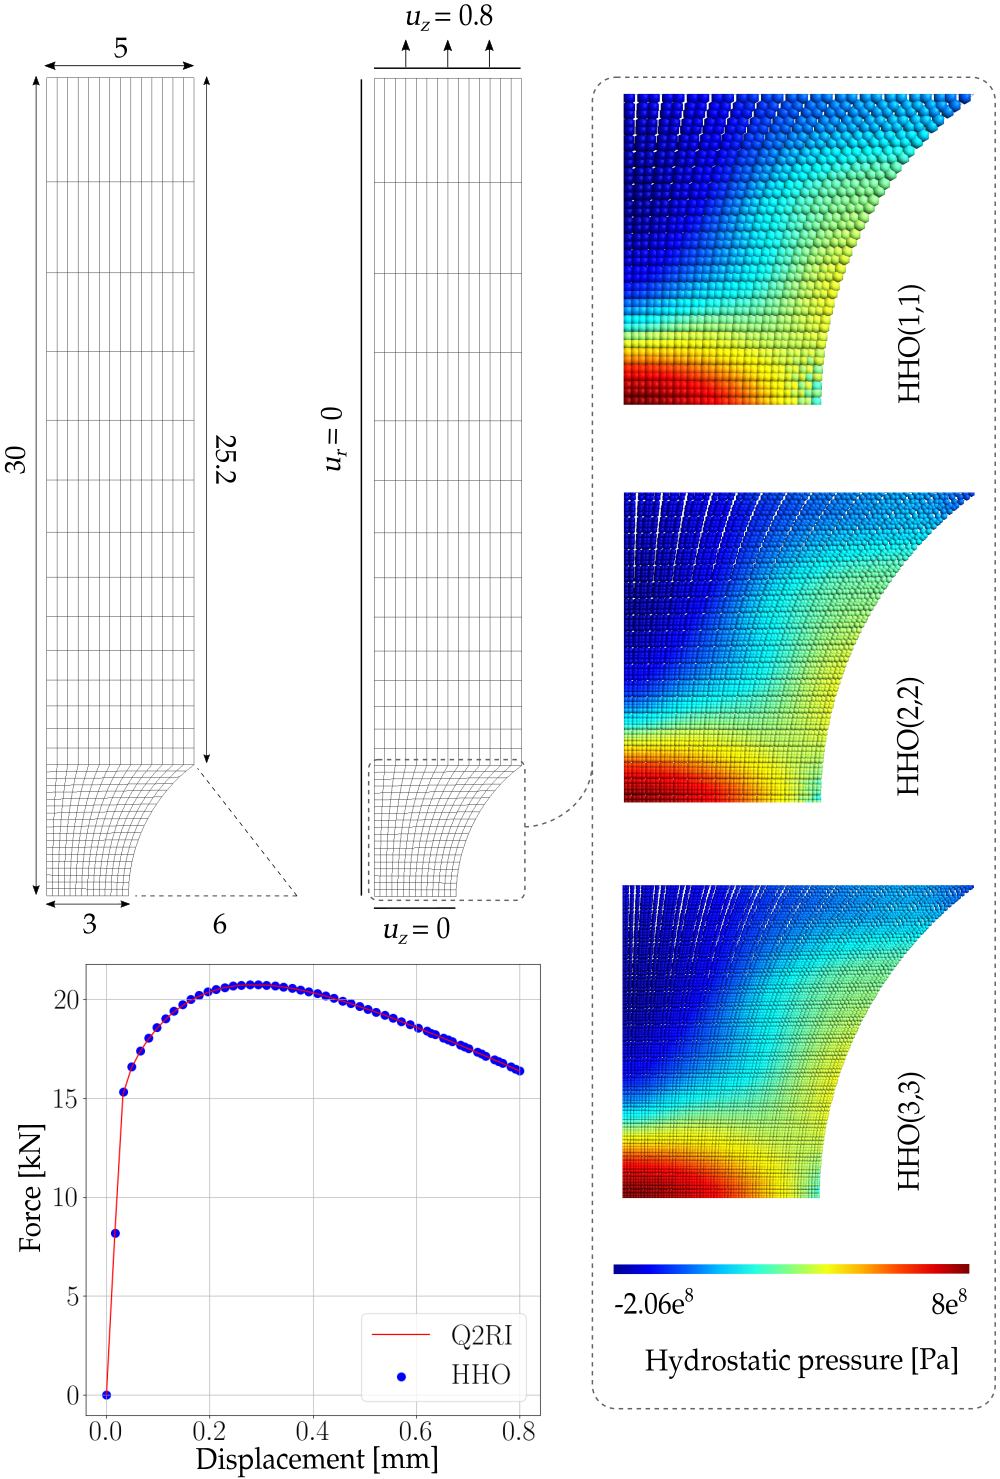
\includegraphics[width=12.cm]{../chapter_002_hho_mechanics/figures/ssna_mesh.png}
    \caption{
        the notched specimen test case. Geometry, loadings, load deflection curve, and final hydrostatic pressure map at quadrature points in the notch region
    }
    \label{fig_ssnaallmesh}
\end{figure}

% ---------------------------------------------------------
% ---- SUBSECTION
% ---------------------------------------------------------
\subsection{Comparison of cell unknowns elimination schemes}
\label{sec_num_example_part_2}

In this section, both elimination strategies
introduced in Section \ref{sec_cell_unknowns_elimination} are evaluated. In particular, four different variants of the usual
Newton algorithm
are studied, namely :
% \begin{itemize}
%     \item (R) the Static condensation scheme using a consistent Jacobian operator
%     \item (M1) the Cell equilibrium scheme using a consistent Jacobian operator
%     \item (M2) the Static condensation scheme using an elastic Jacobian operator
%     \item (M3) the Cell equilibrium scheme using an elastic Jacobian operator
%     \item (M4) the Static condensation scheme using an elastic Jacobian operator and coupled with an Anderson acceleration algorithm, that acts on both cell and faces unknowns at the global level
%     \item (M5) the Cell equilibrium scheme using an elastic Jacobian operator coupled with an Anderson acceleration algorithm on faces unknowns only
% \end{itemize}
(Sc) a Static condensation scheme using a consistent Jacobian operator,
(Cc) a Cell equilibrium scheme using a consistent Jacobian operator,
(Se) a Static condensation scheme using an elastic Jacobian operator,
(Ce) a Cell equilibrium scheme using an elastic Jacobian operator,
(Sa) a Static condensation scheme using an elastic Jacobian operator and coupled with an Anderson acceleration algorithm, that acts on both cell and faces unknowns at the global level,
(Ca) a Cell equilibrium scheme using an elastic Jacobian operator coupled with an Anderson acceleration algorithm on faces unknowns only.

The last two test cases that showcase non-linear behaviours are considered for the evaluation of all these variants. The static condensation resolution scheme that uses a consistent stiffness matrix is taken for reference, since it is the
one used in the literature \cite{abbas_hybrid_2019,abbas_hybrid_2018}.
The estimation of the Anderson acceleration is performed every iteration and is based on the last three residual and unknown vectors.

\paragraph{Number of iterations per time step}

The number of iterations per time step for each variant
is displayed in Figure \ref{fig_acceleration_res_0} for both the swelling sphere test case
and the notched rod one.
At each time steps, the number of iteration is normalized by the number of iterations obtained with the
Static condensation variant (Sc).
As expected, the number of iteration per time step is similar for Cell resolution scheme based variants and Static condensation ones, for all polynomial orders and all alternatives listed above.

\begin{figure}[H]
    \centering
    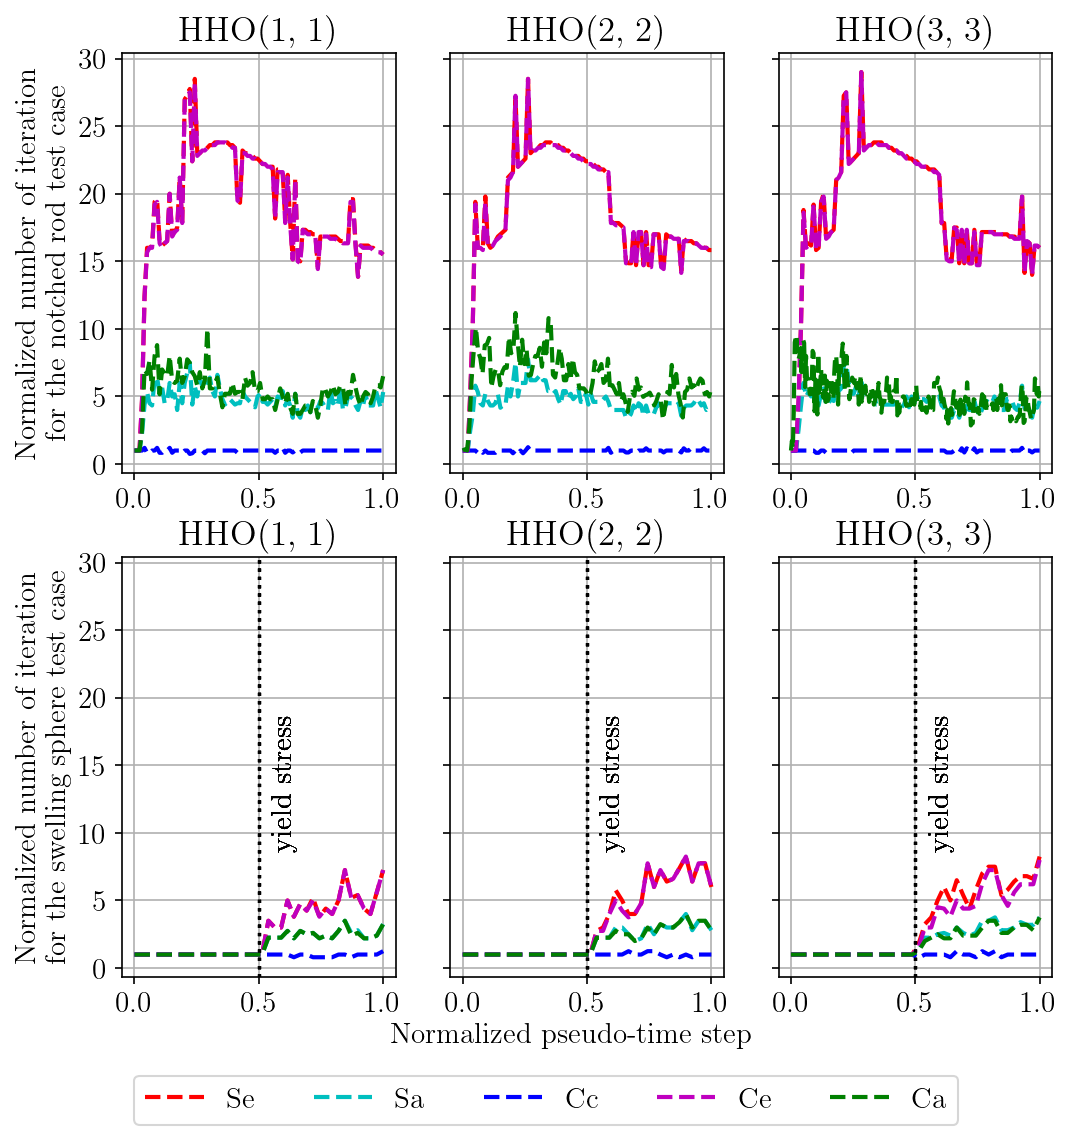
\includegraphics[width=12.cm]{../chapter_002_hho_mechanics/figures/plot_global_iterations__4_ordn.png}
    \caption{Normalized number of iterations per time step for non-linear test cases and all resolution schemes variants}
    \label{fig_acceleration_res_0}
\end{figure}

\paragraph{Accelereated variants comparison}

The key argument in using the
Cell equilibrium scheme with an acceleration step is that 
only faces unknowns are accelerated.
Using the static condensation scheme demands to accelerate both cell and faces unknowns simultaneously.
However, using the Cell equilibrium scheme, the update of the cell unknown after a sole face acceleration step is performed at the cell level.
From a mechanical standpoint, faces unknowns are perturbed, and solving non-linear equation \eqref{eq_cell_equilibrium_1} by a local Newton algorithm as depicted in Section \ref{sec_cell_equilibrium_scheme} allows to retrieve the cell unknown increment verifying the equilibrium of the element.

\paragraph{Memory footprint}

In addition, local matrices used for the decondensation step in the Static condensation scheme are not kept from one iteration
to another using the Cell equilibrium scheme, hence drastically reducing the total memory footprint of the computation.
The number of scalar values to be stored between each iteration for a cell $\cell$ and for each variant is given in Table \ref{table_memory_footprint}, where $d$ is the number of components of the unknown field,
$M^l_T$ is the size of a scalar cell polynomial unknown, $M^l_T$ is that of a face, $N_{\dCell}$ is the number of faces for the cell $T$, and
$N_{it}$ denotes the number of residual and associated unknowns to be stored by the Anderson acceleration algorithm.

\begin{table}[H]
    \centering
    \begin{tabular}{||c c||} 
        \hline
        Resolution Method & Memory footprint
        \\
        [0.5ex] 
        \hline\hline
        (Sc), (Se) & $d \, M^l_T (M^k_{\dCell} \, N_{\dCell} + M^l_T)$
        \\ \hline
        (Cc), (Ce) & 0
        \\ \hline
        (Sa) & $d \, M^l_T (M^k_{\dCell} \, N_{\dCell} + M^l_T) + d \, 2 \, N_{it} (M^k_{\dCell} \, N_{\dCell} + M^l_T) $
        \\ \hline
        (Ca) & $d \, 2 \, N_{it} (M^k_{\dCell} \, N_{\dCell})$
        \\ \hline
    \end{tabular}
    \caption{Memory footprint for each alternative and for an element}
    \label{table_memory_footprint}
\end{table}

The number of scalar values that need be stored from one iteration to another for a single quandrangular element, depending on the discretization, and on the chosen acceleration scheme (\textit{i.e.} on the number of resiudal and unknown vectors to store)
is given in Figure \ref{fig_acceleration_res_memory} for different acceleration strategies, cell and faces polynomial orders.

\begin{figure}[H]
    \centering
    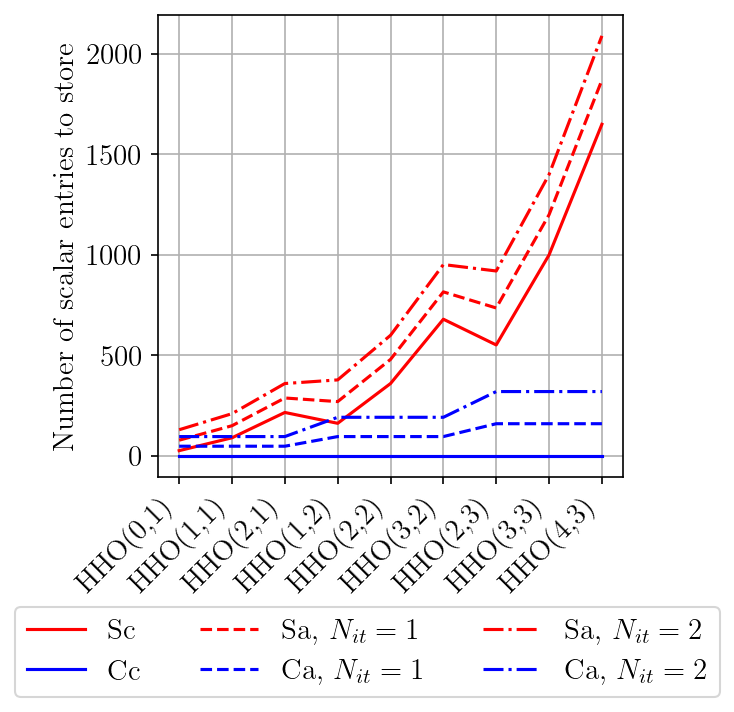
\includegraphics[width=8.cm]{../chapter_002_hho_mechanics/figures/plot_memory.png}
    \caption{Number of scalar entries to store from one iteration to another for different polynomial orders and resolution schemes variants}
    \label{fig_acceleration_res_memory}
\end{figure}

\paragraph{Local iterations}

The price for alleviating the memory footprint of the Static condensation scheme
is paid by systematic calls to the local Newton algorithm.
As a consequence, one also notices an increasing number of calls to the behaviour law.
The mean number of local cell iterations per time time step is given in Figure \ref{fig_acceleration_res_1} for both test cases. The high number of cell iterations for the swelling sphere test case is
due to the fact that the plastic front involves a linearly increasing number of cells submitted to a perfect plastic beahviour.
Considering \textit{e.g.} a linear hardening behaviour law leads to a stabilized number of cell iterations once the whole domain is plastic.

\begin{figure}[H]
    \centering
    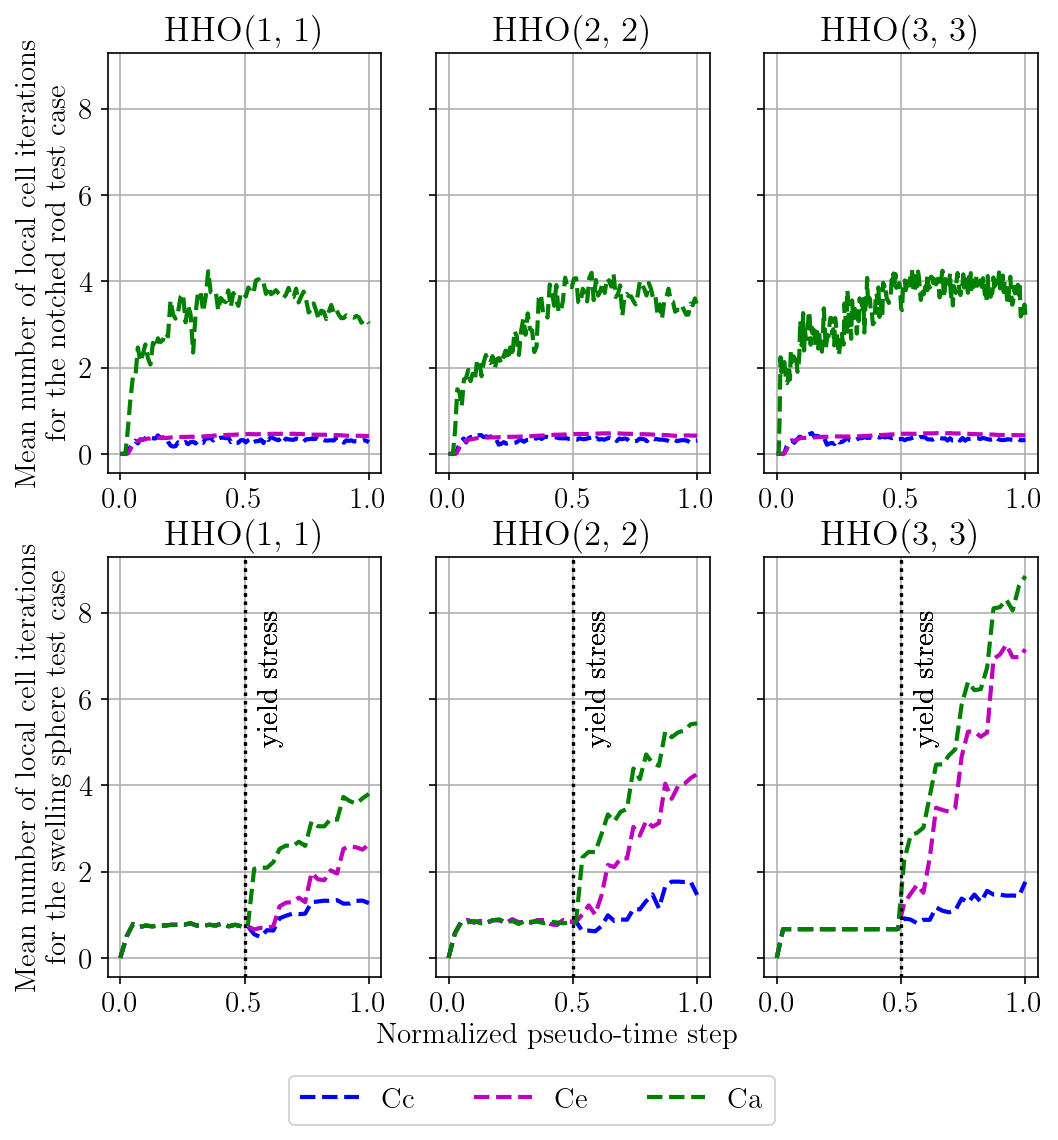
\includegraphics[width=12.cm]{../chapter_002_hho_mechanics/figures/plot_cell_iterations__4_cell_iters.png}
    \caption{Normalized number of cell iterations per time step for non-linear test cases and Cell equilibrium based resolution schemes variants}
    \label{fig_acceleration_res_1}
\end{figure}

\paragraph{Local system}

The local system to solve with each cell scales with the size of a single cell unknown. An overview of the values taken using a monomial shape function can be found in \ref{sec_appendix_implementation}. These local resolution procedures consist in solving dense systems and are completely
parallelizable.

% \subsubsection{Quadratic and accelerated schemes}

% Both the Cell equilibrium and Static condensation resolution schemes are compared in terms of number of global iterations, using either
% a consistent stiffness matrix, an elastic operator, and an elastic operator coupled with an Anderson acceleration
% algorithm.
% The static condensation resolution scheme that uses a consistent stiffness matrix is taken for reference, since it is the
% one used in the literature \cite{abbas_hybrid_2019,abbas_hybrid_2018}.

% \paragraph{Resolution schemes using a consitent stiffness matrix}

% The number of iterations per time step for the Cell equilibrium algorithm using a consistent tangent operator
% is showcased by the dashed blue line in Figure \ref{fig_acceleration_res_0} for the swelling sphere test case,
% and in Figure \ref{fig_acceleration_res_1} for the notched rod one.
% Results are normalized by those obtained with the Static condensation algorithm.
% As expected, the number of iteration per time is roughly the same between the Cell resolution scheme
% and the Static condensation one, for all polynomial orders.

% \paragraph{Resolution schemes using an elastic stiffness matrix}

% Keeping the first elastic stiffness matrix for the whole computation showcases assets that are discussed in Section \ref{sec_cell_unknowns_elimination}. In this section, four resolution methods based on the elastic stiffness matrix are studied :
% \begin{itemize}
%     \item (M1) the Static condensation scheme
%     \item (M2) the Cell equilibrium scheme
%     \item (M3) the Static condensation scheme, coupled with an Anderson acceleration algorithm, that acts on both cell and faces unknowns at the global level
%     \item (M4) the Cell equilibrium scheme, coupled with an Anderson acceleration algorithm on faces unknowns only
% \end{itemize}
% %
% %
% %
% The number of iterations 
% (M1) the Static condensation scheme, (M2) the Cell equilibrium scheme, (M3) the Static condensation scheme, coupled with
% an Anderson acceleration algorithm, that acts on both cell and faces unknowns at the global level and (M4) the Cell
% equilibrium scheme, coupled with an Anderson acceleration algorithm for faces unknowns only.

% \paragraph{}

% Figure \ref{fig_acceleration_res_0} gives the number of iterations needed to achieve convergence
% at the skeletal level, with respect to the current pseudo-time step. The computation is performed
% in $40$ uniform steps from an initial steady state up to the limit radial load of $0.2$ mm (see \ref{sec_swelling_sphere}).
% For this experiment, three variants of both cell elimination schemes are considered :
% \begin{itemize}
%     \item A first scheme S1 consists in using a consistent tangent operator for the computation of the stiffness matrix
%     \item A second scheme S2 consists in using an elastic tangent operator for the computation of the stiffness matrix
%     \item A last scheme consists in us
% \end{itemize}

% ---------------------------------------------------------
% ---- SECTION
% ---------------------------------------------------------
\section{Conclusion}

% Dire de maniere explicte, mettre les éléments virtuels dans le même cadre -> dire quil reste à examiner le lien avec les éléments viertuels 
% Le HW permet de retrouver les principes HDG, HHO qui sont au coeur de ce paprier mais aussi les cG
% les VEM notn pas ete bconsideres, bien que le cadrez propos semblke sadapter à leur formalmisme
% descxirption du code, trouvaable sur github, avec chaque exemple

An introduction to HDG and HHO methods has been proposed, based on the minimization of a Hu-Washizu Lagrangian. The expression of the method arising from this approach allows to introduce naturally all the ingredients of the method, as well as the displacement discontinuity, in a unified framework.
This formulation also allows to draw a connection between HDG methods and other locking-free methods based on the minimization of a Hu-Washizu Lagrangian.
A natural cell-based resolution scheme emerged from this formulation, that has been tested and evaluated.
Finally, a HHO method to account for mechanical problems in the axisymmetric framework has been devised and evaluated numerically, for both linear thermoelastic behaviours, and plastic behaviours under both the small and finite strain hypotheses.
The proposed HHO method exhibits a robust behaviour to volumetric locking for strain-hardening plasticity as well as for perfect plasticity in primal formulation, with a moderate number of degrees of freedom.

This work can be pursued in several directions. One could use the cell resolution algorithm to address local resolution problems, such as those encountered with \textit{e.g.} damage irreversibility in phase field fracture mechanics, or multi field plasticity. Moreover, an adaptation of the HHO method to
reconstruct pressure-driven gradient terms only could lead to a simpler formulation, closer to that of mixed methods \cite{simo_quasi-incompressible_1991}.

\chapter{Micromorphic damage behaviours for quasi-brittle materials}
\label{chapter:micromorphic_damage}

\section{Introduction}

The variational approach to fracture takes its grounds in the work of
Francfort and Marigo which recasted the Griffith theory into an enery
minimization problem \cite{francfort_revisiting_1998,francfort_vers_2002}.
This revisted approach of the Griffith theory is however not tractable
with standard numerical methods
\cite{bourdin_numerical_2000,chambolle_approximation_2018}, in particular
the commonly used finite element method. For this reason, Bourdin *et
al.* developed regularised versions \cite{bourdin_numerical_2000} following
the works of Ambrosio and Tortorelli \cite{ambrosio_approximation_1990}.

The so-called phase-field approaches to fracture have since become
widely popular. As pointed by Gerasimov and De Lorenzis in their
excellent review \cite{gerasimov_numerical_2020}, one of the main
difficulties in the implementation of those approaches is the treatment
of the irreversibility constraint (the damage can only increase), a
question on which a considerable amount of works has been published.
Most of the proposed solutions are not directly implemented in standard
FEM or FFT solvers. An noticeable exception to this statement is the
Miehe' alternative based an the so-called history variable
\cite{miehe_phase_2010}. However, Miehe' alternative is not variationally
consistent.

Following Forest' micromorphic framework
\cite{forest_micromorphic_2009,forest_nonlinear_2016}, we propose in
Section \ref{sec:micromorphicdamage:description}a class of micromorphic
brittle behaviours which can approximate classical models of britle
fracture in a variationnally consistent way. These behaviours allow to
deal with the irreversibility constraint at integration points,
instead of having to deal with it in the solution of balance equation. Such
advantages have been highlighted by Rezaee-Hajidehi et al. in the
context of phase-field approaches to phase transformation
\cite{rezaee-hajidehi_micromorphic_2021}. The balance equations are
standard partial differential equations which can readily be solved by
most FEM or FFT solvers.

Such micromorphic models were recently investigated by Bharali \textit{et al.}
\cite{bharali_computational_2021} to approximate the AT1 and AT2 models
using a monolithic resolution strategy. In this paper, we exploit the
variational basis of the behaviour to derive in Section
\ref{sec:micromorphicdamage:alternate_minimisation}three alternate
minimization schemes whose convergence is guaranteed.

Several test cases comparing the prediction of the classical AT2 model
and its micromorphic counterpart are presented in Section
\ref{sec:micromorphicdamage:test_cases}.
The choice of the penalisation
parameter is discussed in-depth.

Two numerical experiments are presented in Section
\ref{sec:micromorphicdamage:numerical_experiments}, which assess:

\begin{itemize}
    \item The performance of the micromorphic approach with high order finite
    elements in the case of shear driven fracture.
    The scalability of the micromorphic approach.
\end{itemize}

\subsection{Description of the micromorphic behaviours}
\label{sec:micromorphicdamage:description}

In this paper, we consider the quasi-static evolution of a body
\(\Omega\) made of a brittle material.

The state of this material is characterized, at each time step, by:

\begin{itemize}
    \item A displacement field $\DisplacementField$.
    \item A micromorphic damage field $\MicromorphicDamageField$.
    \item A local damage field $\DamageField$.
\end{itemize}

In the view of simple generalized standard materials
\cite{moreau_sur_1970,halphen_sur_1975,ehrlacher_principe_1985,nguyen_standard_2002},
the micromorphic model is defined by the following incremental
Lagrangian \cite{lorentz_variational_1999,forest_localization_2004}:
%
%
%
\begin{equation}
  \label{eq:ef_micromorphic:formulation:total_lagrangian}
  \LagrangianOperator{\BodyLagrange}{}(\DisplacementField, \DamageField, \MicromorphicDamageField)
  =
  \int_{\BodyLagrange} \FreeEnergy_{\BodyLagrange}(\SmallStrainField, \DamageField, \MicromorphicDamageField, \nabla \MicromorphicDamageField)
  +
  \int_{\BodyLagrange} \Delta t \, \Dissipation_{\BodyLagrange} \paren{\frac{\DamageField - \bts{\DamageField}}{\Delta t}}
  -
  \int_{\BodyLagrangeNeumannBoundary} \neumannLag \cdot \DisplacementField
\end{equation}
%
%
%
where:
%
%
%
\begin{itemize}
    \item \(\FreeEnergy_{\BodyLagrange}\) is the free energy.
    \item \(\Dissipation_{\BodyLagrange}\) is the dissipation potential.
    \item \(\Delta\,t\) is the time increment.
    \item \(\bts{\DamageField}\) is damage at the beginning of the time step.
    \item \(\neumannLag\) is the imposed traction on the boundary \(\partial\,\Omega_{T}\).
    \item \(\DisplacementField, \DamageField, \MicromorphicDamageField\) denotes any admissible displacement, damage and micromorphic damage field.
    \item \(\BodyLagrangeNeumannBoundary\) is the part on the boundary where external reaction forces are imposed
\end{itemize}
%
%
%
To satisfy the Ilyushin-Drucker postulate, the incremental Lagragian
\(\mathcal{L}\) must be convex with respect to each variables
\(\vec{u}^{\star},d^{\star},d_{\chi}^{\star}\) taken independently. It
can be shown that this condition is ensured if the \(\freeenergy\) and
the dissipation potential \(\dissipationpotential\) are convex with
respect to their respective arguments.

\paragraph{Body forces and prescribed micromorphic tractions}

The definition of the Lagrangian \(\mathcal{L}\) can be enriched by adding
body forces (such as gravity) and prescribed micromorphic tractions.

The state of the material minimizes the incremental Lagrangian:
\begin{equation}
  \label{eq:ef_micromorphic:formulation:total_lagrangian_min}
  \paren{\ets{\vec{u}}, \ets{d_{\chi}}, \ets{d}} = \underset{\vec{u}^{\star}\in C.A.}{\argmin}\, \mathcal{L}\paren{\vec{u}^{\star},d^{\star},d_{\chi}^{\star}}
\end{equation}
% \[
% \paren{\ets{\vec{u}}, \ets{d_{\chi}}, \ets{d}} = \underset{\vec{u}^{\star}\in C.A.}{\argmin}\, \mathcal{L}\paren{\vec{u}^{\star},d^{\star},d_{\chi}^{\star}}
% \]

In practice, the free energy is a differentiable function.

This is not the case for the dissipation potential
\(\dissipationpotential\) for time independent mechanisms for which
\(\dissipationpotential\) is assumed to be an homogeneous function of
degree \(1\). Consequently, this which allows to eliminate the time increment
\(\Delta\,t\) from the definition of the Lagrangian such that :
\begin{equation}
  \label{eq:ef_micromorphic:formulation:dissipation}
  \Delta\,t\,\dissipationpotential\paren{\Frac{d^{\star}-\bts{d}}{\Delta\,t}} = \dissipationpotential\paren{d^{\star}-\bts{d}}
\end{equation}
% \[
% \Delta\,t\,\dissipationpotential\paren{\Frac{d^{\star}-\bts{d}}{\Delta\,t}} = \dissipationpotential\paren{d^{\star}-\bts{d}}
% \]

In particular, the dissipation potential generally contains an indicator
function imposing the \textit{irreversibility of the damage evolution}.

\subsubsection{Equilibrium}

Deriving equilibrium equations from the principle of the minimum of the
Lagrangian is non trivial due to the fact that the dissipation potentiel
is not differentiable.
%
%
%
It is then convenient to separate the Lagrangian into two parts
\(\mathcal{L}_{1}\) and \(\mathcal{L}_{2}\) as follows:
%
%
%
\begin{subequations}
  \label{eq:ef_micromorphic:formulation:total_lagrangian_split}
      \begin{alignat}{3}
        \mathcal{L}_{1}\paren{\vec{u}^{\star},d^{\star},d_{\chi}^{\star}}
        &
        = 
        \int_{\Omega} \freeenergy\paren{\tepsilon^{\star}, d^{\star}, d_{\chi}^{\star},\nabla\,d_{\chi}^{\star}} \,\dtot\,V
        -
        \int_{\partial\,\Omega_{T}} \vec{T}\,\cdot\,\vec{u}^{\star} \,\dtot\,S
        \label{eq:ef_micromorphic:formulation:total_lagrangian_split:eq0}
        \\
        \mathcal{L}_{2}\paren{d^{\star}}
        &
        = 
        \int_{\Omega}
        \dissipationpotential\paren{d^{\star}-\bts{d}}
        \,\dtot\,V
        \label{eq:ef_micromorphic:formulation:total_lagrangian_split:eq1}
  \end{alignat}
\end{subequations}

In this report, the following mathematical result characterizing
the minima of Lagrangian \cite{son_standard_2021} are assumed :

\begin{itemize}
    \item The regular part of the Lagrangian \(\mathcal{L}_{1}\) is minimal with
    respect to the displacement field \(\vec{u}\) and the micromorphic
    damage field \(d_{\chi}\).
    \item At each point, the thermodynamic force \(Y\) associated with the
    damage, is in the subgradient of the dissipation potential:
    \begin{equation}
      \label{eq:ef_micromorphic:formulation:generalized_standard_0}
      Y \in \partial \dissipationpotential
    \end{equation}
    % \[
    % Y \in \partial \dissipationpotential
    % \]
    where \(Y\) is defined by:
    \begin{equation}
      \label{eq:ef_micromorphic:formulation:generalized_standard_1}
      Y = -\deriv{\freeenergy}{d}
    \end{equation}
    % \[
    % Y = -\deriv{\freeenergy}{d}
    % \]
\end{itemize}

In this section, the condition on the regular part of
the Lagrangian is considered only.
The evolution of the damage is discussed in Section
\ref{sec:micromorphicdamage:constitutive_equations}.

The variation \(\var{\mathcal{L}_{1}}\) of $\mathcal{L}_{1}$ with respect to the
displacement and micromorphic damage field is defined by:
\begin{equation}
  \label{eq:ef_micromorphic:formulation:lagrangian_variation_0}
  \begin{aligned}
    \var{\mathcal{L}_{1}}
    =
    \mathcal{L}_{1}\paren{\ets{\vec{u}}+\var{\vec{u}},\ets{d}, \ets{d_{\chi}} + \var{d_{\chi}}} - 
    \mathcal{L}_{1}\paren{\ets{\vec{u}},\ets{d}, \ets{d_{\chi}}}
  \end{aligned}
\end{equation}
% \[
% \var{\mathcal{L}_{1}}
% =
% \mathcal{L}_{1}\paren{\ets{\vec{u}}+\var{\vec{u}},\ets{d}, \ets{d_{\chi}} + \var{d_{\chi}}} - 
% \mathcal{L}_{1}\paren{\ets{\vec{u}},\ets{d}, \ets{d_{\chi}}}
% \]

where the variation \(\var{\vec{u}}\) is null on the part of the
boundary where imposed displacements are prescribed, i.e. on
\(\partial\Omega\setminus\partial\Omega_{T}\).

By retaining only first order terms, this variation can be computed as follows:
\begin{equation}
  \label{eq:ef_micromorphic:formulation:lagrangian_variation_1}
  \begin{aligned}
    \var{\mathcal{L}_{1}}&=
    \int_{\Omega}
    \left[
    \deriv{\freeenergy}{\tepsilon}\,\colon\,\var{\tepsilon}+
    \deriv{\freeenergy}{d_{\chi}}\,\var{d_{\chi}}+
    \deriv{\freeenergy}{\nabla\,d_{\chi}}\,\cdot\,\nabla\,\var{d_{\chi}}
    \right]
    \,\dtot\,V -
    \int_{\partial\,\Omega_{T}} \vec{T}\,\cdot\,\var{\vec{u}} \,\dtot\,S \\
    &=
    \int_{\Omega}
    \left[
    \tsigma\,\colon\,\var{\tepsilon}+
    a_{\chi}\,\var{d_{\chi}}+
    \vec{b}_{\chi}\,\cdot\,\nabla\,\var{d_{\chi}}
    \right]
    \,\dtot\,V -
    \int_{\partial\,\Omega_{T}} \vec{T}\,\cdot\,\var{\vec{u}} \,\dtot\,S \\
  \end{aligned}
\end{equation}
% \[
% \begin{aligned}
% \var{\mathcal{L}_{1}}&=
% \int_{\Omega}
% \left[
% \deriv{\freeenergy}{\tepsilon}\,\colon\,\var{\tepsilon}+
% \deriv{\freeenergy}{d_{\chi}}\,\var{d_{\chi}}+
% \deriv{\freeenergy}{\nabla\,d_{\chi}}\,\cdot\,\nabla\,\var{d_{\chi}}
% \right]
% \,\dtot\,V -
% \int_{\partial\,\Omega_{T}} \vec{T}\,\cdot\,\var{\vec{u}} \,\dtot\,S \\
% &=
% \int_{\Omega}
% \left[
% \tsigma\,\colon\,\var{\tepsilon}+
% a_{\chi}\,\var{d_{\chi}}+
% \vec{b}_{\chi}\,\cdot\,\nabla\,\var{d_{\chi}}
% \right]
% \,\dtot\,V -
% \int_{\partial\,\Omega_{T}} \vec{T}\,\cdot\,\var{\vec{u}} \,\dtot\,S \\
% \end{aligned}
% \]

where the following thermodynamic forces were introduced:
\begin{equation}
  \label{eq:ef_micromorphic:formulation:thermodynamic_forces}
  \begin{aligned}
    \tsigma  = \deriv{\freeenergy}{\tepsilon} \quad\quad
    a_{\chi} = \deriv{\freeenergy}{d_{\chi}} \quad\quad
    \vec{b}_{\chi} = \deriv{\freeenergy}{\nabla d_{\chi}}
  \end{aligned}
\end{equation}
% \[
% \tsigma  = \deriv{\freeenergy}{\tepsilon} \quad\quad
% a_{\chi} = \deriv{\freeenergy}{d_{\chi}} \quad\quad
% \vec{b}_{\chi} = \deriv{\freeenergy}{\nabla d_{\chi}}
% \]

Applying the divergence theorem leads to:
\begin{equation}
  \label{eq:ef_micromorphic:formulation:lagrangian_variation_2}
  \begin{aligned}
    \var{\mathcal{L}_{1}}
    =
    &
    \int_{\Omega}
    \left[
      -\nabla \cdot\,\tsigma\,\cdot\,\var{\vec{u}}+
      \paren{a_{\chi}-\nabla \cdot\,\vec{b}_{\chi}}\,\var{d_{\chi}}
    \right]
    \,\dtot\,V
    \\
    & +
    \int_{\partial\,\Omega_{T}} \paren{\tsigma\,\cdot\,\vec{n}
    -
    \vec{T}}\,\cdot\,\var{\vec{u}} \,\dtot\,S
    +
    \int_{\partial\,\Omega} \paren{\vec{b}_{\chi}\,\cdot\,\vec{n}}\,\var{\vec{d}_{\chi}} \,\dtot\,S
  \end{aligned}
\end{equation}
% \[
% \var{\mathcal{L}_{1}}=
% \int_{\Omega}
% \left[
% -\nabla \cdot\,\tsigma\,\cdot\,\var{\vec{u}}+
%   \paren{a_{\chi}-\nabla \cdot\,\vec{b}_{\chi}}\,\var{d_{\chi}} \right]
%   \,\dtot\,V + \int_{\partial\,\Omega_{T}}
%   \paren{\tsigma\,\cdot\,\vec{n}-\vec{T}}\,\cdot\,\var{\vec{u}}
%   \,\dtot\,S + \int_{\partial\,\Omega}
%   \paren{\vec{b}_{\chi}\,\cdot\,\vec{n}}\,\var{\vec{d}_{\chi}}
%   \,\dtot\,S
% \]
where the fact that the variation of the
displacement is null on \(\partial\Omega\setminus\partial\Omega_{T}\)
has been used.

Classical arguments shows that this variation can characterize a
minimum only if all the integrands are zero.

The integrands associated with the variation of the displacement field gives
the classical mechanical equilibrium equation in \(\Omega\) and boundary
conditions on \(\partial\,\Omega_{T}\):
\begin{equation}
  \label{eq:micromorphicdamage:mechanical_equilibrium}
  \begin{aligned}
    \left\{
    \begin{aligned}
    \nabla \cdot\,\tsigma &= 0       & \text{ in } & \Omega \\
    \tsigma\,\cdot\,\vec{n}&=\vec{T} & \text{ on } & \partial\,\Omega_{T}
    \end{aligned}
    \right.
  \end{aligned}
\end{equation}
% \[
% \left\{
% \begin{aligned}
% \nabla \cdot\,\tsigma &= 0       & \text{ in } & \Omega \\
% \tsigma\,\cdot\,\vec{n}&=\vec{T} & \text{ on } & \partial\,\Omega_{T}
% \end{aligned}
% \right.
% \]\label{eq:micromorphicdamage:mechanical_equilibrium}

The integrands associated with the variation of the micromorphic damage field
leads to the following balance equation and boundary conditions:
\begin{equation}
  \label{eq:micromorphicdamage:d_chi}
  \begin{aligned}
    \left\{
    \begin{aligned}
    \nabla \cdot\,\vec{b}_{\chi} &= a_{\chi} &\text{ in }& \Omega \\
    \vec{b}_{\chi}\,\cdot\,\vec{n}&=\vec{0} &\text{ on }& \partial\,\Omega
    \end{aligned}
    \right.
  \end{aligned}
\end{equation}
% \[
% \left\{
% \begin{aligned}
% \nabla \cdot\,\vec{b}_{\chi} &= a_{\chi} &\text{ in }& \Omega \\
% \vec{b}_{\chi}\,\cdot\,\vec{n}&=\vec{0} &\text{ on }& \partial\,\Omega
% \end{aligned}
% \right.
% \]\label{eq:micromorphicdamage:d_chi}

\subsection{Constitutive equations}
\label{sec:micromorphicdamage:constitutive_equations}

The free energy \(\freeenergy\) is additively decomposed as follows:
\begin{equation}
  \label{eq:ef_micromorphic:formulation:freeenergy_split}
  \freeenergy\paren{\tepsilon, d, d_{\chi}, \nabla\,d_{\chi}}=
  \freeenergyel\paren{\tepsilon, d}+
  \freeenergyd\paren{d}+
  \freeenergyddchi\paren{d, d_{\chi}}+
  \freeenergygdchi\paren{\nabla\,d_{\chi}}
\end{equation}
% \[
% \freeenergy\paren{\tepsilon, d, d_{\chi}, \nabla\,d_{\chi}}=
% \freeenergyel\paren{\tepsilon, d}+
% \freeenergyd\paren{d}+
% \freeenergyddchi\paren{d, d_{\chi}}+
% \freeenergygdchi\paren{\nabla\,d_{\chi}}
% \]
where:

\begin{itemize}
    \item \(\freeenergyel\paren{\tepsilon, d}\) describes the mechanical part of
    the free energy.
    \item \(\freeenergyd\paren{d}\) defines an stored energy due to damage.
    \item \(\freeenergyddchi\paren{d, d_{\chi}}\) defines the coupling between
    the damage \(d\) and the micromorphic damage \(d_{\chi}\)
    \item \(\freeenergygdchi\paren{\nabla\, d_{\chi}}\) defines the a
    micromorphic force.
\end{itemize}

\subsubsection{Constitutive equations}

$\freeenergyel$ determines the expression of the stress and contributes
to the thermodynamic force driving the damage evolution.

A classical choice is to multiply the free energy of an undamaged
elastic material \(\freeenergyel_{0}\paren{\tepsilon}\) by a degradation
function \(g\paren{d}\) as follows:
\begin{equation}
  \label{eq:micromorphicdamage:freeenergygel}
  \freeenergyel\paren{\tepsilon, d} = 
  g\paren{d}\,\freeenergyel_{0}\paren{\tepsilon} = \Frac{g\paren{d}}{2}\,\tepsilon\,\colon\,\tenseurq{D}\,\colon\,\tepsilon
\end{equation}
% \[
% \freeenergyel\paren{\tepsilon, d} = 
% g\paren{d}\,\freeenergyel_{0}\paren{\tepsilon} = \Frac{g\paren{d}}{2}\,\tepsilon\,\colon\,\tenseurq{D}\,\colon\,\tepsilon
% \]\label{eq:micromorphicdamage:freeenergygel}
where \(\tenseurq{D}\) is the stiffness matrix of the sound material.

The stresss \(\tsigma\) is thus given by:
\begin{equation}
  \tsigma = g\paren{d}\,\tenseurq{D}\,\colon\,\tepsilon
\end{equation}
% \[
% \tsigma = g\paren{d}\,\tenseurq{D}\,\colon\,\tepsilon
% \]

Another classical choice proposed by Miehe \cite{miehe_phase_2010} is to
use a spectral decomposition of the strain to split the free energy into
a positive and negative part. In this case, the degradation function is only applied
to the positive part of the free energy.

\subsubsection{Evolution of the micromorphic damage}

\paragraph{Choice of \(\freeenergyddchi\)}

The free energy density $\freeenergyddchi$ is chosen such that
%
%
%
\begin{equation}
  \freeenergyddchi\paren{d, d_{\chi}}=\Frac{H_{\chi}}{2}\,\paren{d-d_{\chi}}^{2}
\end{equation}
% \[
% \freeenergyddchi\paren{d, d_{\chi}}=\Frac{H_{\chi}}{2}\,\paren{d-d_{\chi}}^{2}
% \]
%
%
%
which leads to the following expression of \(a_{\chi}\):
\begin{equation}
  \label{eq:micromorphicdamage:achi}
  a_{\chi} = - H_{\chi}\,\paren{d-d_{\chi}}
\end{equation}
% \[
% a_{\chi} = - H_{\chi}\,\paren{d-d_{\chi}}
% \]\label{eq:micromorphicdamage:achi}

\paragraph{Choice of \(\freeenergygdchi\)}

The free energy density $\freeenergyddchi$ is chosen such that
%
%
%
\begin{equation}
  \label{eq:micromorphicdamage:freeenergygdchi}
  \freeenergygdchi\paren{\nabla\, d_{\chi}} = \Frac{A_{\chi}}{2}\,\nabla\, d_{\chi}\,\cdot\,\nabla\, d_{\chi}
\end{equation}
% \[
% \freeenergygdchi\paren{\nabla\, d_{\chi}} = \Frac{A_{\chi}}{2}\,\nabla\, d_{\chi}\,\cdot\,\nabla\, d_{\chi}
% \]\label{eq:micromorphicdamage:freeenergygdchi}
%
%
%
which leads to the following expression of \(\vec{b}_{\chi}\):
%
%
%
\begin{equation}
  \label{eq:micromorphicdamage:bchi}
  \vec{b}_{\chi} = A_{\chi}\,\nabla\, d_{\chi}
\end{equation}
% \[
% \vec{b}_{\chi} = A_{\chi}\,\nabla\, d_{\chi}
% \]\label{eq:micromorphicdamage:bchi}

Substituting \eqref{eq:micromorphicdamage:achi} and \eqref{eq:micromorphicdamage:bchi} in the expression of the governing equation \eqref{eq:micromorphicdamage:d_chi} shows that the micromorphic damage satisfies the equation
%
%
%
% Combining Equations \eqref{eq:micromorphicdamage:achi}and
% \eqref{eq:micromorphicdamage:bchi}shows that the micromorphic damage follows
% the equation:
\begin{equation}
  \label{eq:micromorphicdamage:d_chi2}
  A_{\chi}\,\LaplacianOperator\,d_{\chi}+ H_{\chi}\,\paren{d-d_{\chi}}= 0
\end{equation}
% \[
% A_{\chi}\,\LaplacianOperator\,d_{\chi}+ H_{\chi}\,\paren{d-d_{\chi}}= 0
% \]\label{eq:micromorphicdamage:d_chi2}
%
%
%
where \(\LaplacianOperator\) denotes the Laplacian operator.

\subsubsection{Evolution of the damage}

The thermodynamic forces \(Y\) associated with the damage is given by:
%
%
%
\begin{equation}
  \label{eq:micromorphicdamage:Y}
  \begin{aligned}
    Y &= -\derivtot{g}{d}\,\freeenergyel_{0}\paren{\tepsilon}-\derivtot{\freeenergyd}{d}-\deriv{\freeenergyddchi}{d}
    &=-\derivtot{g}{d}\,\freeenergyel_{0}\paren{\tepsilon}-\derivtot{\freeenergyd}{d}-H_{\chi}\,\paren{d-d_{\chi}}
    \\
    &=-\derivtot{g}{d}\,\freeenergyel_{0}\paren{\tepsilon}-\derivtot{\freeenergyd}{d}+a_{\chi}
    \\
  \end{aligned}
\end{equation}
% \[
% \begin{aligned}
% Y &= -\derivtot{g}{d}\,\freeenergyel_{0}\paren{\tepsilon}-\derivtot{\freeenergyd}{d}-\deriv{\freeenergyddchi}{d}
% &=-\derivtot{g}{d}\,\freeenergyel_{0}\paren{\tepsilon}-\derivtot{\freeenergyd}{d}-H_{\chi}\,\paren{d-d_{\chi}}\\
% &=-\derivtot{g}{d}\,\freeenergyel_{0}\paren{\tepsilon}-\derivtot{\freeenergyd}{d}+a_{\chi}\\
% \end{aligned}
% \]\label{eq:micromorphicdamage:Y}

A simple choice of the dissipation potential is:
%
%
%
\begin{equation}
  \label{eq:micromorphicdamage:dissipationpotential}
  \begin{aligned}
    \dissipationpotential\paren{\dot{d}} = Y_{0}\,\dot{d}+ \mathrm{I}_{\mathbb{R}_{+}}\paren{\dot{d}} 
  \end{aligned}
\end{equation}
% \[
% \dissipationpotential\paren{\dot{d}} = Y_{0}\,\dot{d}+ \mathrm{I}_{\mathbb{R}_{+}}\paren{\dot{d}} 
% \]\label{eq:micromorphicdamage:dissipationpotential}
%
%
%
where $Y_0$ is a scalar threshold value, and \(\mathrm{I}_{\mathbb{R}_{+}}\) is the characteristic function associated with positive real number, i.e.:
%
%
%
\begin{equation}
  % \label{eq:micromorphicdamage:dissipationpotential}
  \mathrm{I}_{\mathbb{R}_{+}}=
  \left\{
  \begin{aligned}
  0 &\quad\text{if}\quad x\geq 0 \\
  +\infty &\quad\text{if}\quad x< 0 \\
  \end{aligned}
  \right.
\end{equation}
% \[
% \mathrm{I}_{\mathbb{R}_{+}}=
% \left\{
% \begin{aligned}
% 0 &\quad\text{if}\quad x\geq 0 \\
% +\infty &\quad\text{if}\quad x< 0 \\
% \end{aligned}
% \right.
% \]

This dissipation potential is equivalent to define the following damage surface:
%
%
%
\begin{equation}
  \label{eq:micromorphicdamage:yield}
  Y = Y_{0}
\end{equation}
% \[
% Y = Y_{0}
% \]\label{eq:micromorphicdamage:yield}

The evolution of damage is thus driven by the following equations:
%
%
%
\begin{equation}
  \label{eq:micromorphicdamage:KTT}
  \left\{
  \begin{aligned}
  \Delta\,d\,\paren{Y - Y_{0}}&=0\\
  \Delta\,d&\geq 0\\
  Y - Y_{0}&\leq 0
  \end{aligned}
  \right.
\end{equation}
% \[
% \left\{
% \begin{aligned}
% \Delta\,d\,\paren{Y - Y_{0}}&=0\\
% \Delta\,d&\geq 0\\
% Y - Y_{0}&\leq 0
% \end{aligned}
% \right.
% \]\label{eq:micromorphicdamage:KTT}

Combining Equations \eqref{eq:micromorphicdamage:d_chi2},
\eqref{eq:micromorphicdamage:Y} and \eqref{eq:micromorphicdamage:yield}, the yield
surface may also be written:
%
%
%
\begin{equation}
  \label{eq:micromorphicdamage:damage_estimate}
  -\derivtot{g}{d}\,\freeenergyel_{0}\paren{\tepsilon}=
  Y_{0}+\derivtot{\freeenergyd}{d}+A_{\chi}\,\LaplacianOperator\,d_{\chi}
\end{equation}
% \[
% -\derivtot{g}{d}\,\freeenergyel_{0}\paren{\tepsilon}=
% Y_{0}+\derivtot{\freeenergyd}{d}+A_{\chi}\,\LaplacianOperator\,d_{\chi}
% \]

\subsubsection{Link with classical models of brittle fracture}

Choices described by Equations \eqref{eq:micromorphicdamage:freeenergygel},
\eqref{eq:micromorphicdamage:dissipationpotential}and
\eqref{eq:micromorphicdamage:freeenergygdchi}lead to the following expression
of the Lagrangian:
%
%
%
\begin{equation}
  \label{eq:micromorphicdamage:Lagrangian}
  \begin{aligned}
  \mathcal{L}\paren{\vec{u}^{\star},d^{\star},d_{\chi}^{\star}}
  &=\int_{\Omega}
  \left[
  g\paren{d^{\star}}\,\freeenergyel_{0}\paren{\tepsilon^{\star}}+
  \freeenergyd\paren{d^{\star}}+
  Y_{0}\,d^{\star}
  +\Frac{A_{\chi}}{2}\,\nabla\, d_{\chi}^{\star}\,\cdot\,\nabla\, d_{\chi}^{\star}
  \right]
  \,\dtot\,V\\
  &+\int_{\Omega}
  \left[
  \Frac{H_{\chi}}{2}\,\paren{d^{\star}-d_{\chi}^{\star}}^{2}+
  \mathrm{I}_{\mathbb{R}_{+}}\paren{d^{\star}-\ets{d}} 
  \right]
  \,\dtot\,V
  - \int_{\partial\,\Omega_{T}} \vec{T}\,\cdot\,\vec{u}^{\star} \,\dtot\,S
  \end{aligned}
\end{equation}
% \[
% \begin{aligned}
% \mathcal{L}\paren{\vec{u}^{\star},d^{\star},d_{\chi}^{\star}}
% &=\int_{\Omega}
% \left[
% g\paren{d^{\star}}\,\freeenergyel_{0}\paren{\tepsilon^{\star}}+
% \freeenergyd\paren{d^{\star}}+
% Y_{0}\,d^{\star}
% +\Frac{A_{\chi}}{2}\,\nabla\, d_{\chi}^{\star}\,\cdot\,\nabla\, d_{\chi}^{\star}
% \right]
% \,\dtot\,V\\
% &+\int_{\Omega}
% \left[
% \Frac{H_{\chi}}{2}\,\paren{d^{\star}-d_{\chi}^{\star}}^{2}+
% \mathrm{I}_{\mathbb{R}_{+}}\paren{d^{\star}-\ets{d}} 
% \right]
% \,\dtot\,V
% - \int_{\partial\,\Omega_{T}} \vec{T}\,\cdot\,\vec{u}^{\star} \,\dtot\,S
% \end{aligned}
% \]\label{eq:micromorphicdamage:Lagrangian}
Note that the constant term \(Y_{0}\,\ets{d}\), which thus does not have
any influence of the solution, has been removed from the expression of
the Lagrangian.

For high values of the \(H_{\chi}\) coefficient, the contribution to the
\(\freeenergyddchi\paren{d,
d_{\chi}}=\Frac{H_{\chi}}{2}\,\paren{d-d_{\chi}}^{2}\) may be seen as a
penalisation term which ensures that the damage \(d\) and the
micromorphic damage \(d_{\chi}\) are close. Intuitively, if the
coefficient \(H_{\chi}\) tends to infinity, these two must become
equal to ensure a finite energy.

Hence, we expect the Lagrangian to have the following limit:
%
%
%
\begin{equation}
  \label{eq:micromorphicdamage:LagrangianLimit}
  \begin{aligned}
  \mathcal{L}\paren{\vec{u}^{\star},d^{\star}}
  &=\int_{\Omega}
  \left[
  g\paren{d^{\star}}\,\freeenergyel_{0}\paren{\tepsilon^{\star}}+
  \freeenergyd\paren{d^{\star}}+
  Y_{0}\,d^{\star}
  +\Frac{A_{\chi}}{2}\,\nabla\, d^{\star}\,\cdot\,\nabla\, d^{\star}
  \right]
  \,\dtot\,V\\
  &+\int_{\Omega}
  \left[
  \mathrm{I}_{\mathbb{R}_{+}}\paren{d^{\star}-\ets{d}} 
  \right]
  \,\dtot\,V
  - \int_{\partial\,\Omega_{T}} \vec{T}\,\cdot\,\vec{u}^{\star} \,\dtot\,S
  \end{aligned}
\end{equation}
% \[
% \begin{aligned}
% \mathcal{L}\paren{\vec{u}^{\star},d^{\star}}
% &=\int_{\Omega}
% \left[
% g\paren{d^{\star}}\,\freeenergyel_{0}\paren{\tepsilon^{\star}}+
% \freeenergyd\paren{d^{\star}}+
% Y_{0}\,d^{\star}
% +\Frac{A_{\chi}}{2}\,\nabla\, d^{\star}\,\cdot\,\nabla\, d^{\star}
% \right]
% \,\dtot\,V\\
% &+\int_{\Omega}
% \left[
% \mathrm{I}_{\mathbb{R}_{+}}\paren{d^{\star}-\ets{d}} 
% \right]
% \,\dtot\,V
% - \int_{\partial\,\Omega_{T}} \vec{T}\,\cdot\,\vec{u}^{\star} \,\dtot\,S
% \end{aligned}
% \]\label{eq:micromorphicdamage:LagrangianLimit}

\begin{table}[H]
    \centering
    \begin{tabular}{||c c c c||} 
        \hline
         & AT1 & AT2 & Lorentz
        \\
        [0.5ex] 
        \hline\hline
        \(g\paren{d}\)            & \(\paren{1-d}^{2}\)              & \(\paren{1-d}^{2}\)               & \(\paren{\Frac{1-d}{1+\gamma\,d}}^{2}\)  
        \\
        % \hline      
        \(\freeenergyd\paren{d}\) & \(\Frac{3\,G_{c}}{8\,l_{0}}\,d\) & \(\Frac{G_{c}}{2\,l_{0}}\,d^{2}\) & \(\Frac{3\,G_{c}}{8\,l_{0}}\,d\)         
        \\
        % \hline      
        \(A_{\chi}\)              & \(\Frac{3}{4}\,G_{c}\,l_{0}\)    & \(G_{c}\,l_{0}\)                  & \(\Frac{3}{4}\,G_{c}\,l_{0}\)    
        \\
        % \hline              
        \(Y_{0}\)                 & \(0\)                            & \(0\)                             &  \(0\)   
        \\
        \hline
    \end{tabular}
    \caption{Parameters of the AT1, AT2 and Lorentz models}
    \label{tbl:micromorphicdamage:ATparameters}
\end{table}

Lagrangian \eqref{eq:micromorphicdamage:Lagrangian}can be identified with
Lagrangians of many classical models of brittle fracture with
appropriate choices of \(g\paren{d}\), \(\freeenergyd\paren{d}\),
\(A_{\chi}\) and \(Y_{0}\).

The cases of AT1 and AT2 models, originating from the work of Ambrosio
and Tortorelli (AT) \cite{ambrosio_approximation_1990} and the case of
Lorentz's model \cite{lorentz_gradient_2011,lorentz_convergence_2011}, are
provided in Table \ref{tbl:micromorphicdamage:ATparameters}where the
following quantities were introduced:
%
%
%
\begin{itemize}
  \item \(G_{c}\) is the fracture energy.
  \item \(l_{0}\) is a characteristic length.
  \item \(\gamma\) is a parameter of the Lorentz' model.
\end{itemize}

% - \(G_{c}\) is the fracture energy.
% - \(l_{0}\) is a characteristic length.
% - \(\gamma\) is a parameter of the Lorentz' model.

Note that an alternative choice can be made for both AT1 and Lorentz' models such that:
\[
\freeenergyd\paren{d}= 0  \quad\text{and}\quad Y_{0}=\Frac{3}{8}\,G_{c}\,l_{0}
\]
While leading the same Lagrangian, this alternative choice has a totally
different physical meaning, since part of the fracture energy is now
considered as dissipated rather than stored. Since neither crack healing
nor coupling with heat transfer are considered, those choices are
equivalent in the context of this paper.

\subsection{Alternate minimisation schemes}
\label{sec:micromorphicdamage:alternate_minimisation}

\subsubsection{A first alternate minimization scheme}

The Lagrangian \(\mathcal{L}\) is not convex, but convex with respect to
each variable taken independently.

Thus, in the spirit of the alternate minimization scheme proposed by
Bourdin et al. \cite{bourdin_numerical_2000}, the following iterative scheme
can be proposed:
%
%
%
\begin{equation}
  \left\{
  \begin{aligned}
  \iter{n+1}{\vec{u}} &= \underset{\vec{u}^{\star}\in C.A.}{\argmin}\, \mathcal{L}\paren{\vec{u}^{\star},\iter{n}{d},\iter{n}{d_{\chi}}}\\
  \iter{n+1}{d_{\chi}} &= \argmin \,\mathcal{L}\paren{\iter{n+1}{\vec{u}},\iter{n}{d},d_{\chi}^{\star}} \\
  \iter{n+1}{d} &= \argmin \,\mathcal{L}\paren{\iter{n+1}{\vec{u}},d^{\star},\iter{n+1}{d_{\chi}}} \\
  \end{aligned}
  \right.
\end{equation}
% \[
% \left\{
% \begin{aligned}
% \iter{n+1}{\vec{u}} &= \underset{\vec{u}^{\star}\in C.A.}{\argmin}\, \mathcal{L}\paren{\vec{u}^{\star},\iter{n}{d},\iter{n}{d_{\chi}}}\\
% \iter{n+1}{d_{\chi}} &= \argmin \,\mathcal{L}\paren{\iter{n+1}{\vec{u}},\iter{n}{d},d_{\chi}^{\star}} \\
% \iter{n+1}{d} &= \argmin \,\mathcal{L}\paren{\iter{n+1}{\vec{u}},d^{\star},\iter{n+1}{d_{\chi}}} \\
% \end{aligned}
% \right.
% \]
where \(\iter{n}{\vec{u}}\), \(\iter{n}{d_{\chi}}\) and
\(\iter{n}{d_{\chi}}\) denote respectively the estimates of the
displacement field, micromorphic damage field and damage field at the
n\textsuperscript{th} iteration of the algorithm.

Each step of the algorithm diminishes the value of the Lagrangian,
ensuring the convergence of the scheme.

Minimization with respect to \(\vec{u}\) and \(d_{\chi}\) leads to
solving two standard Partial Differential Equations (PDE), see Equation
\eqref{eq:micromorphicdamage:mechanical_equilibrium}and
\eqref{eq:micromorphicdamage:d_chi}. Note that:
%
%
%
\begin{itemize}
  \item The PDE associated with \(\vec{u}\) is a linear elastic problem with
  spatially variable mechanical coefficients. This problem becomes non
  linear if unilateral effects are taken into account.
  \item The PDE associated with \(d_{\chi}\) is always linear and
  \(\iter{n+1}{d_{\chi}}\) is the solution of (see Equation
  \eqref{eq:micromorphicdamage:d_chi2}):
  \[
  -A_{\chi}\,\LaplacianOperator\,\iter{n+1}{d_{\chi}}+H_{\chi}\,\iter{n+1}{d_{\chi}}=
  H_{\chi}\,\iter{n}{d}
  \]
  Note that this PDE is close to the PDE describing heat transfer and can
  thus be solved in most finite element solvers. See \cite{azinpour_simple_2018}
  for an alternative implementation of the phase-field model based on this analogy.
\end{itemize}

% - The PDE associated with \(\vec{u}\) is a linear elastic problem with
%   spatially variable mechanical coefficients. This problem becomes non
%   linear if unilateral effects are taking into account.
% - The PDE associated with \(d_{\chi}\) is always linear and
%   \(\iter{n+1}{d_{\chi}}\) is the solution of (see Equation
%   \eqref{eq:micromorphicdamage:d_chi2}):
%   \[
%   -A_{\chi}\,\LaplacianOperator\,\iter{n+1}{d_{\chi}}+H_{\chi}\,\iter{n+1}{d_{\chi}}=
%   H_{\chi}\,\iter{n}{d}
%   \]
%   Note that this PDE is close to the PDE describing heat transfer and can
%   thus be solved in most finite element solvers. See \cite{azinpour_simple_2018}
%   for an alternative implementation of the phase-field model based on this analogy.

Minimization with respect to \(d\) is local and depends on the considered model.
% Appendix \ref{sec:micromorphicdamage:damage_evolution} describes
% the local equations that must be solved in each case.

\subsubsection{A second alternate minimization scheme}

Since an update of the damage variable is computationally inexpensive,
compared to the computation of the displacement and micromorphic damage,
one may consider evaluating its value twice, as follows:
%
%
%
\begin{equation}
  \left\{
  \begin{aligned}
  \iter{n+1}{\vec{u}} &= \underset{\vec{u}^{\star}\in C.A.}{\argmin}\, \mathcal{L}\paren{\vec{u}^{\star},\iter{n}{d},\iter{n}{d_{\chi}}}\\
  \iter{n+1/2}{d} &= \argmin \,\mathcal{L}\paren{\iter{n+1}{\vec{u}},d^{\star},\iter{n}{d_{\chi}}} \\
  \iter{n+1}{d_{\chi}} &= \argmin \,\mathcal{L}\paren{\iter{n+1}{\vec{u}},\iter{n+1/2}{d},d_{\chi}^{\star}} \\
  \iter{n+1}{d} &= \argmin \,\mathcal{L}\paren{\iter{n+1}{\vec{u}},d^{\star},\iter{n+1}{d_{\chi}}} \\
  \end{aligned}
  \right.
\end{equation}
% \[
% \left\{
% \begin{aligned}
% \iter{n+1}{\vec{u}} &= \underset{\vec{u}^{\star}\in C.A.}{\argmin}\, \mathcal{L}\paren{\vec{u}^{\star},\iter{n}{d},\iter{n}{d_{\chi}}}\\
% \iter{n+1/2}{d} &= \argmin \,\mathcal{L}\paren{\iter{n+1}{\vec{u}},d^{\star},\iter{n}{d_{\chi}}} \\
% \iter{n+1}{d_{\chi}} &= \argmin \,\mathcal{L}\paren{\iter{n+1}{\vec{u}},\iter{n+1/2}{d},d_{\chi}^{\star}} \\
% \iter{n+1}{d} &= \argmin \,\mathcal{L}\paren{\iter{n+1}{\vec{u}},d^{\star},\iter{n+1}{d_{\chi}}} \\
% \end{aligned}
% \right.
% \]

The damage estimates \(\iter{n+1/2}{d}\) is given by an appropriate
modification of Equation \eqref{eq:micromorphicdamage:damage_estimate}.

\subsubsection{A third alternate minimization scheme}

The third alternate minimization scheme is based on the fact that the
minimization with respect to \(d\) and \(d_{\chi}\) is convex:
\[
\left\{
\begin{aligned}
\iter{n+1}{\vec{u}} &= \underset{\vec{u}^{\star}\in C.A.}{\argmin}\, \mathcal{L}\paren{\vec{u}^{\star},\iter{n}{d},\iter{n}{d_{\chi}}}\\
\paren{\iter{n+1}{d},\iter{n+1}{d_{\chi}}} &= \argmin \,\mathcal{L}\paren{\iter{n+1}{\vec{u}},d^{\star},d_{\chi}^{\star}}
\end{aligned}
\right.
\]

The evolution of \(d_{\chi}\) is still given by Equation
\eqref{eq:micromorphicdamage:d_chi} but the determination of the conjugated
force \(a_{\chi}\) relies locally on the resolution of Equation
\eqref{eq:micromorphicdamage:damage_estimate}.
As this equation is only linear
by part, Equation \eqref{eq:micromorphicdamage:d_chi}is indeed non linear and
its resolution is performed in this work using a Newton algorithm.

To be more specific, the computation of the stiffness matrix associated
with Problem \eqref{eq:micromorphicdamage:d_chi}requires the derivative
\(\deriv{a_{\chi}}{\Delta\,d_{\chi}}\) which is piece-wise constant. In
our numerical experiments, this Newton algorithm usually converges in
less than 10 iterations.
\section{Numerical implementations using standard finite elements}

\subsection{Comparison of the micromorphic solutions to the phase-field solutions on selected test cases  using \texttt{mgis.fenics}}
\label{sec:micromorphicdamage:test_cases}

In this section, the
\texttt{mgis.fenics}
% (https://thelfer.github.io/mgis/web/mgis_fenics.html)
% python module is used \cite{bleyer_overview_2020}


We consider in this section three classical test cases:

\begin{itemize}
  \item a fiber reinforced matrix in tension, as proposed in \cite{bourdin_numerical_2000}
  \item a precracked specimen loaded by applying a tangential displacement on
  the top boundary, as proposed in \cite{miehe_phase_2010}
  \item a precracked specimen loaded by applying a normal displacement on the
  top boundary, as proposed by \cite{miehe_phase_2010}
\end{itemize}


\begin{figure}[H]
  \centering
  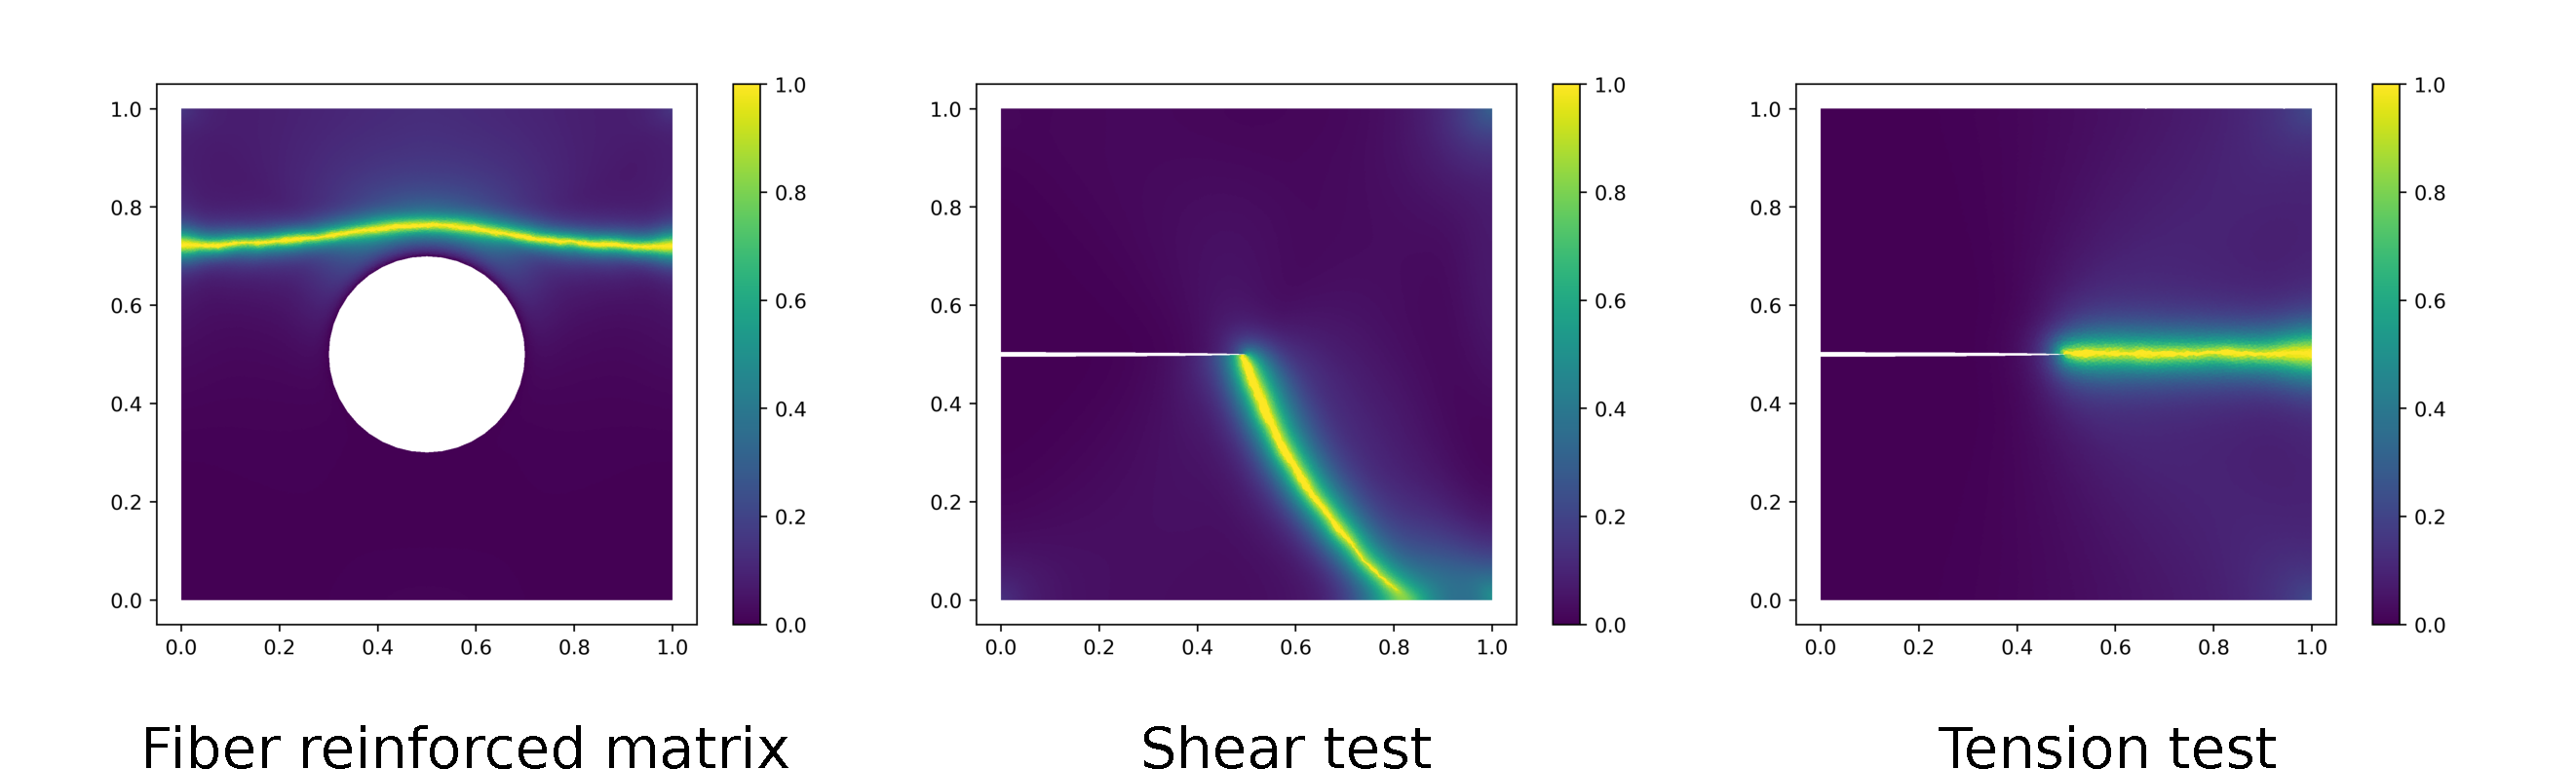
\includegraphics[width=10.cm]{../chapter_003_ef_micromorphic/figures/DamagePattern.pdf}
  \caption{Damage patterns at the end of the unit tests}
  \label{fig:micromorphicdamage:damage_patterns}
\end{figure}

% ![Damage patterns at the end of the unit tests.](img/DamagePattern.pdf){#fig:micromorphicdamage:damage_patterns}

Those tests are performed using the AT2 model and its micromorphic
counterparts using a spectral decomposition of the elastic free energy.
The damage patterns at the end of those tests are reported on Figure
\ref{fig:micromorphicdamage:damage_patterns}.

The \texttt{python} scripts are available in this repository:
https://github.com/thelfer/micromorphic-damage-giens-2022.

Those scripts contain the geometry, material properties and loadings
required to reproduce those tests.

For those tests, the penalisation parameter \(H_{\chi}\) is chosen as:
\[
H_{\chi}= \beta\,\Frac{G_{c}}{l_{0}}
\]

where \(\beta\) is a normalised penalisation parameter \cite{bharali_computational_2021}.

\subsection{Choice of the convergence criterion of the staggered schemes}

In this paper, the staggered schemes are stopped when the damage becomes
stationnary, i.e. when the absolute difference between two estimates of
the damge is below a given threshold \(\varepsilon_{d}\) at each
integration point.

This criterion is not totally satisfying as it does not ensure that a
true minimum of the Lagrangian is found. We carefully checked that this
is the case for each steps of the numerical experiments described in
this section.

\subsection{Discussion}

Those three tests lead to similar conclusions:

% ![Evolution of the force as a function of the imposed displacement for
% the fiber reinforced matrix test for the third scheme with \(\beta=150\)
% and the standard phase-field schemes based on the resolution of the
% variational inegality or based on Miehe' history
% function](img/FiberReinforcedMatrix-force.pdf){#fig:micromorphic_damage:force
% width=75%}

\begin{figure}[H]
  \centering
  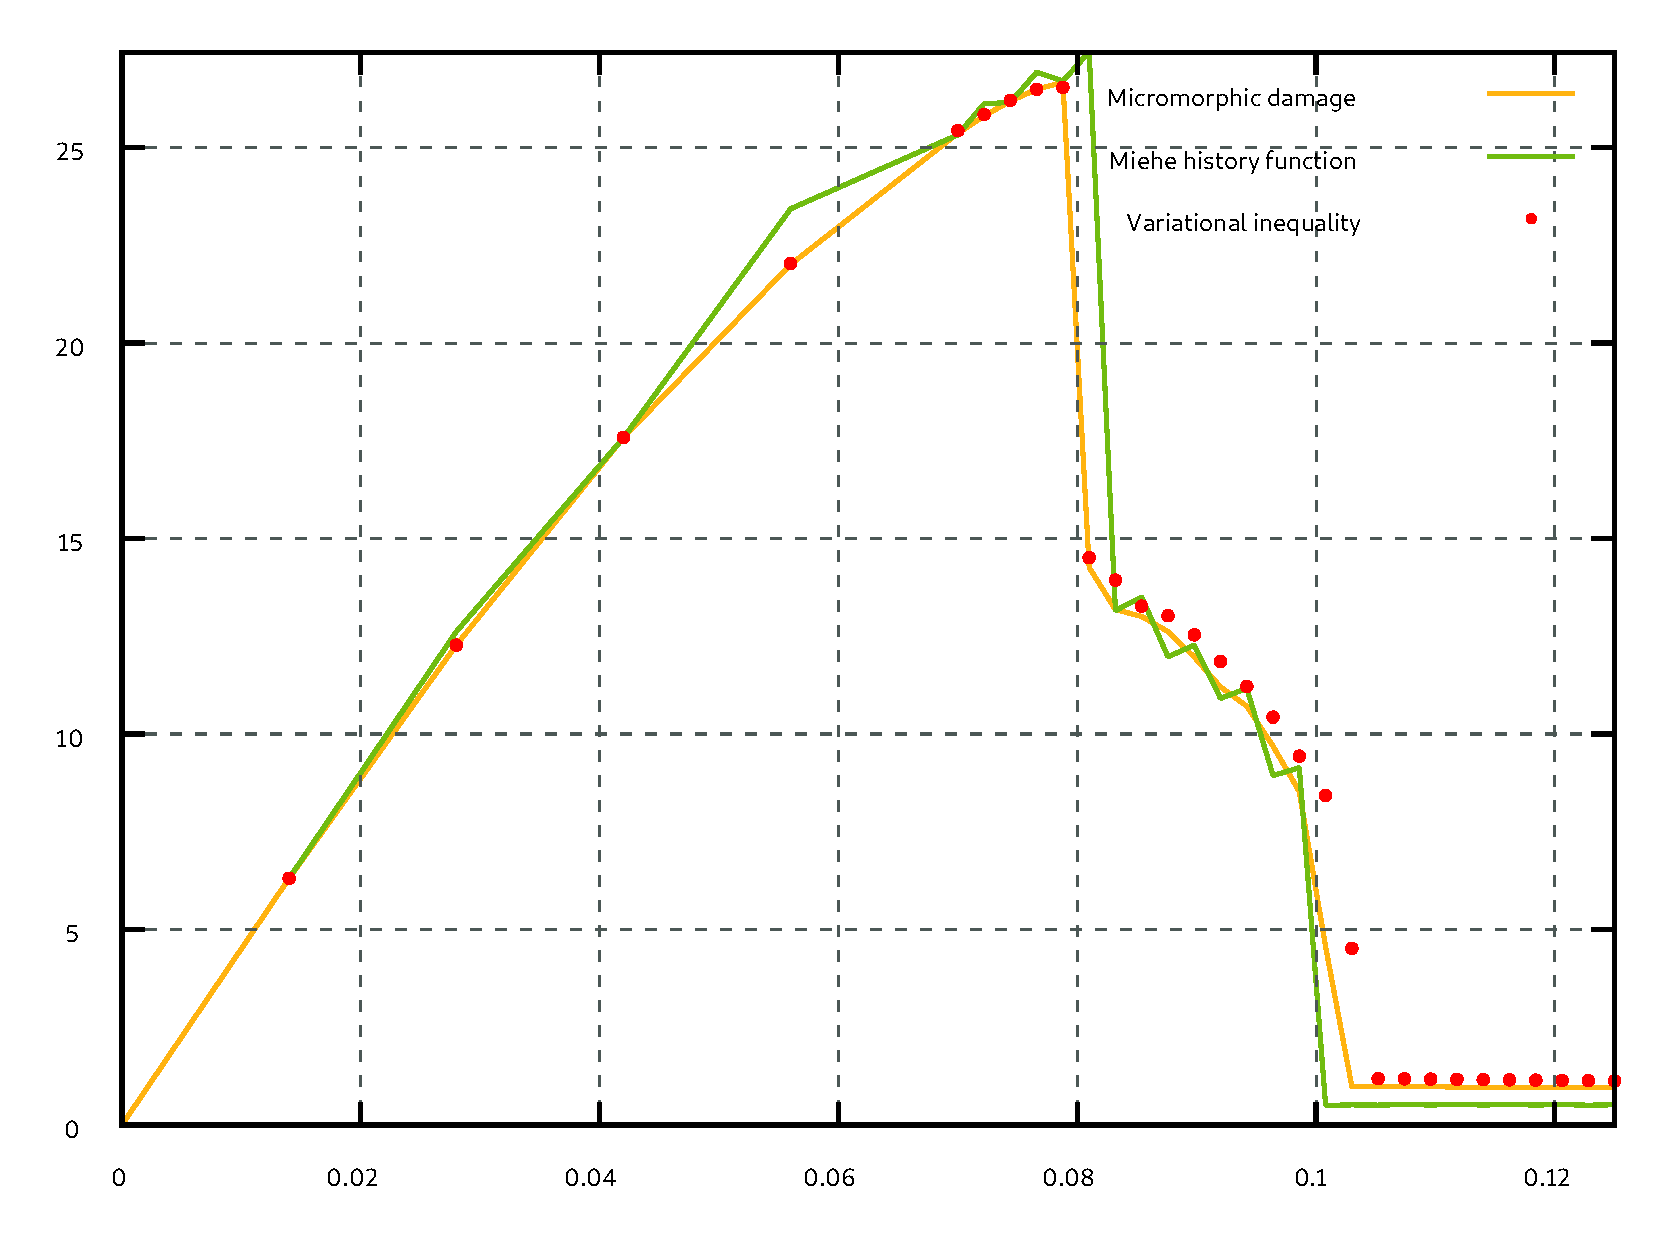
\includegraphics[width=10.cm]{../chapter_003_ef_micromorphic/figures/FiberReinforcedMatrix-force.pdf}
  \caption{Evolution of the force as a function of the imposed displacement for
  the fiber reinforced matrix test for the third scheme with \(\beta=150\)
  and the standard phase-field schemes based on the resolution of the
  variational inegality or based on Miehe' history
  function}
  \label{fig:micromorphic_damage:force}
\end{figure}

% ![Evolution of the force as a function of the imposed displacement for
% \(\beta=50\), \(\beta=100\), \(\beta=150\) for the shear test using the
% third staggered scheme.](img/shear-force.pdf){width=75%
% #fig:micromorphic_damage:beta}

\begin{figure}[H]
  \centering
  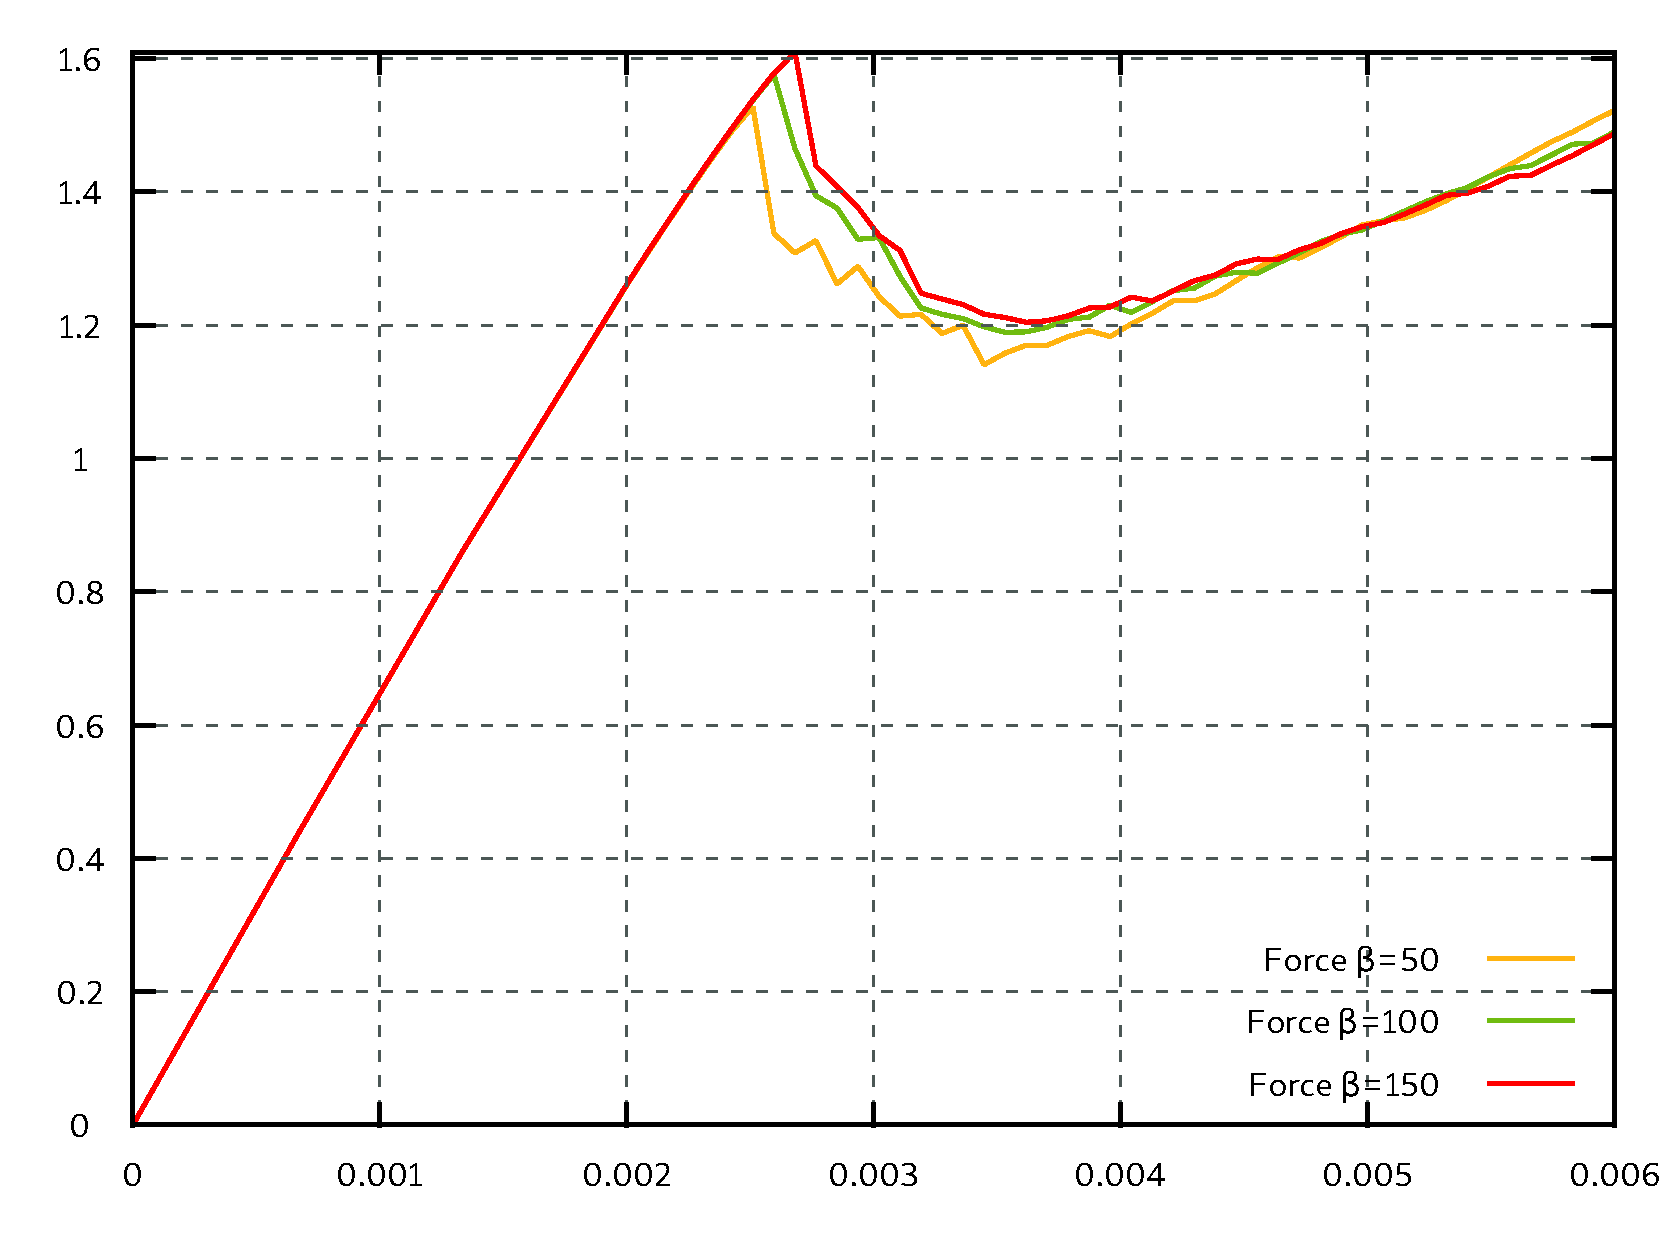
\includegraphics[width=10.cm]{../chapter_003_ef_micromorphic/figures/shear-force.pdf}
  \caption{Evolution of the force as a function of the imposed displacement for
  \(\beta=50\), \(\beta=100\), \(\beta=150\) for the shear test using the
  third staggered scheme}
  \label{fig:micromorphic_damage:beta}
\end{figure}

% ![Evolution of the fracture energy as a function of the imposed
% displacement for \(\beta=50\), \(\beta=100\), \(\beta=150\) for the
% shear test using the third staggered
% scheme.](img/DissipatedEnergies.pdf){width=75%
% #fig:micromorphic_damage:beta2}

\begin{figure}[H]
  \centering
  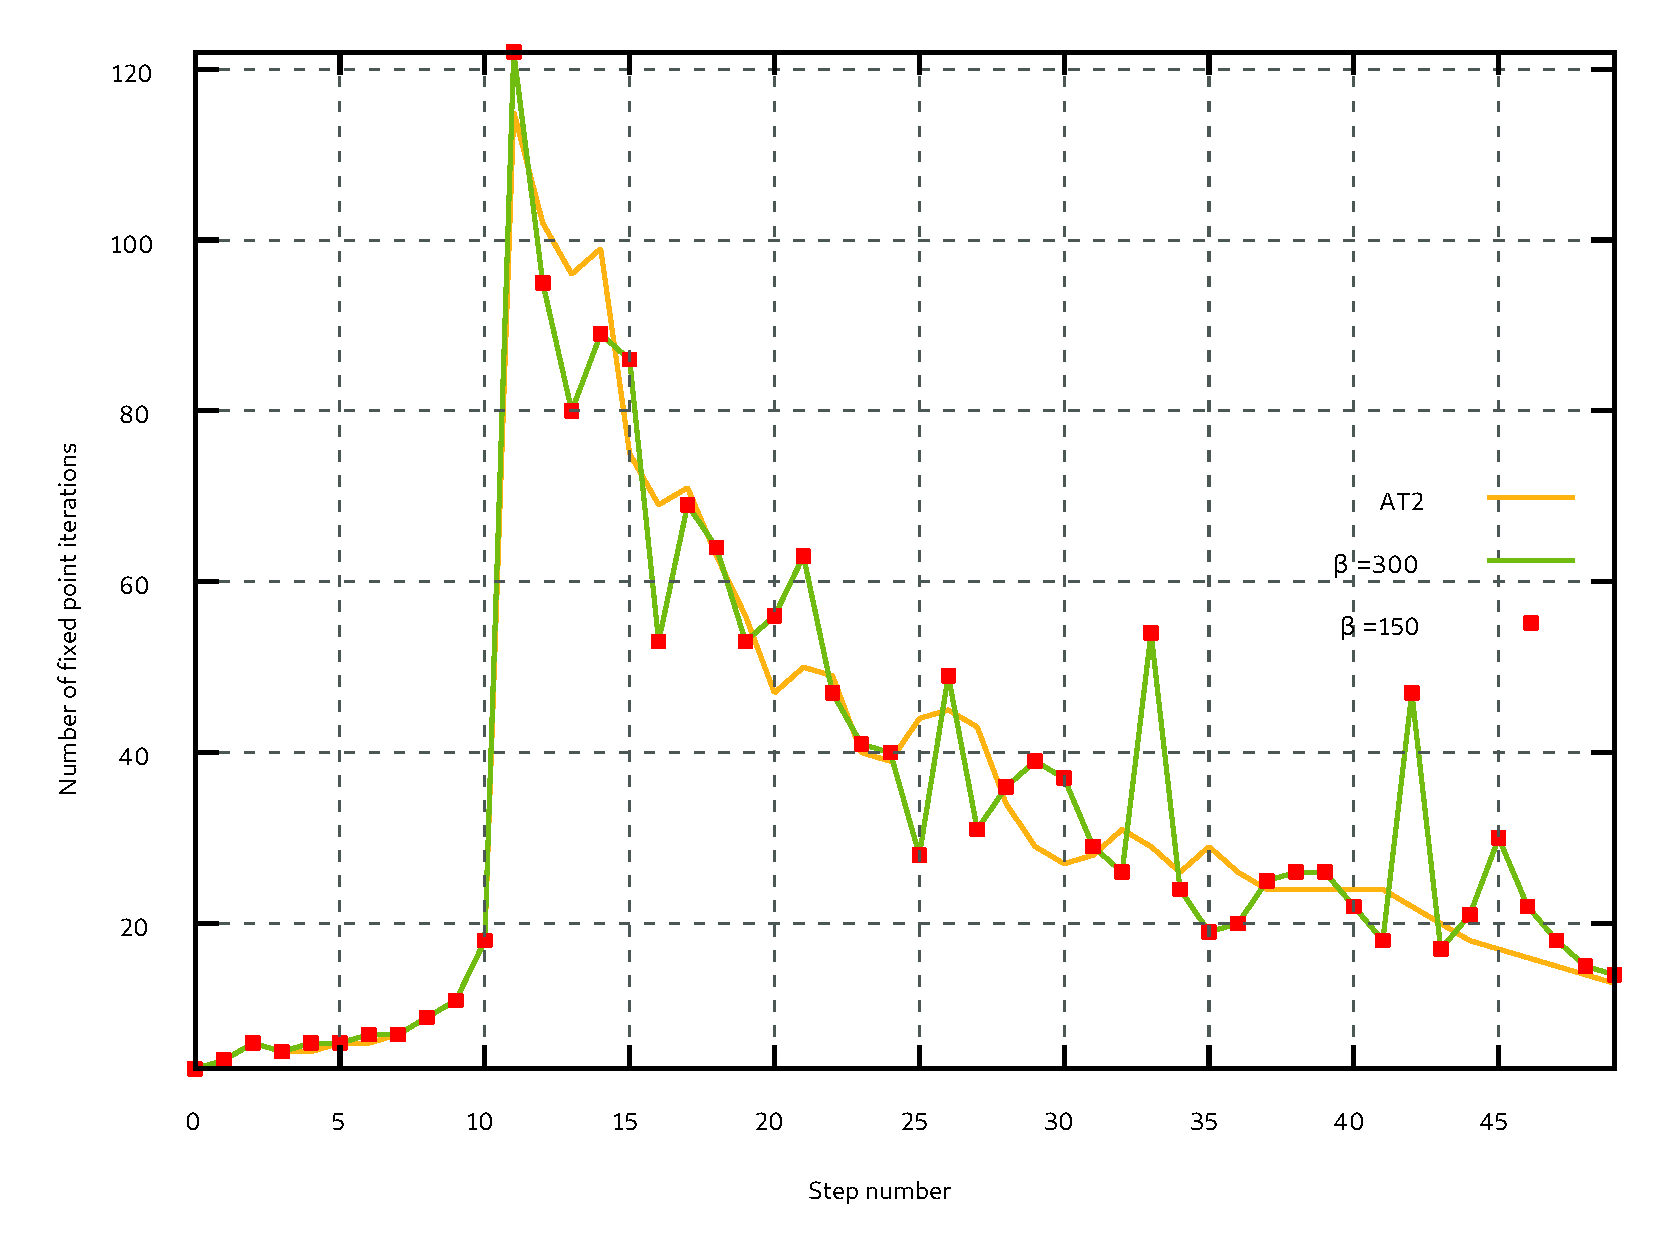
\includegraphics[width=10.cm]{../chapter_003_ef_micromorphic/figures/shear-iterations.pdf}
  \caption{Number of iterations of the fixed point algorithm for the shear test
  as a function of the step number for the standard AT2 model and the
  third scheme for \(\beta=150\) and
  \(\beta=300\)}
  \label{fig:micromorphic_damage:shear:iterations}
\end{figure}

% ![Number of iterations of the fixed point algorithm for the shear test
% as a function of the step number for the standard AT2 model and the
% third scheme for \(\beta=150\) and
% \(\beta=300\).](img/shear-iterations.pdf){width=75%
% #fig:micromorphic_damage:shear:iterations}

\begin{itemize}
  \item The two first schemes converge very slowly (several thousands of fixed
  point iterations) even in the quasi-elastic range. A threshold as
  small as \(10^{-5}\) is required to ensure converged results. Those
  schemes are considered unsuable in pratice.
  \item The third scheme converges much faster. A threshold value of
  \(10^{-3}\) is sufficient to have converged results. The same
  threshold value is used for the standard AT2 model.
  \item As illustrated by Figure \ref{fig:micromorphic_damage:force}, the
  force-displacement curve of the third scheme is very similar to the
  standard AT2 model.
  \item As illustrated by Figure \ref{fig:micromorphic_damage:beta}, the
  penalisation factor plays a major role on the overall
  force-displacement curve. Our experiments shows that a value of
  \(150\) leads to results undistinguishable with the one of the AT2
  model for all the tests. However, an higher value of \(300\) is
  required to reproduce closely the evolution of the fracture energy.
  \item The number of iteration of the fixed point algorithm is roughly
  similar between the standard AT2 model and the third scheme, altough a
  bit higher in general, as depicted on Figure
  \ref{fig:micromorphic_damage:shear:iterations}.
\end{itemize}

\subsection{Numerical Experiments}
\label{sec:micromorphicdamage:numerical_experiments}

In this section, the \texttt{MFEM/MGIS} solver is used.

\subsubsection{Shear driven fracture}

Alessi et al. proposed a model to describe deviatoric driven fracture
using the following choice of the elastic free energy
\cite{alessi_phase-field_2020}:
\[
\freeenergyel\paren{\tepsilon, d}=
% \Frac{K}{2}\,\paren{\trace{\tepsilon}}^{2}+
% \mu\,g\paren{d}\,\tenseur{s}^{\varepsilon}\,\colon\,\tenseur{s}^{\varepsilon}
\]
where \(K\) is the bulk modulus, \(\tenseur{s}^{\varepsilon}\) is the
deviatoric part of the elastic strain. The degradation function
\(g\paren{d}\) and the other terms of the Lagrangian are the same as in
the AT2 model.

As stated by Alessi et al., this model lead to quasi-incompressible
behaviour in highly damaged zones and proposed a simple tensile test on
a bar which demonstrated that standard Lagrange elements are not able to
properly describe the damage localisation band and the dissipated energy
by the crack propagation. Alessi et al. then showed that various
classical approaches (selective reduced integration and mixed
displacement/pressure formulation) can overcome this issue.

This test is adapted in this section to demonstrate that the
micromorphic approaches can be used with higher order finite elements.
The same order of approximation will be used to solve the mechanical and
the micromorphic problems.

\subsubsection{Geometry, loadings and meshes}

The specimen is a \(2D\) plate of width \(w\) and height \(h\) treated
under the plane strain hypothesis. The axial displacement of the lower
boundary is set to zero, while the axial displacement of the upper
boundary is imposed. The point at the lower left corner is fixed in the
lateral direction to avoid rigid body motion.

% : Geometry and material parameters for the shear driven fracture test.
% {#tbl:micromorphicdamage:shear_driven_fracture_test_parameters}

% +----------------------------------+-----------------------------+
% | Plate width \(w\)                | \(10^{-3}\, m\)             |
% +----------------------------------+-----------------------------+
% | Plate height \(h\)               | \(2\,\cdot\,10^{-3}\, m\)   |
% +----------------------------------+-----------------------------+
% | Young's modulus \(E\)            | \(210\,\cdot\,10^{9}\, Pa\) |
% +----------------------------------+-----------------------------+
% | Poisson's ratio \(\nu\)          | \(0.3\)                     |
% +----------------------------------+-----------------------------+
% | Fracture energy \(G_{c}\)        | \(2.7\,J.m^{-2}\)           |
% +----------------------------------+-----------------------------+
% | Characteristic length  \(l_{0}\) | \(2.5\,\cdot\,10^{-5}\,m\)  |
% +----------------------------------+-----------------------------+
% | Penalisation factor \(\beta\)    | \(300\)                     |
% +----------------------------------+-----------------------------+

\begin{table}[H]
    \centering
    \begin{tabular}{||c c||} 
        \hline
        Resolution Method & Memory footprint
        \\
        [0.5ex] 
        \hline\hline
        Plate width \(w\)                & \(10^{-3}\, m\)             
        \\ \hline
        Plate height \(h\)               & \(2\,\cdot\,10^{-3}\, m\)   
        \\ \hline
        Young's modulus \(E\)            & \(210\,\cdot\,10^{9}\, Pa\) 
        \\ \hline
        Poisson's ratio \(\nu\)          & \(0.3\)                     
        \\ \hline
        Fracture energy \(G_{c}\)        & \(2.7\,J.m^{-2}\)           
        \\ \hline
        Characteristic length  \(l_{0}\) & \(2.5\,\cdot\,10^{-5}\,m\)  
        \\ \hline
        Penalisation factor \(\beta\)    & \(300\)                     
        \\ \hline
    \end{tabular}
    \caption{Geometry and material parameters for the shear driven fracture test}
    \label{tbl:micromorphicdamage:shear_driven_fracture_test_parameters}
\end{table}


The geometry and the material parameters used for this test are
summarized in Table
\ref{tbl:micromorphicdamage:shear_driven_fracture_test_parameters}. In order
to localize the damage, the fracture energy is assumed uniform in the
plate except in a small square of size \(5\,\cdot\,10^{-2}\,\cdot\,w\)
located at the center of the plate where the fracture energy value is
\(G_{c}\,\cdot\,\paren{1-10^{-2}}\).

: Number of elements for the shear driven fracture test. A very fine
mesh is used for low order finite elements (\(1\) and \(2\)) with
several dozen elements inside the damage band (See Figure
\ref{fig:micromorphicdamage:shear_driven_fracture_test_order1}). A coarser
mesh is used for higher order elements (\(4\) and \(6\)) with \(4\) to
\(6\) elements inside the damage band.

% {#tbl:micromorphicdamage:shear_driven_fracture_test_elements}

% +---------+-----------------------+
% | Order 1 | \(102\,272\) elements |
% +---------+-----------------------+
% | Order 2 | \(409\,088\) elements |
% +---------+-----------------------+
% | Order 4 | \(25\,568\) elements  |
% +---------+-----------------------+
% | Order 6 | \(25\,568\) elements  |
% +---------+-----------------------+

\begin{table}[H]
    \centering
    \begin{tabular}{||c c||} 
        \hline
        Resolution Method & Memory footprint
        \\
        [0.5ex] 
        \hline\hline
        Order 1 & \(102\,272\) elements
        \\ \hline
        Order 2 & \(409\,088\) elements
        \\ \hline
        Order 4 & \(25\,568\) elements 
        \\ \hline
        Order 6 & \(25\,568\) elements 
        \\ \hline
    \end{tabular}
    \caption{Geometry and material parameters for the shear driven fracture test}
    \label{tbl:micromorphicdamage:shear_driven_fracture_test_elements}
\end{table}

The plate is discretized with triangle elements. The number of elements
used as a function of the finite element order is given in Table
\ref{tbl:micromorphicdamage:shear_driven_fracture_test_elements}. In
practice, this number of elements have little influence on the results
and the conclusions drawn in the next paragraph.

\subsection{Results}

\begin{figure}[H]
  \centering
  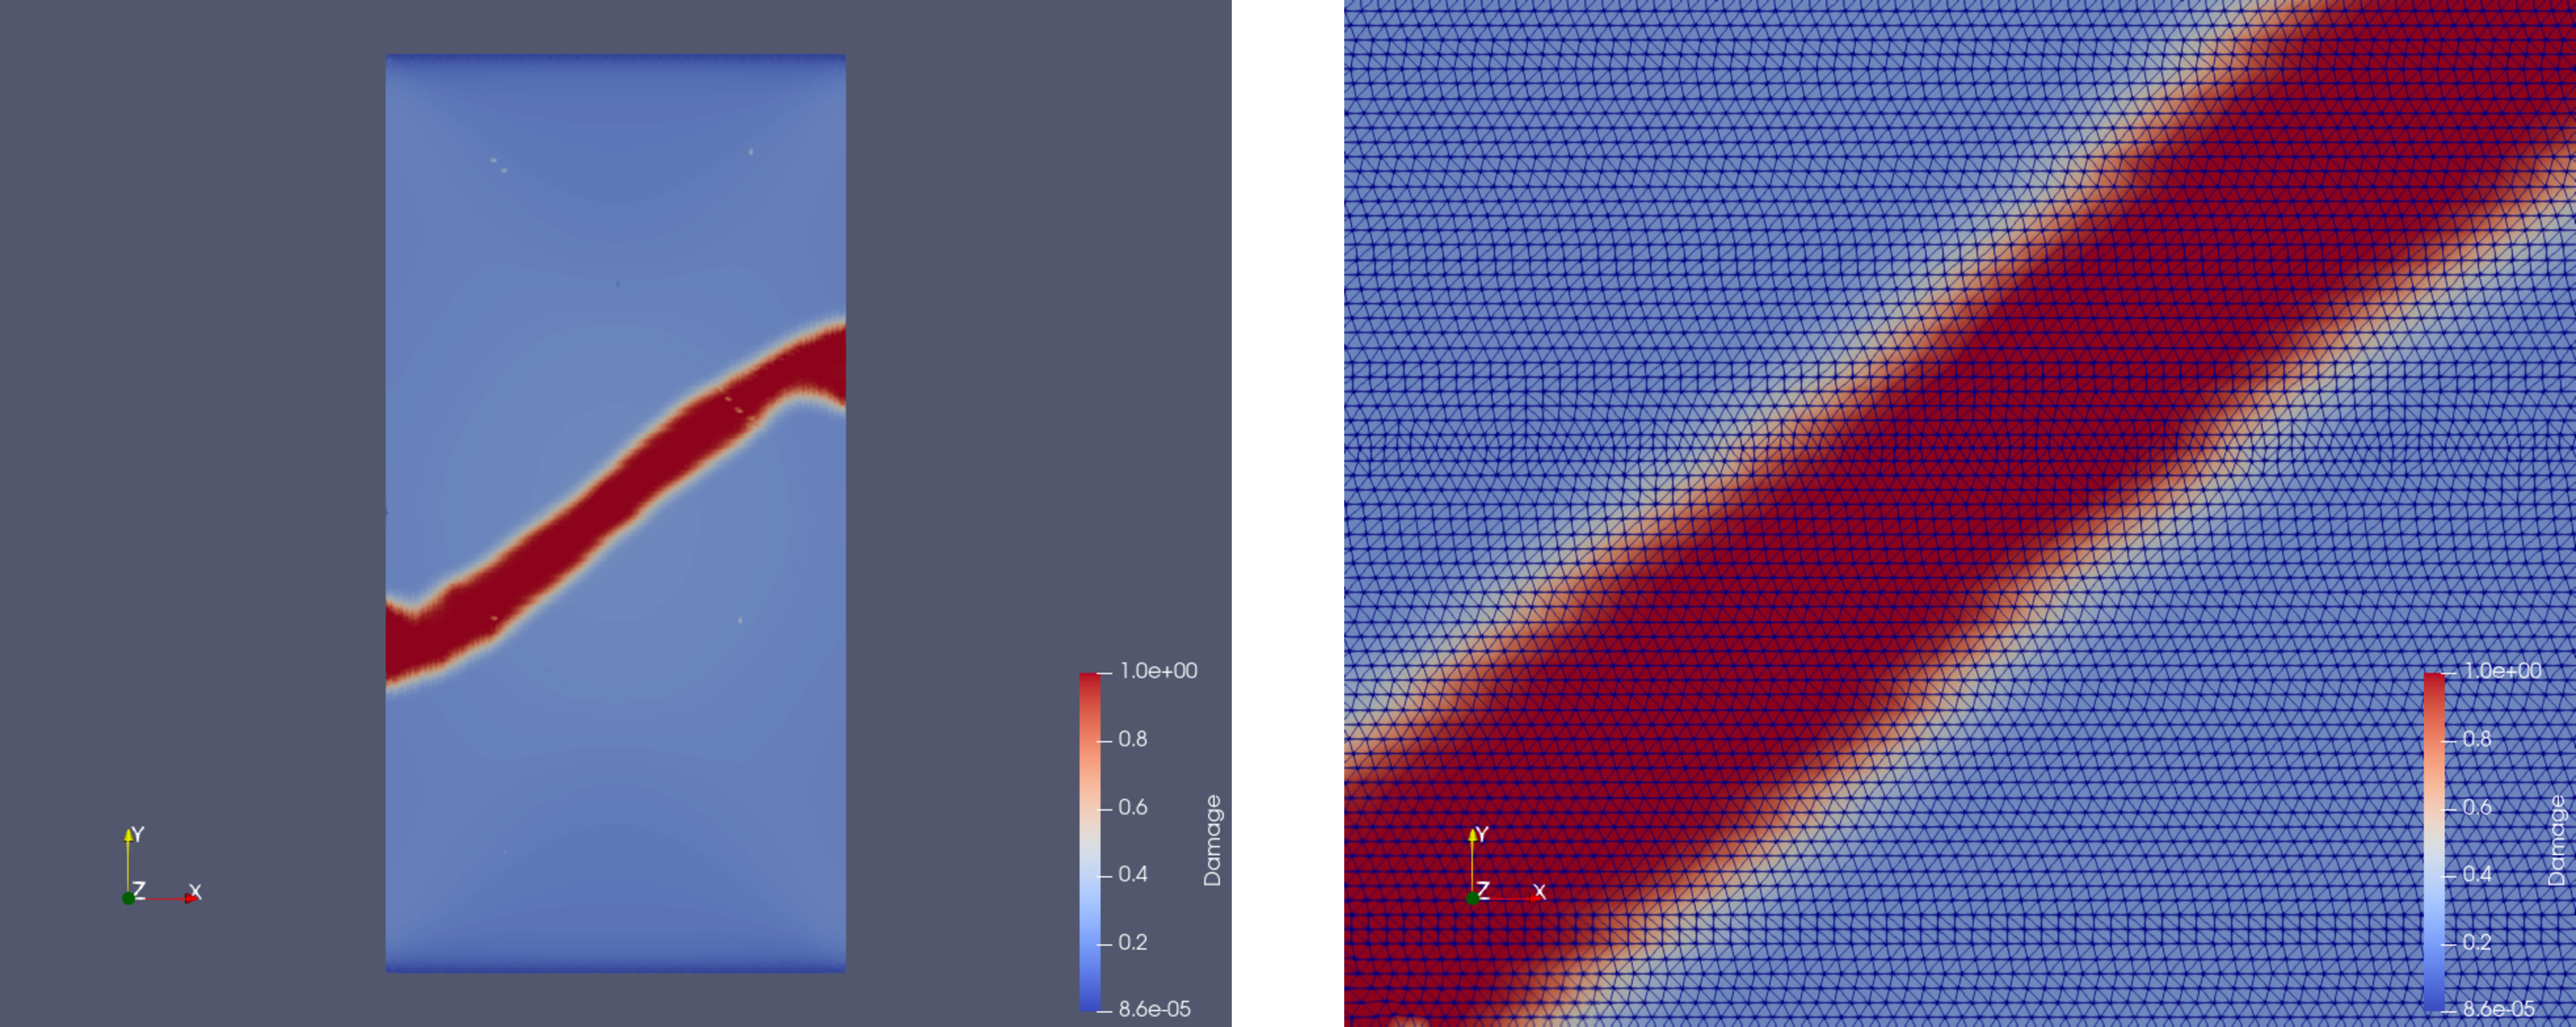
\includegraphics[width=10.cm]{../chapter_003_ef_micromorphic/figures/shear-driven-fracture-damage-results-order-1.pdf}
  \caption{Spurious damage map obtained with linear elements (left). Zoom on the shear fracture (right)}
  \label{fig:micromorphicdamage:shear_driven_fracture_test_order1}
\end{figure}

% ![Spurious damage map obtained with linear elements (left). Zoom on the shear fracture (right)](img/shear-driven-fracture-damage-results-order-1.pdf){#fig:micromorphicdamage:shear_driven_fracture_test_order1 width=75%}

Figure \ref{fig:micromorphicdamage:shear_driven_fracture_test_order1}
describes the damage map pattern after the propagation of the crack. As
described by Alessi et al., volumetric locking leads to a spurious
damage localisation band with excessive thickness, i.e. a thickness
largely greater than the characteristic length \(l_{0}\). A very fine
mesh is used to demonstrate that the issue is not solved by mesh
refinement.

% ![Damage map for higher order elements. Quadradic elements (left), fourth order elements (center), sixth order elements (right). The quadratic mesh is too fine to be shown without hiding the results.](img/shear-driven-fracture-damage-results-higher-orders.pdf){#fig:micromorphicdamage:shear_driven_fracture_test_higher_order width=100%}

\begin{figure}[H]
  \centering
  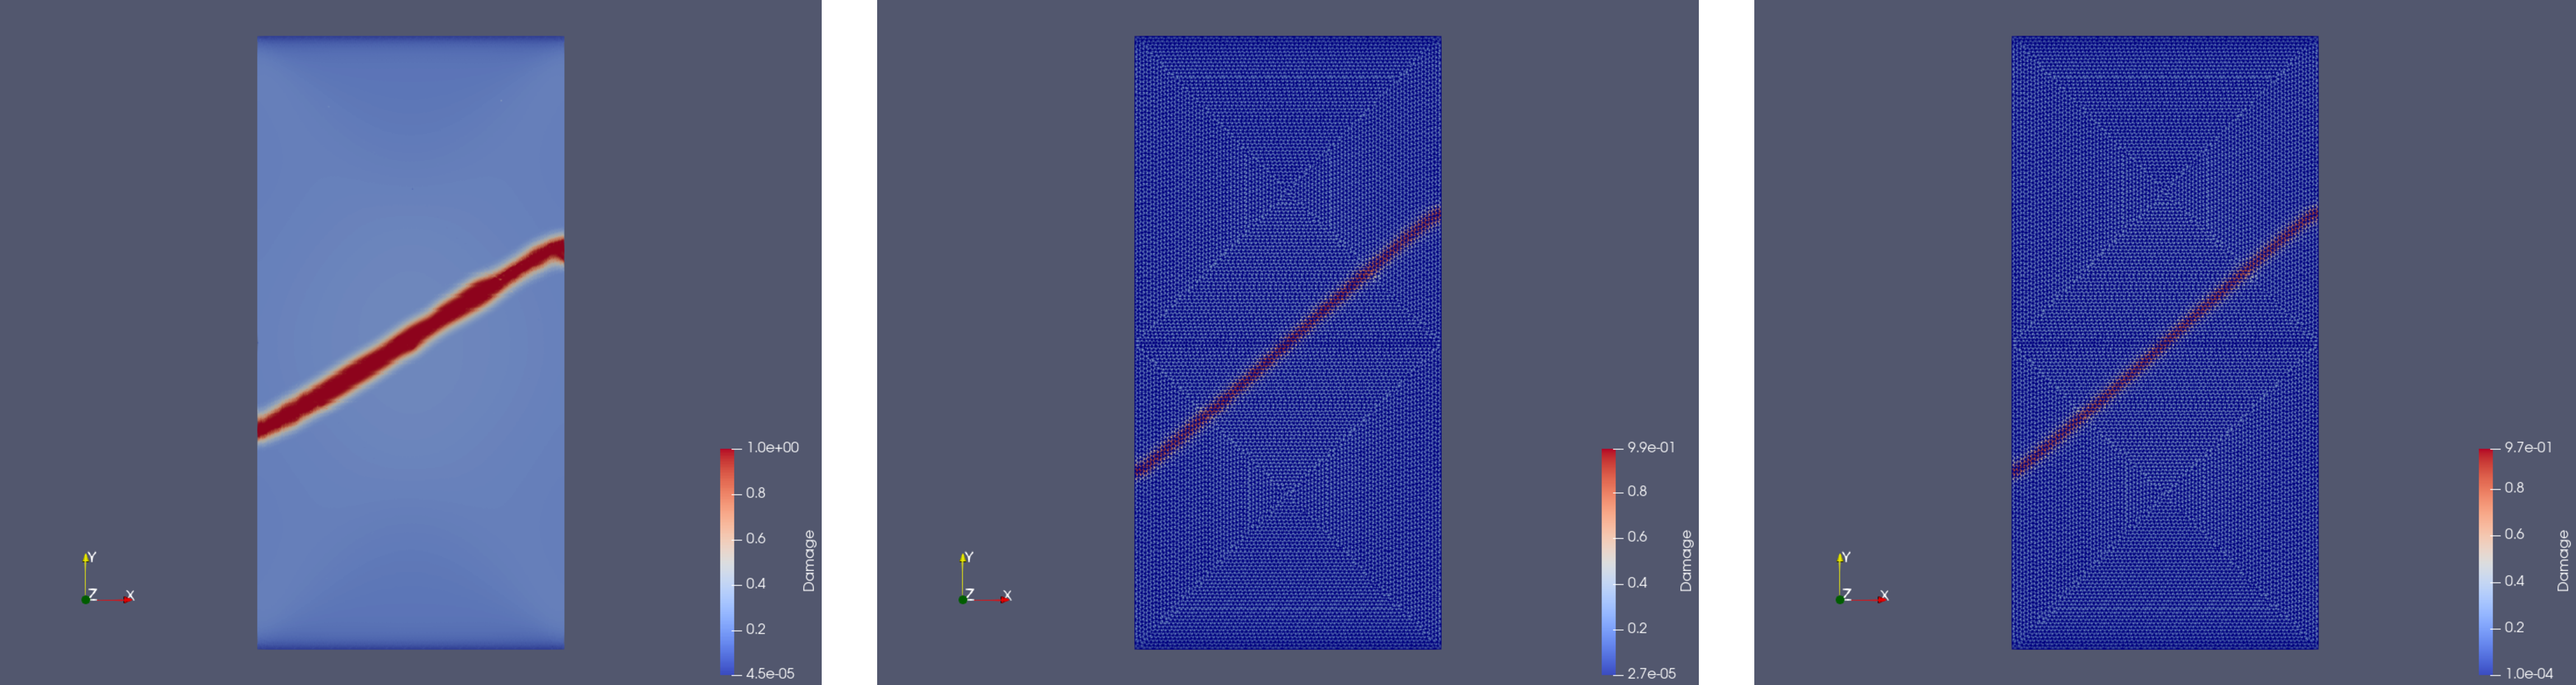
\includegraphics[width=10.cm]{../chapter_003_ef_micromorphic/figures/shear-driven-fracture-damage-results-higher-orders.pdf}
  \caption{Damage map for higher order elements. Quadradic elements (left), fourth order elements (center), sixth order elements (right). The quadratic mesh is too fine to be shown without hiding the results}
  \label{fig:micromorphicdamage:shear_driven_fracture_test_higher_order}
\end{figure}

Figure \ref{fig:micromorphicdamage:shear_driven_fracture_test_higher_order}
show the results obtained with higher order elements. While the
simulation with quadratic elements still exhibit a spurious damage
localisation band, similar to the one observed with linear elements in
Figure \ref{fig:micromorphicdamage:shear_driven_fracture_test_order1}, higher
order elements lead to satisfying results, i.e. higher order elements
alleviate issues related to volumetric locking.

% ![Traction curve](img/shear-driven-fracture-damage-results-force.pdf){#fig:micromorphicdamage:traction_curve width=75%}

\begin{figure}[H]
  \centering
  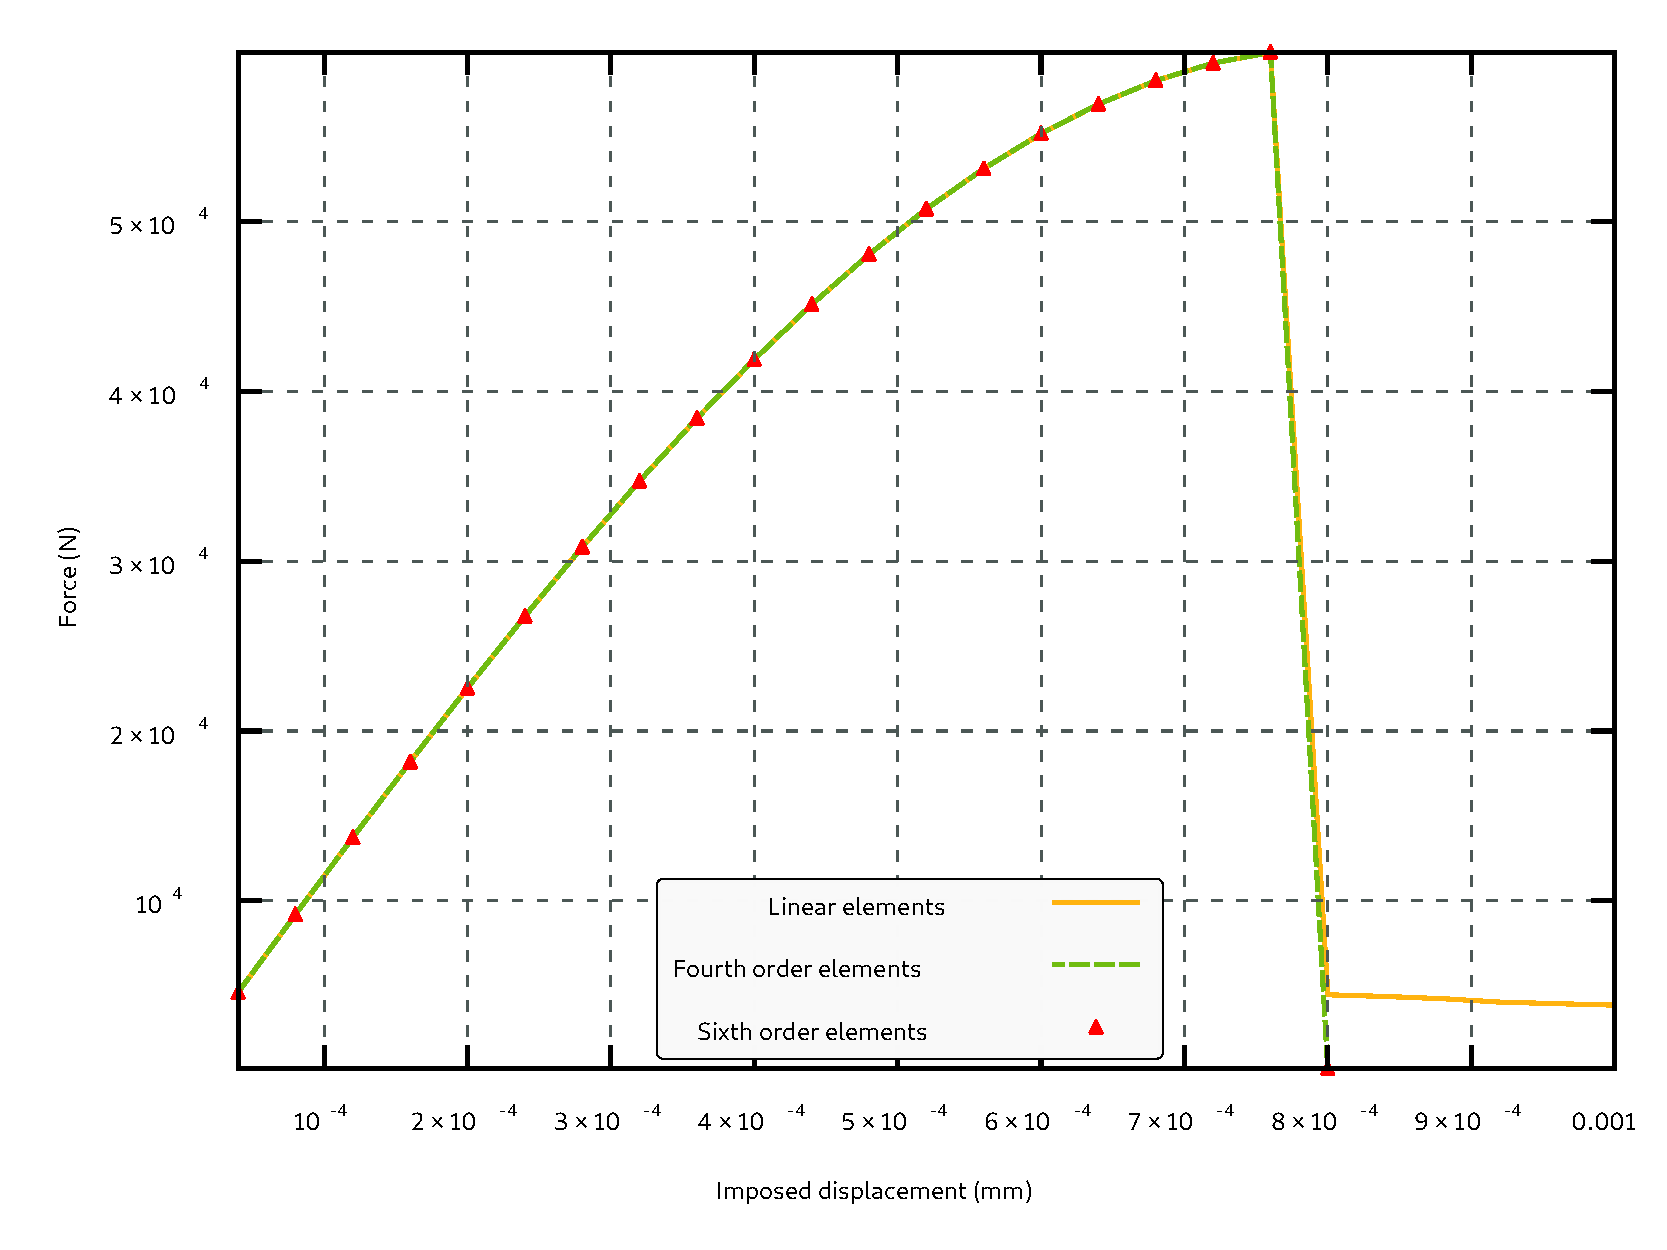
\includegraphics[width=10.cm]{../chapter_003_ef_micromorphic/figures/shear-driven-fracture-damage-results-force.pdf}
  \caption{Traction curve}
  \label{fig:micromorphicdamage:traction_curve}
\end{figure}

Figure \ref{fig:micromorphicdamage:traction_curve} presents the
force/displacement curves as a function of the finite element order.
Quadratic results, which are intermediate between linear and quadratic
results, are not reproduced for the sake of clarity. The following
observations can be made:

\begin{itemize}
  \item All order of approximations give similar results up to the crack
  progation.
  \item The traction curve given by linear elements exhibits a residual
  stifness and a spurious dissipation after the crack propagation.
  \item Fourth order and sixth order give undistinguishable results. In both
  cases, the force drops to zero after the crack propagation.
\end{itemize}

\subsection{Industrial test case: nuclear fuel pellet fragmentation}

In this section, the fragmentation of a nuclear fuel pellet during the
reactor start-up. 

\paragraph{Geometry, material and loadings}

% : Geometry, material parameters and loading parameters for the fuel pellet fragementation test.
% {#tbl:micromorphicdamage:fuel_pellet_fragmentation_test_parameters}

% +--------------------------------------------------------------+-----------------------------+
% | Pellet radius \(r_{p}\)                                      | \(4.085\,\cdot\,10^{-3}\)   |
% +--------------------------------------------------------------+-----------------------------+
% | Pellet height \(h_{p}\)                                      | \(6.7\,\cdot\,10^{-3}\)     |
% +--------------------------------------------------------------+-----------------------------+
% | Dishing radius \(r_{d}\)                                     | \(3.05\,\cdot\,10^{-3}\)    |
% +--------------------------------------------------------------+-----------------------------+
% | Dishing height \(h_{d}\)                                     | \(3.2\,\cdot\,10^{-4}\)     |
% +--------------------------------------------------------------+-----------------------------+
% | Young's modulus \(E\)                                        | \(150\,\cdot\,10^{9}\, Pa\) |
% +--------------------------------------------------------------+-----------------------------+
% | Poisson's ratio \(\nu\)                                      | \(0.3\)                     |
% +--------------------------------------------------------------+-----------------------------+
% | Linear mean thermal expansion coefficient \(\alpha\)         | \(1\,\cdot\,10^{-5}\)       |
% +--------------------------------------------------------------+-----------------------------+
% | Thermal expansion reference temperature \(T_{\mathrm{ref}}\) | \(1\,\cdot\,10^{-5}\)       |
% +--------------------------------------------------------------+-----------------------------+
% | Fracture energy \(G_{c}\)                                    | \(xxx\,J.m^{-2}\)           |
% +--------------------------------------------------------------+-----------------------------+
% | Characteristic length  \(l_{0}\)                             | \(xxx\,\cdot\,10^{-xx}\,m\) |
% +--------------------------------------------------------------+-----------------------------+
% | Penalisation factor \(\beta\)                                | \(300\)                     |
% +--------------------------------------------------------------+-----------------------------+
% | Core temperature\(T_{c}\)                                    | \(1500\,K\)                 |
% +--------------------------------------------------------------+-----------------------------+
% | Outer surface temperature \(T_{o}\)                          | \(600\,K\)                  |
% +--------------------------------------------------------------+-----------------------------+

\begin{table}[H]
    \centering
    \begin{tabular}{||c c||} 
        \hline
        Resolution Method & Memory footprint
        \\
        [0.5ex] 
        \hline\hline
        Pellet radius \(r_{p}\)                                      & \(4.085\,\cdot\,10^{-3}\)   
        \\ \hline
        Pellet height \(h_{p}\)                                      & \(6.7\,\cdot\,10^{-3}\)     
        \\ \hline
        Dishing radius \(r_{d}\)                                     & \(3.05\,\cdot\,10^{-3}\)    
        \\ \hline
        Dishing height \(h_{d}\)                                     & \(3.2\,\cdot\,10^{-4}\)     
        \\ \hline
        Young's modulus \(E\)                                        & \(150\,\cdot\,10^{9}\, Pa\) 
        \\ \hline
        Poisson's ratio \(\nu\)                                      & \(0.3\)                     
        \\ \hline
        Linear mean thermal expansion coefficient \(\alpha\)         & \(1\,\cdot\,10^{-5}\)       
        \\ \hline
        Thermal expansion reference temperature \(T_{\mathrm{ref}}\) & \(1\,\cdot\,10^{-5}\)       
        \\ \hline
        Fracture energy \(G_{c}\)                                    & \(xxx\,J.m^{-2}\)           
        \\ \hline
        Characteristic length  \(l_{0}\)                             & \(xxx\,\cdot\,10^{-xx}\,m\) 
        \\ \hline
        Penalisation factor \(\beta\)                                & \(300\)                     
        \\ \hline
        Core temperature\(T_{c}\)                                    & \(1500\,K\)                 
        \\ \hline
        Outer surface temperature \(T_{o}\)                          & \(600\,K\)            
        \\ \hline
    \end{tabular}
    \caption{Geometry, material parameters and loading parameters for the fuel pellet fragementation test}
    \label{tbl:micromorphicdamage:fuel_pellet_fragmentation_test_parameters}
\end{table}

\subsection{Thermal expansion}

The strain \(\tepsilonth\) associated with the thermal expansion is
computed as follows:
\[
\tepsilonth\paren{T}=\alpha\,\paren{T-T_{\mathrm{ref}}}\,\tenseur{I}
\]
where:

- \(T\) is the temperature.
- \(T_{\mathrm{ref}}\) is a reference temperature.
- \(\alpha\) is the mean linear thermal expansion coefficient.

\subsection{Modification of the free energy}

To take the thermal expansion into account, the free energy
\(\freeenergyel\paren{\tepsilon, d}\) is modified as follows:

\begin{equation}
  \label{eq:micromorphicdamage:freeenergygel_2}
  \freeenergyel\paren{\tepsilon, T, d} = 
  g\paren{d}\,\freeenergyel_{0}\paren{\tepsilon-\tepsilonth} =
  \Frac{g\paren{d}}{2}\,\paren{\tepsilon-\tepsilonth}\,\colon\,\tenseurq{D}\,\colon\,\paren{\tepsilon-\tepsilonth}
\end{equation}

% \[
% \freeenergyel\paren{\tepsilon, T, d} = 
% g\paren{d}\,\freeenergyel_{0}\paren{\tepsilon-\tepsilonth} =
% \Frac{g\paren{d}}{2}\,\paren{\tepsilon-\tepsilonth}\,\colon\,\tenseurq{D}\,\colon\,\paren{\tepsilon-\tepsilonth}
% \]{#eq:micromorphicdamage:freeenergygel}

\subsection{Temperature profile}

Under the approximation of a constant thermal conductivity, the
temperature profile in a PWR fuel pellet is axisymmetric and parabolic:
\[
T\paren{r, t}=\Delta\,T\paren{t}\,\paren{1-r^{2}}+T_{\mathrm{o}}
\]
where:

\begin{itemize}
  \item \(t\) is a loading parameter in the range \([0:1]\).
  \item \(T_{\mathrm{o}}\) is the temperature at the outer boundary of the
    fuel pellet.
  \item The temperature increase \(\Delta\,T\paren{t}\) is chosen as a linear
    function of the loading parameter as follows:
    \[
    \Delta\,T\paren{t} = \paren{T_{\mathrm{c}}-T_{\mathrm{o}}}\, t
    \]
\end{itemize}

\subsection{Results}

\(33\,230\,848\) triangles, \(132'923'392\) nodes, \(4.10^8\) degrees of freedom for the mechanical problem.

% ![Crack pattern](img/FuelPelletCracking-results.pdf){width=75%}

\begin{figure}[H]
  \centering
  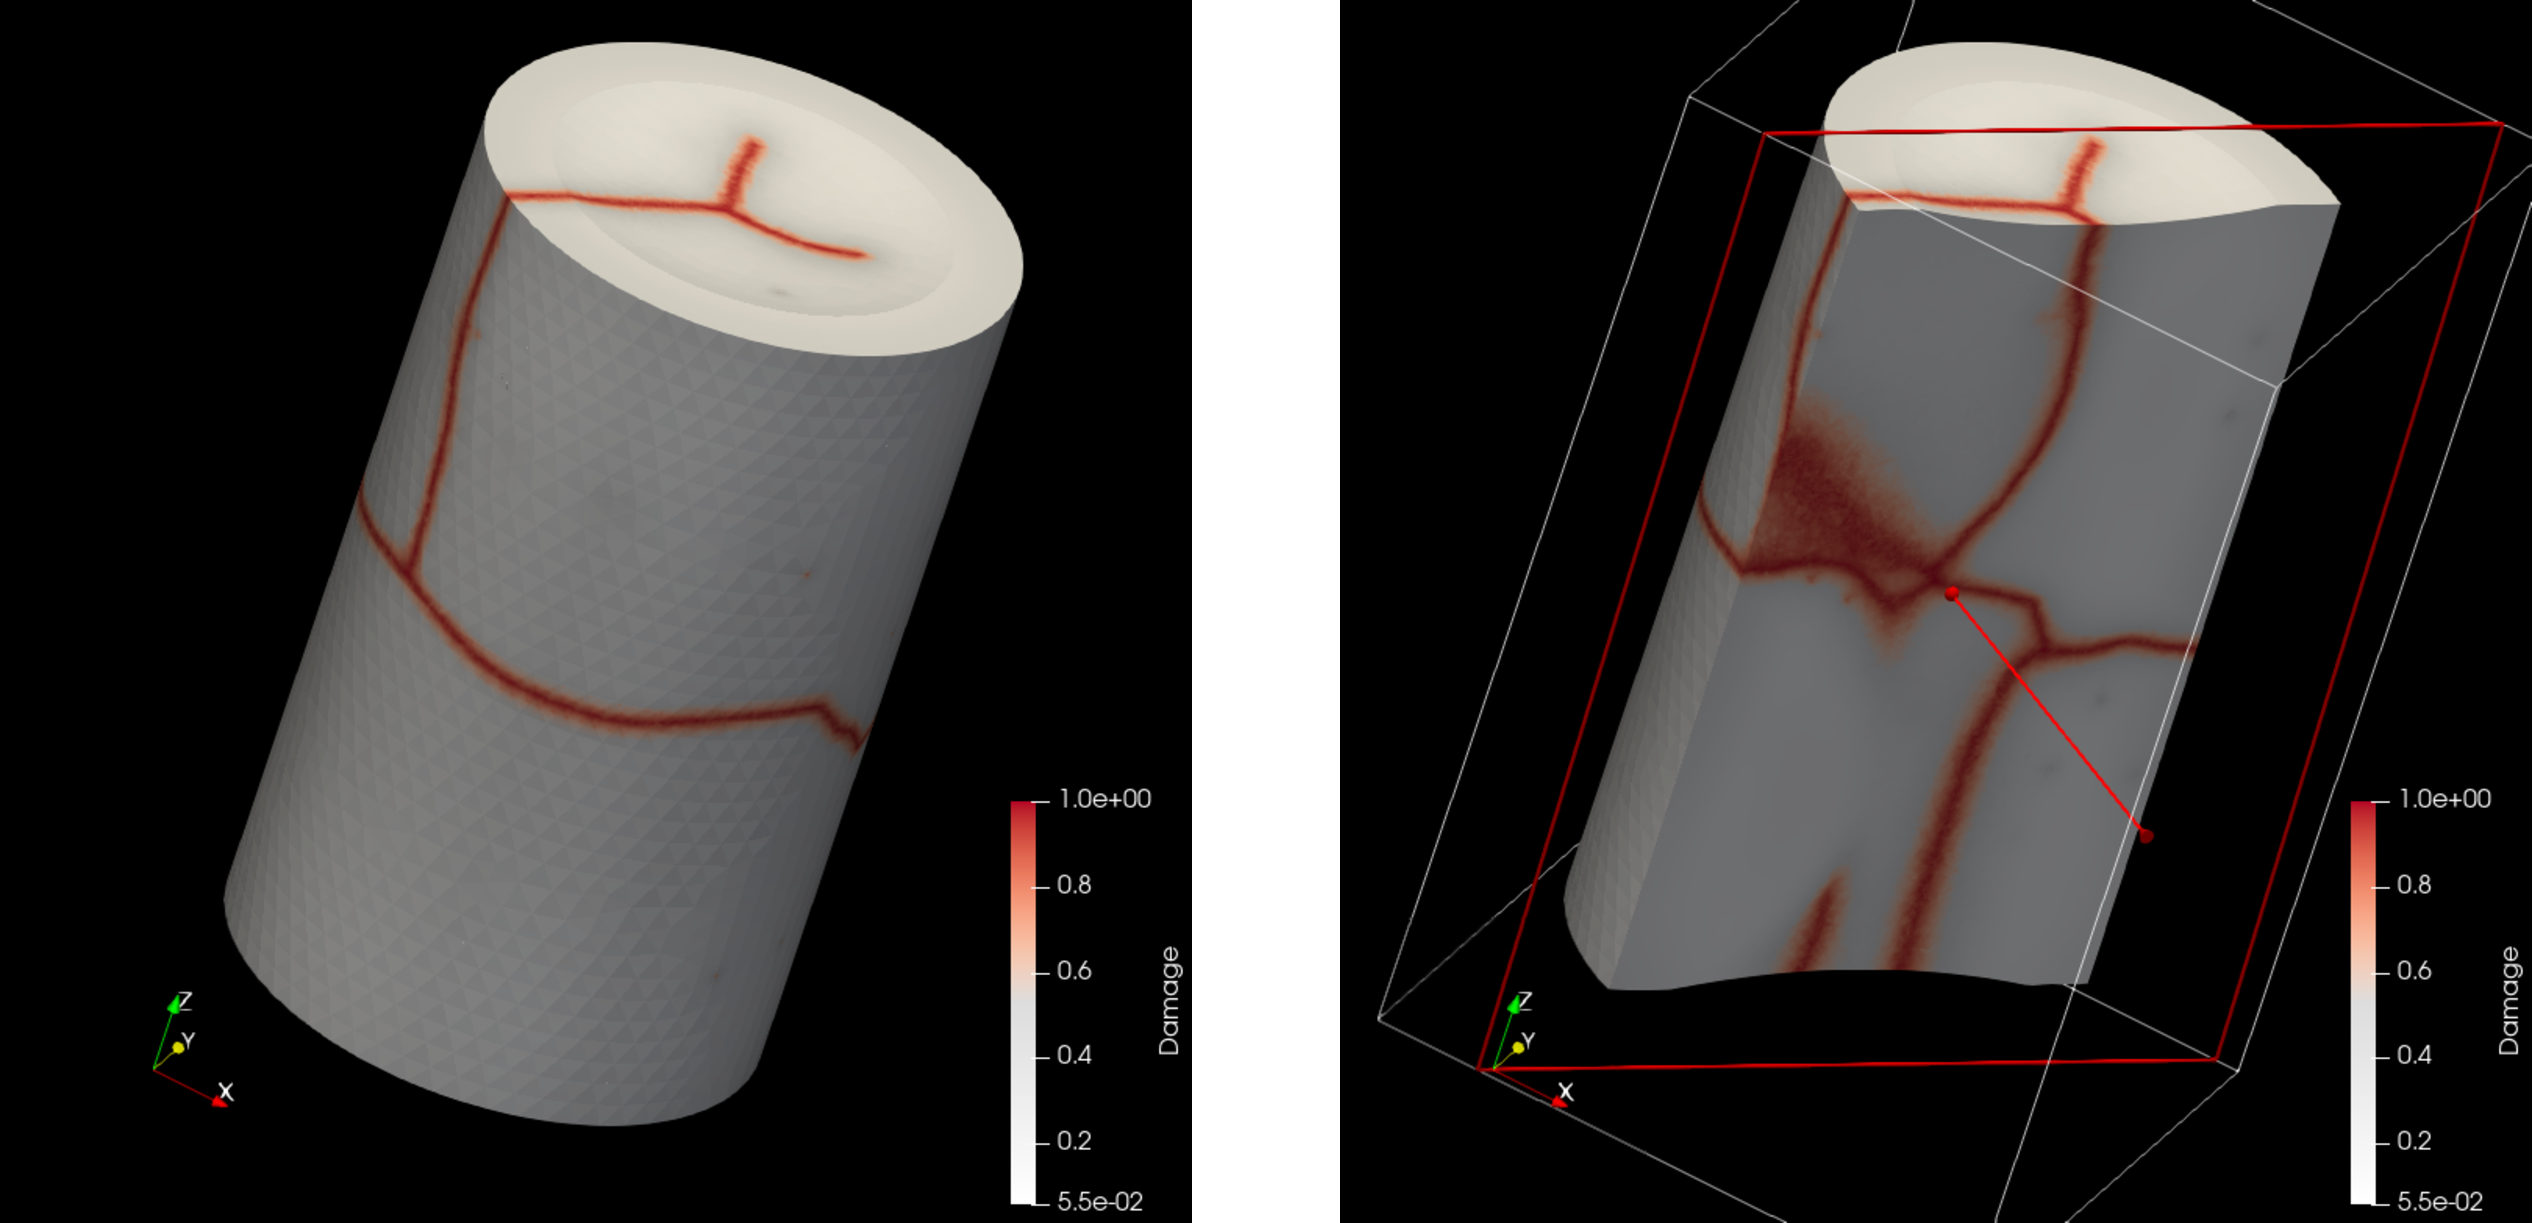
\includegraphics[width=10.cm]{../chapter_003_ef_micromorphic/figures/FuelPelletCracking-results.pdf}
  \caption{Crack pattern}
\end{figure}

\subsection{Conclusions and perspectives}

This work has investigated the use of micromorphic behaviours for the
description of quasi-brittle materials and has shown that those
micromorphic behaviours can be considered as varitionally consistent
approximations of standard phase-field models.

Three alternate minimisation schemes, which are straightforward to
implement in standard FEM or FFT solvers, have been proposed, and their numerical performance has been investigated intensively using representative tests. 

Convergence of those schemes is guaranteed but requires a large number
of fixed-point iterations. Regarding this observation, the third
scheme appears to be more efficient.

The proposed approach can be extended to more complex damage behaviours
and ductile failure.

However, as a future work, acceleration schemes could also be
investigated to reduce the number of fixed-point iterations.


\appendix

\chapter{Notations}
% les notations doivent faire partie de l'introduction
\section{Notations}
\label{sec_notations}
%
%
%
\begin{longtable}{c l}
    \caption{Notation}
    \label{table_notation}
    \\
    \hline
    \textbf{Notation} & \textbf{Meaning}
    \\
    \hline
    $r$ & scalar variable
    \\
    $\tensori{r}$ & vector variable
    \\
    $\tensorii{r}$ & second order tensor variable
    \\
    $\tensoriv{r}$ & fourth order tensor variable
    \\
    $\mathfrak{R}$ & vector representation of some tensorial field $r / \tensori{r} / \tensorii{r} / \tensoriv{r}$
    \\
    $\mathbb{R}$ & matrix representation of some tensorial field $r / \tensori{r} / \tensorii{r} / \tensoriv{r}$
    \\
    $\tensorii{I}$ & identity tensor
    \\
    $\lVert \tensori{r} \rVert$ & euclidean norm
    \\
    $\langle \cdot , \cdot \rangle$ & duality pairing
    \\
    $\nabla$ & Lagrangian gradient operator
    \\
    $\nabla \cdot$ & Lagrangian divergence operator
    \\
    $\otimes$ & tensorial diadic product
    \\
    $\cdot$ & scalar product
    \\
    $\delta r / \delta \tensori{r} / \delta \tensorii{r}$ & variation of the tensorial field $r / \tensori{r} / \tensorii{r}$
    \\
    $\hat{r} / \tensori{\hat{r}} / \tensorii{\hat{r}}$ & admissible virtual field associated with the quantity $r / \tensori{r} / \tensorii{r}$
    \\
    $r \vert_{\partial D} / \tensori{r} \vert_{\partial D} / \tensorii{r} \vert_{\partial D}$ & trace of the tensorial field $r / \tensori{r} / \tensorii{r}$ on some boundary domain $\partial D$
    \\
    $\bodyEul$ & solid body in its current configuration
    \\
    $\tensori{x}$ & a point in the current solid body
    \\
    $\loadEul$ & imposed weight in the current solid body
    \\
    $\dBodyEul{}{}$ & solid body boundary
    \\
    $\neumannBoundaryEul$ & Neumann part of the solid body boundary
    \\
    $\neumannEul{}$ & imposed traction on the Neumann boundary of the solid body
    \\
    $\dirichletBoundaryEul{}$ & Dirichlet part of the solid body boundary
    \\
    $\dirichletEul$ & imposed displacement on the Dirichlet boundary of the solid body
    \\
    $\bodyLag$ & solid body in its reference configuration
    \\
    $\tensori{X}$ & a point in the reference solid body
    \\
    $\loadLag$ & imposed weight in the solid body
    \\
    $\dBodyLag{}$ & solid body boundary
    \\
    $\neumannBoundaryLag$ & Neumann part of the solid body boundary
    \\
    $\neumannLag{}$ & imposed traction on the Neumann boundary of the solid body
    \\
    $\dirichletBoundaryLag{}$ & Dirichlet part of the solid body boundary
    \\
    $\dirichletLag$ & imposed displacement on the Dirichlet boundary of the solid body
    \\
    $\tensori{\Phi}$ & transformation mapping of the solid body
    \\
    $\tensori{u}$ & solid body displacement field
    \\
    $\tensorii{G}$ & solid body displacement gradient
    \\
    $\tensorii{F}$ & transformation mapping gradient of the solid body
    \\
    $\tensorii{P}$ & first Piola-Kirchoff stress tensor in the solid body 
    \\
    $\mecPotential_{\bodyLag}$ & mechanical free energy potential in the solid body 
    \\
    $\cell$ & a cell, as a subdomain of the solid body
    \\
    $h_T$ & cell diameter
    \\
    $\dCell{}$ & cell boundary
    \\
    $\tensori{n}$ & normal vector to the cell boundary
    \\
    $F$ & a face of the cell, belonging to the cell boundary
    \\
    $\neumannCell{}$ & Neumann part of the cell boundary
    \\
    $\neumannCellLoad{}$ & imposed traction on the Neumann boundary of the cell
    \\
    $\dirichletCell{}$ & Dirichlet part of the cell boundary
    \\
    $\dirichletCellLoad$ & imposed displacement on the Dirichlet boundary of the cell
    \\
    $\tensori{u}{}_{\cell}$ & cell displacement field
    \\
    $\tensori{u}{}_{\dCell}$ & cell boundary displacement field
    \\
    $\tensori{u}{}_{F}$ & face boundary displacement field
    \\
    $\tensorii{G}{}_{\cell}$ & cell displacement gradient
    \\
    $\tensorii{F}{}_{\cell}$ & transformation mapping gradient of the cell
    \\
    $\tensorii{P}{}_{\cell}$ & first Piola-Kirchoff stress tensor in the cell
    \\
    $\tensori{u}{}_{\cell}^h$ & cell displacement field
    \\
    $\tensori{u}{}_{\dCell}^h$ & cell boundary displacement field
    \\
    $\tensori{u}{}_{F}^h$ & face boundary displacement field
    \\
    $\tensorii{G}{}_{\cell}^h$ & cell displacement gradient
    \\
    $\tensorii{F}{}_{\cell}^h$ & transformation mapping gradient of the cell
    \\
    $\tensorii{P}{}_{\cell}^h$ & first Piola-Kirchoff stress tensor in the cell
    \\
    $\tensori{\theta}{}_{\cell}$ & cell reconstructed traction force
    \\
    $\tensori{J}{}_{\cell}$ & cell boundary displacement jump
    \\
    $\Bulk$ & cell core part, as a subdomain of the cell
    \\
    $\dBulk{}$ & cell core part boundary
    \\
    $\Crown{}$ & cell interface part, as a subdomain of the cell
    \\
    $\dCrown{}$ & cell interface part boundary
    \\
    $\tensori{u}{}_{\Crown}$ & cell interface displacement field
    \\
    $\ell$ & interface width
    \\
    $\tensorii{G}{}_{\Crown}$ & interface displacement gradient
    \\
    $\tensorii{F}{}_{\Crown}$ & transformation mapping gradient of the interface
    \\
    $\tensorii{P}{}_{\Crown}$ & first Piola-Kirchoff stress tensor in the interface
    \\
    $\mecPotential_{\Crown{}}$ & mechanical free energy potential in the interface
    \\
    $\beta$ & interface stiffness modulus
    \\
    $\mathcal{T}(\bodyLag)$ & mesh of the solid body
    \\
    $\mathcal{F}(\bodyLag)$ & skeleton of the solid body
    \\
    $\mathcal{F}^i(\bodyLag)$ & interior faces of the skeleton
    \\
    $\mathcal{F}^e_D(\bodyLag)$ & exterior faces of the skeleton on the Dirichlet boundary of the solid body
    \\
    $\mathcal{F}^e_N(\bodyLag)$ & exterior faces of the skeleton on the Neumann boundary of the solid body
    \\
    $\mathcal{F}(\cell)$ & skeleton of the cell
    \\
    $U^h(\cell)$ & discrete cell displacement space
    \\
    $V^h(\dCell)$ & discrete cell boundary displacement space
    \\
    $G^h(\cell)$ & discrete cell displacement gradient space
    \\
    $S^h(\cell)$ & discrete cell stress space
    \\
    $\mathcal{B}^h_{\cell}$ & scalar basis in the discrete cell displacement space 
    \\
    $\mathcal{B}^h_{F}$ & scalar basis in the discrete face displacement space 
    \\
    $N^h_{\cell}$ & dimension of the scalar basis in the discrete cell displacement space 
    \\
    $N^h_{F}$ & dimension of the scalar basis in the discrete face displacement space 
    \\
    $\tensori{u}{}_{\mathcal{T}}^h$ & global piece-wise continuous displacement field in the mesh
    \\
    $\tensori{u}{}_{\mathcal{F}}^h$ & global piece-wise continuous displacement field in the skeleton
    \\
    $\mathfrak{U}{}_{\cell}$ & cell displacement vector
    \\
    $\mathfrak{U}{}_{\dCell}$ & face displacement vector
    \\
    $\mathfrak{R}{}_{\cell}$ & cell residual vector
    \\
    $\mathfrak{R}{}_{\dCell}$ & cell boundary residual vector
    \\
    $\mathfrak{R}{}_{\mathcal{F}}$ & skeleton residual vector
    \\
    $\mathfrak{U}{}_{F}$ & cell boundary displacement unknown vector
    \\
    $\mathfrak{U}{}_{\mathcal{T}}$ & cell displacement unknown vector
    \\
    $\mathfrak{U}{}_{\mathcal{F}}$ & skeleton displacement unknown vector
    \\
    $\delta^{(n)} \mathfrak{A}$ & Newton correction of some unknown vector $\mathfrak{A}$
    \\
    $L_{D}^{VW}$ & Virtual Work Lagrangian of some domain $D$
    \\
    $L_{D}^{HW}$ & Hu-Washizu Lagrangian of some domain $D$
    \\
    $L_{D}^{HDG}$ & Hybrid Discontinuous Galerkin Lagrangian of some domain $D$
    \\
    $\dissipationPotential$ & dissipation potential
    \\
    $\Delta t$ & time increment
    \\
    $\mathfrak{I} \vert_{t}$ & internal state variable at the beginning of the time step
    \\
    $\hat{\mathfrak{I}}$ & internal state variable perturbation
    \\
    \hline
\end{longtable}

\chapter{A Hu-Washizu Formulation for HDG methods}
% ---------------------------------------------------------
% ---- SECTION
% ---------------------------------------------------------
\section{From the continuous Hu-Washizu Lagrangian to the HDG Lagrangian}
\label{sec_appendix_Hu_Washizu}

In this part, the development for the expression of the Hu-Washizu Lagrangian \eqref{eq_0015} is exposed, using the assumptions made in Section \ref{sec_assumtions}.

% ---------------------------------------------------------
% PARAGRAPH
% ---------------------------------------------------------
\paragraph{Element geometry}

In the following, the cell $\cell$ is assumed to be convex.
It is split into a core part $\Bulk \subset \cell$ with boundary $\dBulk$, and into an interface part $\Crown{} \subset \cell$ with boundary $\dCrown = \dBulk \cup \dCell$, as shown in Figure \ref{fig_02}. The interface $\Crown{}$ has some thickness $\ell > 0$ that is supposed to be small compared to $h_{\cell}$ the diameter of $\cell$.

% ---------------------------------------------------------
% PARAGRAPH
% ---------------------------------------------------------
\paragraph{Homotethic transformation}

Let $\tensori{\Xi}{}_{\cell}$ the homothety of ratio $(1 - \alpha \ell)$ and center $\tensori{X}{}_{\cell}$ the centroid of $\cell$, with $0 < \alpha < 1 / \ell$ such that $\Bulk$ (respectively $\dBulk$) is the image of $\cell$ (respectively $\dCell$) by $\tensori{\Xi}{}_{\cell}$. Since $\dBulk$ is an homothety of $\dCell$, any point $\tensori{X}{}_{\dCell} \in \dCell$ and $\tensori{X}{}_{\dBulk} = \tensori{\Xi}{}_{\cell}(\tensori{X}{}_{\dCell}) \in \dBulk$ share the same unit outward normal $\tensori{n}{}$.

% ---------------------------------------------------------
% PARAGRAPH
% ---------------------------------------------------------
\paragraph{Change of reference frame}

Let the change of frame $\tensori{\Psi}$ that takes a point from the reference frame to the local frame with origin on $\dBulk{}$, and whose first direction is given by the normal vector $\tensori{n}$ such that
%
%
%
\begin{equation}
    \begin{aligned}
        \tensori{\Psi} :
        \begin{array}{lll}
            \Crown{} & \rightarrow & \Crown{}
            \\
            \tensori{X} & \mapsto & \tensori{M} = \tensorii{Q}{} \tensori{X} + \tensori{c}
        \end{array}
    \end{aligned}
    % \tensori{\Psi} : \dBulk \rightarrow \dBulk : \tensori{X} \mapsto \tensori{M} = \tensorii{Q}{} \tensori{X} + \tensori{c}
\end{equation}
%
%
%
where $\tensorii{Q}{}$ is the rotation matrix whose first row coincides with $\tensori{n}{}$, and $\tensori{c}$ is a constant vector.

% ---------------------------------------------------------
% PARAGRAPH
% ---------------------------------------------------------
\paragraph{Displacement in the interface}

Assuming that the interface $\Crown$ is thin enough (\textit{i.e.} that $\ell$ is small enough) let assume that the displacement $\tensori{u}{}_{\Crown{}}$ in $\Crown$ linearly bridges $\tensori{u}{}_{\Bulk{}} \vert_{\dBulk{}}$ to $\tensori{u}{}_{\dCell{}}$ such that
%
%
%
\begin{equation}
    \tensori{u}{}_{\Crown{}}(\tensori{M}) =
    \frac{
    \tensori{u}{}_{\dCell{}}(\tensori{\Psi}{}^{-1}(\tensori{M}{}_{\ell}))
    -
    \tensori{u}{}_{\Bulk{}} \vert_{\dBulk{}}(\tensori{\Psi}{}^{-1}(\tensori{M}{}_{o}))
    }
    {\ell}
    M_0
    +
    \tensori{u}{}_{\Bulk{}} \vert_{\dBulk{}}(\tensori{\Psi}{}^{-1}(\tensori{M}{}_{o}))
\end{equation}
%
%
%
where $M_0$ is the first coordinate of a point $\tensori{M}$ in the local frame defined by $\tensori{\Psi}$.
The vector $\tensori{M}{}_{o}$ denotes a point located in the plane $M_0 = 0$, and $\tensori{M}{}_{\ell}$ a point on the plane $M_0 = \ell$, such that they share the same coordinates on their respective planes.
%
% 
% 
\begin{figure}[H]
    \centering
    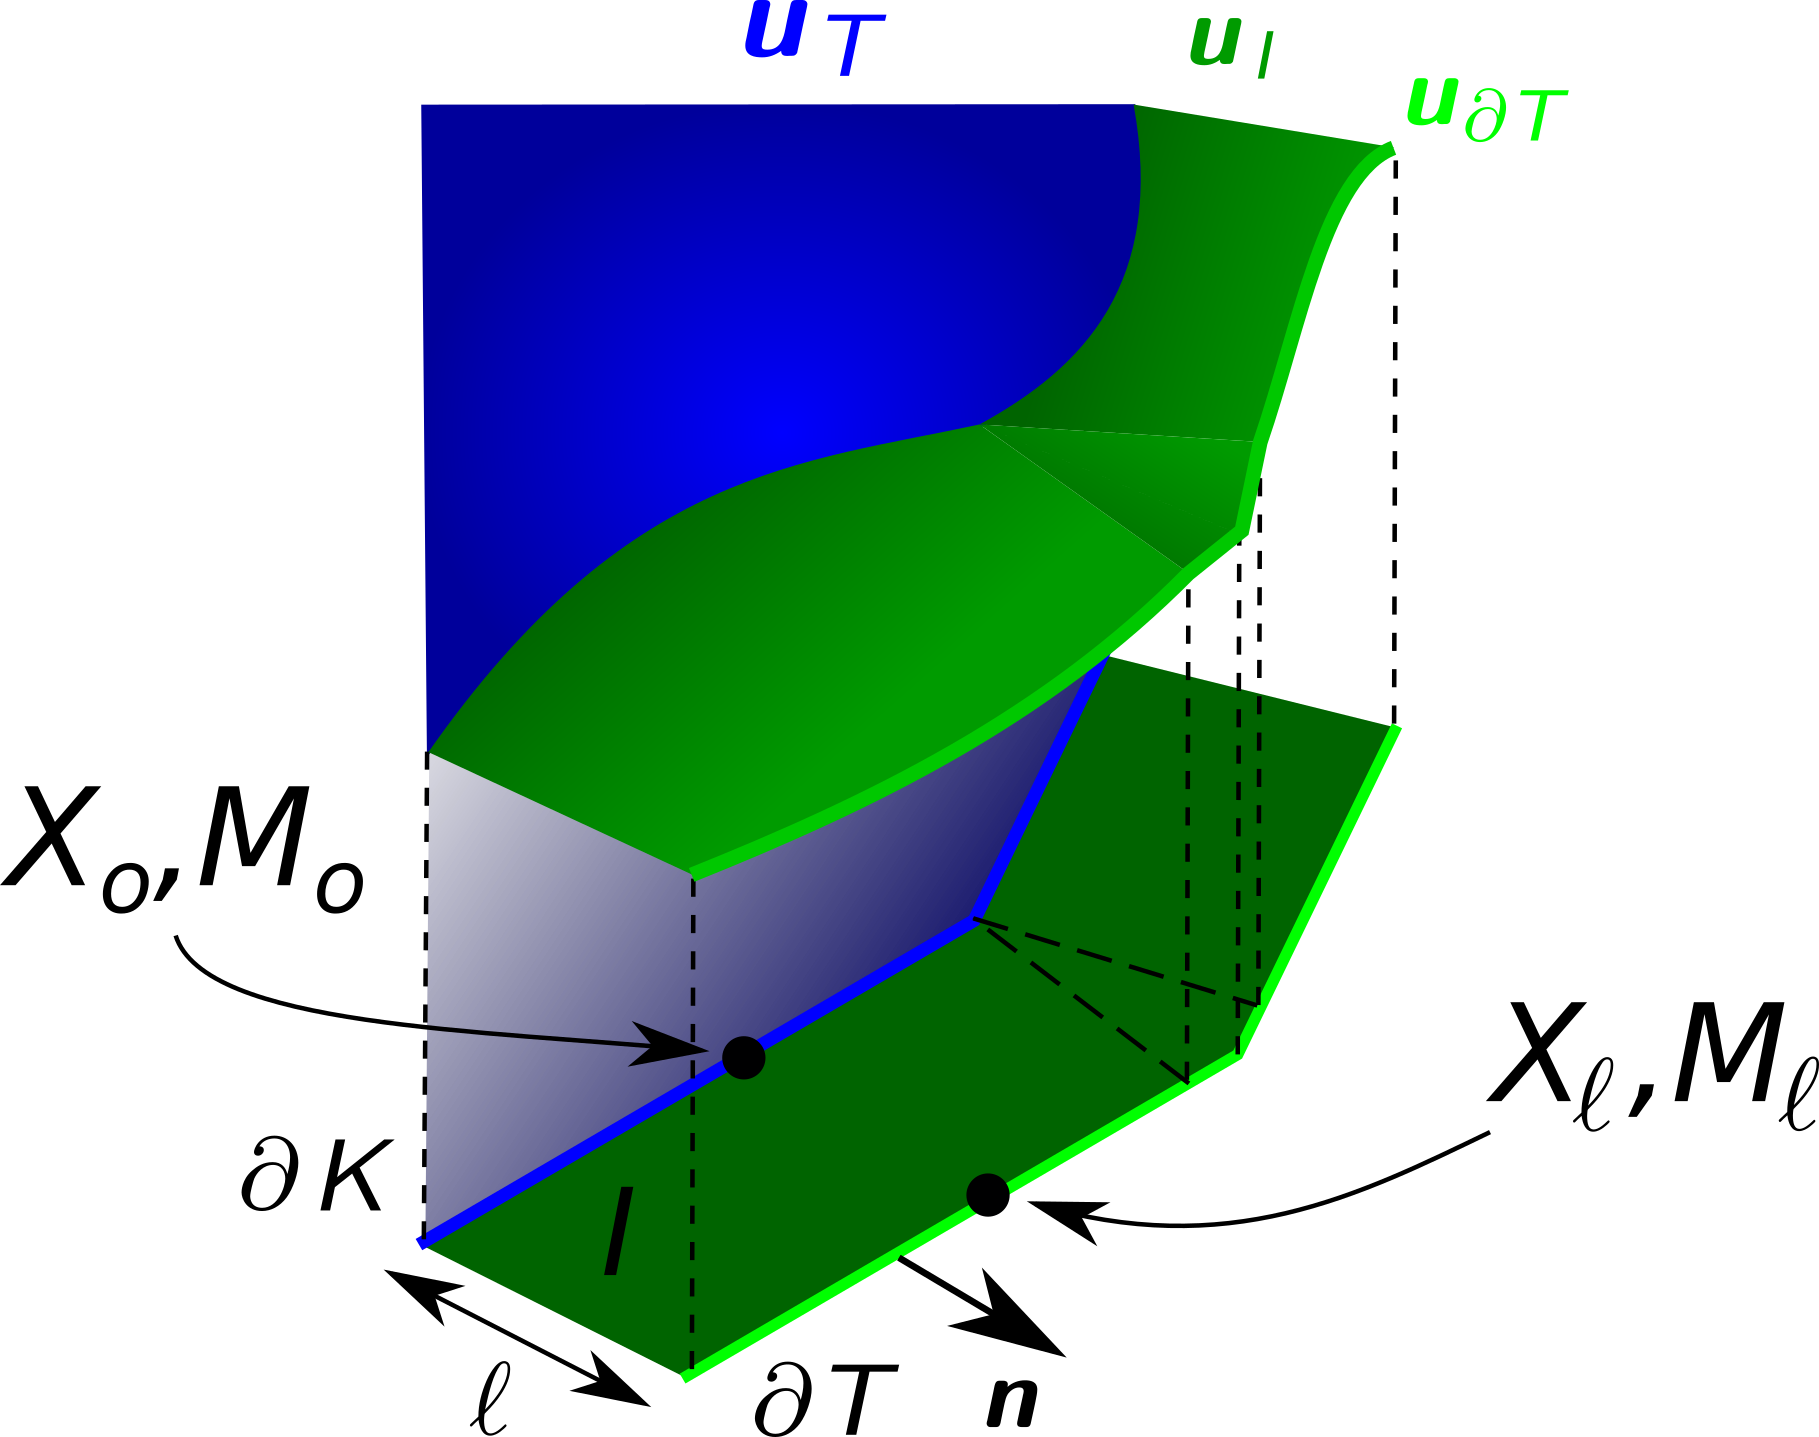
\includegraphics[width=7.cm]{../appendix/figures/yo.png}
    \caption{schematic representation of the cell, interface and boundary displacement fields close to a corner region}
    \label{fig_appendix_interface_displacement}
\end{figure}
%
%
%
\paragraph{Corners of a cell}

Since corners of the cell meet the intersection of two faces,
the displacement is assumed linear in the interface region around an intersection
such that it linearly bridges the displacement of the cell corner, to that of the two
faces tips (See Figure \ref{fig_appendix_interface_displacement}).
In the following, the corner region is supposed to be small compared to $\ell^2$, such that is is not considered in the following development.

% ---------------------------------------------------------
% PARAGRAPH
% ---------------------------------------------------------
\paragraph{Displacement gradient in the interface}

The derivative of $\tensori{u}{}_{\Crown{}}$ with respect to $\tensori{X}$ yields
%
%
%
\begin{equation}
    \frac{
        \partial \tensoro{u}{}_{\Crown{}i}
    }{
        \partial X_j
    }
    =
    \sum_k
    \frac{
        \partial \tensoro{u}{}_{\Crown{}i}
    }{
        \partial M_k
    }
    \frac{
        \partial M_k
    }{
        \partial X_j
    }
    =
    \frac{
    \tensoro{u}{}_{\dCell{}i}(\tensori{\Psi}{}^{-1}(\tensori{M}{}_{\ell}))
    -
    \tensoro{u}{}_{\Bulk{}i} \vert_{\dBulk{}}(\tensori{\Psi}{}^{-1}(\tensori{M}{}_{o}))
    }
    {\ell}
    Q_{0j}
\end{equation}
%
%
%
which reads
%
%
%
\begin{equation}
    \label{eq_grad_displacement_interface}
    \nabla \tensori{u}{}_{\Crown{}}(\tensori{X}) =
    \frac{
    \tensori{u}{}_{\dCell{}}(\tensori{X}{}_{\ell})
    -
    \tensori{u}{}_{\Bulk{}} \vert_{\dBulk{}}(\tensori{X}{}_{o})
    }
    {\ell}
    \otimes
    \tensori{n}{}
\end{equation}
%
%
%
where the fact that the first row of the rotation matrix $\tensorii{Q}$ is given by $\tensori{n}$ has been used. The points $\tensori{X}{}_{o}$ and $\tensori{X}{}_{\ell}$ are located on the normal plane to $\tensori{n}$ on $\dBulk{}$ and $\dCell{}$ respectively, in the reference frame.

% ---------------------------------------------------------
% PARAGRAPH
% ---------------------------------------------------------
\paragraph{Stress in the interface}

As introduced in Section \ref{sec_appendix_composite_demo}, the stress $\tensorii{P}{}_{\Crown}$ is assumed constant along the direction $\tensori{n}{}$ in $\Crown{}$. By continuity of the traction force across $\dBulk$, the following equality holds true
%
% 
% 
\begin{equation}
    \label{eq_continuity_traction_force_2}
    \begin{aligned}
        (\tensorii{P}{}_{\Crown} - \tensorii{P}{}_{\Bulk} \vert_{\dBulk{}}) \cdot \tensori{n}{} =  0
        &&
        \text{on}
        &&
        \dBulk{}
    \end{aligned}
\end{equation}

% ---------------------------------------------------------
% PARAGRAPH
% ---------------------------------------------------------
\paragraph{Internal Hu-Washizu in the interface}

Let $L_{\Crown{}, \text{int}}^{HW}$ the internal contribution of the Hu-Washizu Lagrangian in $\Crown{}$
%
%
%
\begin{equation}
    \label{eq22}
    \begin{aligned}
        L_{\Crown{}, \text{int}}^{HW}
        := &
        \int_{\Crown{}} \mecPotential{}_{\Crown} + \int_{\Crown{}} (\nabla \tensori{u}{}_{\Crown} - \tensorii{G}{}_{\Crown}) : \tensorii{P}{}_{\Crown}
    \end{aligned}
\end{equation}
%
% 
%
Let $C_\Crown = \{ v \in L^2(\Crown) \ \vert \ v \cdot \tensori{n} = \text{cste} \}$ the set of $L^2$-functions which are constant along the normal axis in $\Crown$. For any function in $C_\Crown$, the following equality holds true:
%
% 
% 
\begin{equation}
    \label{eq_virtual_works0}
        \int_{\Crown} v \ dV
        =
        \int_{\dBulk{}} \int_{\epsilon = 0}^{\ell} v (1 - \alpha \epsilon) \ dS d \epsilon
        =
        \ell (1 - \frac{\alpha}{2} \ell) \int_{\dBulk{}} v \ dS
\end{equation}
%
% 
% 
Noticing that $\nabla \tensori{u}{}_{\Crown} \in C_\Crown$, one has :
%
% 
% 
\begin{equation}
    \begin{aligned}
        \int_{\Crown{}} \mecPotential{}_{\Crown}
        = & 
        \ell (1 - \frac{\alpha}{2} \ell)
        \int_{\dBulk{}} \frac{1}{2} \beta \frac{\ell}{h_{\cell}} \nabla \tensori{u}{}_{\Crown} : \nabla \tensori{u}{}_{\Crown}
        \\
        = & 
        \ell (1 - \frac{\alpha}{2} \ell)
        \int_{\dBulk{}} \frac{\beta}{2 \ell h_{\cell}} (\tensori{u}{}_{\dCell} - \tensori{u}{}_{\Bulk} \vert_{\dBulk}) \otimes
        \tensori{n} : (\tensori{u}{}_{\dCell} - \tensori{u}{}_{\Bulk} \vert_{\dBulk}) \otimes
        \tensori{n}
        \\
        = & 
        \ell (1 - \frac{\alpha}{2} \ell)
        \int_{\dBulk{}} \frac{\beta}{2 \ell h_{\cell}} \lVert \tensori{u}{}_{\dCell} - \tensori{u}{}_{\Bulk}{} \vert_{\dBulk} \lVert {}^2
        \\
        = & 
        (1 - \frac{\alpha}{2} \ell)
        \int_{\dBulk{}} \frac{\beta}{2 h_{\cell}} \lVert \tensori{u}{}_{\dCell} - \tensori{u}{}_{\Bulk}{} \vert_{\dBulk} \lVert {}^2
    \end{aligned}
\end{equation}
%
% 
% 
Moreover, for $\tensorii{P}{}_{\Crown}$ in $C_\Crown{}$ :
%
% 
% 
\begin{equation}
    \begin{aligned}
        \int_{\Crown{}} \nabla \tensori{u}{}_{\Crown} : \tensorii{P}{}_{\Crown}
        = &
        \ell (1 - \frac{\alpha}{2} \ell)
        \int_{\dBulk{}} \nabla \tensori{u}{}_{\Crown} : \tensorii{P}{}_{\Crown}
        \\
        = &
        \ell (1 - \frac{\alpha}{2} \ell)
        \int_{\dBulk{}}
        \frac{1}{\ell}
        (\tensori{u}{}_{\dCell} - \tensori{u}{}_{\Bulk}{} \vert_{\dBulk}) \otimes \tensori{n} : \tensorii{P}{}_{\Crown{}}
        \\
        = &
        (1 - \frac{\alpha}{2} \ell)
        \int_{\dBulk{}}
        (\tensori{u}{}_{\dCell} - \tensori{u}{}_{\Bulk}{} \vert_{\dBulk}) \cdot \tensorii{P}{}_{\Bulk{}} \vert_{\dBulk{}} \cdot \tensori{n}
    \end{aligned}
\end{equation}
% 
% 
% 
where \eqref{eq_continuity_traction_force_2} has been used. And Finally :
%
% 
% 
\begin{equation}
    \begin{aligned}
        L_{\Crown{}, \text{int}}^{HW}
        =
        (1 - \frac{\alpha}{2} \ell)
        \int_{\dBulk{}} \frac{\beta}{2 h_{\cell}} \lVert \tensori{u}{}_{\dCell{}} - \tensori{u}{}_{\Bulk{}} \vert_{\dBulk{}} \rVert^2
        +
        (1 - \frac{\alpha}{2} \ell)
        \int_{\dBulk} (\tensori{u}{}_{\dCell{}} - \tensori{u}{}_{\Bulk{}} \vert_{\dBulk{}}) \cdot \tensorii{P}{}_{\Bulk{}} \vert_{\dBulk{}} \cdot \tensori{n}{}
        -
        \int_{\Crown{}} \tensorii{G}{}_{\Crown{}} : \tensorii{P}{}_{\Crown{}}
    \end{aligned}
\end{equation}

% ---------------------------------------------------------
% PARAGRAPH
% ---------------------------------------------------------
\paragraph{Total Hu-Washizu Lagrangian in the composute element}

Injecting \eqref{eq22} in \eqref{eq_hu_washizu_split} yields
%
% 
% 
\begin{equation}
    \label{eq_0014}
    \begin{aligned}
        L_{\cell}^{HW}
        = &
        \int_{\Bulk} \mecPotential{}_{\bodyLag{}} + (\nabla \tensori{u}{}_{\Bulk} - \tensorii{G}{}_{\Bulk}) : \tensorii{P}{}_{\Bulk}
        % \\
        % &
        +
        (1 - \frac{\alpha}{2} \ell)
        % \Biggl(
        \int_{\dBulk{}} (\tensori{u}{}_{\dCell{}} - \tensori{u}{}_{\Bulk} \vert_{\dBulk}) \cdot \tensorii{P}{}_{\Bulk} \vert_{\dBulk} \cdot \tensori{n}{}
        % \\
        % &
        \\
        &
        +
        (1 - \frac{\alpha}{2} \ell)
        \int_{\dBulk{}} \frac{\beta}{2 h_T} \lVert \tensori{u}{}_{\dCell{}} - \tensori{u}{}_{\Bulk} \vert_{\dBulk{}} \rVert^2
        % \Biggr)
        % \\
        % &
        -
        \int_{\Crown{}} \tensorii{G}{}_{\Crown{}} : \tensorii{P}{}_{\Crown{}}
        % \\
        % &
        -
        \int_{\Bulk} \loadLag \cdot \tensori{u}{}_{\Bulk}
        -
        \int_{\Crown{}} \loadLag \cdot \tensori{u}{}_{\Crown{}}
        -
        \int_{\neumannCell{}} \neumannCellLoad{} \cdot \tensori{u}{}_{\dCell{}}
    \end{aligned}
\end{equation}
%
% 
% 
Since $\ell$ is arbitrary, let $\ell \rightarrow 0$,
the interface region vanishes such that $\Crown{} \rightarrow \emptyset, \Bulk{} \rightarrow \cell$ and $\dBulk{} \rightarrow \dCell$, and the expression of the Hu–Washizu functional over the region $\cell$ writes
% 
% 
%
\begin{equation}
    \label{eq_0015A}
    \begin{aligned}
        L_{\cell}^{HW}
        = &
        \int_{\cell{}} \mecPotential{}_{\bodyLag{}} + (\nabla \tensori{u}{}_{\cell{}} - \tensorii{G}{}_{\cell{}}) : \tensorii{P}{}_{\cell}
        % \\
        % &
        + \int_{\dCell{}} (\tensori{u}{}_{\dCell} - \tensori{u}{}_{\cell} \vert_{\dCell}) \cdot \tensorii{P}{}_{\cell} \vert_{\dCell{}} \cdot \tensori{n}{}
        % \\
        % &
        + \int_{\dCell} \frac{\beta}{2 h_{\cell}} \lVert \tensori{u}{}_{\dCell{}} - \tensori{u}{}_{\cell{}} \vert_{\dCell{}} \rVert^2
        \\
        &
        -
        \int_{\cell} \loadLag{} \cdot \tensori{u}{}_{\cell{}}
        -
        \int_{\neumannCell{}} \neumannCellLoad{} \cdot \tensori{u}{}_{\dCell{}}
    \end{aligned}
\end{equation}
%
%
%
which concludes the development of equation \eqref{eq_0015}.

\chapter{Implementation}
% ---------------------------------------------------------
% ---- SECTION
% ---------------------------------------------------------
\section{Implementation}
\label{sec_appendix_implementation}

This section specifies implementation aspects regarding HDG methods, and in particular those defining the HHO method.

% ---------------------------------------------------------
% -- SUBSECTION
% ---------------------------------------------------------
\subsection{Shape functions}
\label{sec_shape_functions}

Since the displacement is discontinuous, the usual Lagrange basis functions are not necessarily needed for the description of the discrete displacement, gradient ans stress fields. A natural choice amounts to choose monomial basis functions.

% ---------------------------------------------------------
% PARAGRAPH
% ---------------------------------------------------------
\paragraph{Monomial basis functions}

Let $\mathcal{M}_s^l$ the set of natural integer vectors in a $s$-dimensional euclidean space such that
%
%
%
\begin{equation}
    \begin{aligned}
        \mathcal{M}_s^l =
        % \{
        \bigg\{
            \mathcal{M}_{s,p} && \vert && 0 \leq p \leq l
        \bigg\}
        &&
        \text{with}
        &&
        \mathcal{M}_{s,p} =
        \bigg\{
            \tensori{\alpha}{}_m && \vert && \sum_{1 \leq j \leq s} \alpha_{mj} = p
        \bigg\}
        % \}
    \end{aligned}
\end{equation}
%
%
%
and denote $M_s^l$ the cardinality of $\mathcal{M}_s^l$.
Let $D$ some $s$-dimensional euclidean domain, $1 \leq s \leq 3$, and $M^l(D)$ the monomial basis function of order $l$ on $D$.
The value of a scalar polynomial field $a_{M}^l \in M^l(D)$ at some point $\tensori{X} \in D$ is given by
%
%
%
\begin{equation}
    \label{eq_basis_fun3}
    \begin{aligned}
        a_{M}^l(\tensori{X}) = \sum_{0 \leq p \leq M_s^l} a_{p} \prod_{1 \leq j \leq s} \frac{(X_j - X_{Dj})^{\alpha_{pj}}}{h_D}
        &&
        \text{with}
        &&
        \tensori{\alpha}{}_p \in \mathcal{M}_{s}^l
    \end{aligned}
\end{equation}
%
%
%
where $\tensori{X}{}_D$ denotes the centroid of $D$, and the coefficients $a_p$ in $M^l(D)$ form a vector $\mathfrak{A}_D^l$ of size $M_s^l$.

% ---------------------------------------------------------
% PARAGRAPH
% ---------------------------------------------------------
\paragraph{Cell and faces approximation space sizes}

The number of degrees of freedom for a scalar field depends on the polynomial order. An overview of the values taken using monomial shape functions is given in tables \ref{table_num_dofs_2D} and \ref{table_num_dofs_3D} for both a cell and a face up to an approximation of order $4$
%
%
%
\begin{table}[H]
\centering
\begin{tabular}{||c c c||} 
    \hline
    polynomial order & cell dofs & face dofs \\ [0.5ex] 
    \hline\hline
    $0$ & 1 & 1
    \\ \hline
    $1$ & 3 & 2
    \\ \hline
    $2$ & 6 & 3
    \\ \hline
    $3$ & 10 & 4
    \\ \hline
    $4$ & 15 & 5
    \\ \hline
\end{tabular}
\caption{Number of cell and faces degrees of freedom for a scalar unknown in two dimension}
\label{table_num_dofs_2D}
\end{table}
%
%
%
\begin{table}[H]
\centering
\begin{tabular}{||c c c||} 
    \hline
    polynomial order & cell dofs & face dofs \\ [0.5ex] 
    \hline\hline
    $0$ & 1 & 1
    \\ \hline
    $1$ & 4 & 3
    \\ \hline
    $2$ & 10 & 6
    \\ \hline
    $3$ & 19 & 10
    \\ \hline
    $4$ & 35 & 15
    \\ \hline
\end{tabular}
\caption{Number of cell and faces degrees of freedom for a scalar unknown in three dimension}
\label{table_num_dofs_3D}
\end{table}
%
%
%
The need to eliminate cell unknowns justifies by observing that the number of degrees of freedom in cells grows rapidly with the approximation order as compared to that in faces.

% ---------------------------------------------------------
% -- SUBSECTION
% ---------------------------------------------------------
\subsection{Stabilization}
\label{sec_stabilization}

In this section, approximation spaces for unknowns of the global problem are described, which leads to several choices in terms of definition of the jump function. Depending on such a choice, one recovers either the HDG method as defined by \cite{lehrenfeld_hdg_2010}, or the HHO \cite{di_pietro_hybrid_2015} one.

% ---------------------------------------------------------
% PARAGRAPH
% ---------------------------------------------------------
\paragraph{Discrete functional space}

Discrete spaces are chosen such that
%
%
%
\begin{equation*}
    \begin{aligned}
        \discreteDisplacementSpaceCell = P^l(\cell, \mathbb{R}^{d})
        &&
        \discreteDisplacementSpaceDCell = P^k(\dCell, \mathbb{R}^{d})
        &&
        \discreteGradSpaceCell = P^k(\cell, \mathbb{R}^{d \times d})
        &&
        \discreteStressSpaceCell = P^k(\cell, \mathbb{R}^{d \times d})
    \end{aligned}
\end{equation*}
%
%
%
where $P^a(D, \mathbb{R}^{m})$ denotes the space of $m-$ valued polynomials in $D$, spanned by the monomial basis $M^a(D)$. In particular, one notices that the cell displacement polynomial order $l$ might be chosen different from the face displacement order $k$ such that $k - 1 \leq l \leq k + 1$.

% ---------------------------------------------------------
% PARAGRAPH
% ---------------------------------------------------------
\paragraph{HDG jump function}

Accounting for the possible different polynomial order between the cell and faces, one can specify a discrete jump function (or stabilization) in a straightforward way such that it delivers the displacement difference point-wise for any displacement pair $(\tensori{v}{}_{\cell}^l, \tensori{v}{}_{\dCell}^k) \in U^h(\cell) \times V^h(\dCell)$
%
%
%
\begin{equation}
    \begin{aligned}
        \tensori{J}{}_{\dCell}^{HDG}(\tensori{v}{}_{\cell}^l, \tensori{v}{}_{\dCell}^k) = \Pi^k_{\dCell{}} (
            \tensori{v}{}_{\dCell}^k - \tensori{v}{}_{\cell}^l \vert_{\dCell}
        )
    \end{aligned}
\end{equation}
%
%
%
where $\Pi^k_{\dCell{}}$ denotes the orthogonal projector onto $\discreteDisplacementSpaceDCell$.
This discrete jump function is at the origin of Hybrid Discontinuous Galerkin methods \cite{lehrenfeld_hdg_2010}, and grants a convergence of order $k$ in the energy norm.

% ---------------------------------------------------------
% PARAGRAPH
% ---------------------------------------------------------
\paragraph{HHO jump function}

A richer discrete jump function $\tensori{J}{}_{\dCell}^{HHO}$ providing a convergence of order $k + 1$ in the energy norm was introduced in \cite{di_pietro_discontinuous-skeletal_2015}, hence giving the Hybrid High Order method its name, such that
%
%
%
\begin{equation}
    \label{eq_hho_stabilization_vector}
    \begin{aligned}
        \tensori{J}{}_{\dCell}^{HHO}(\tensori{v}{}_{\cell}^l, \tensori{v}{}_{\dCell}^k) = \Pi^k_{\dCell{}} (
            \tensori{v}{}_{\dCell}^k - \tensori{v}{}_{\cell}^l \vert_{\dCell}
            -
            (
                (\tensoro{I}{}_{\cell}^{k + 1} - \Pi_{\cell}^k) (
                    \tensori{w}{}_\cell^{k + 1}
                )
            ) \vert_{\dCell{}}
        )
    \end{aligned}
\end{equation}
%
%
%
where $\Pi_{\cell}^k$ is the projector onto $P^{k}(\cell, \mathbb{R}^{d})$, $\tensoro{I}{}_{\cell}^{k + 1}$ is the identity function in $\discretePotentialSpaceCell = P^{k + 1}(\cell, \mathbb{R}^{d})$.

% ---------------------------------------------------------
% PARAGRAPH
% ---------------------------------------------------------
\paragraph{Reconstructed higher order displacement}

The term $\tensori{w}{}_{\cell}^{k+1}$ in \eqref{eq_hho_stabilization_vector}
% $ \in \discretePotentialSpaceCell$
denotes a higher order discrete displacement in $\discretePotentialSpaceCell$ that solves for any displacement pair $(\tensori{v}{}_{\cell}^l, \tensori{v}{}_{\dCell}^k) \in U^h(\cell) \times V^h(\dCell)$
%
%
%
\begin{subequations}
    \label{eq_potential}
        \begin{alignat}{3}
            \int_\cell \nabla \tensori{w}{}_{\cell}^{k+1} : \nabla \tensori{d}{}_{\cell}^{k+1}
            & =
            \int_\cell \nabla \tensori{v}{}_{\cell}^l : \nabla \tensori{d}{}_{\cell}^{k+1}
            +
            \int_{\dCell} (\tensori{v}{}_{\dCell}^k - \tensori{v}{}_{\cell}^l) \cdot \nabla \tensori{d}{}_{\cell}^{k+1} \cdot \tensori{n}{}
            \ \ \ \ \ \ \ \ 
            &&
            \forall \tensori{d}{}_{\cell}^{k+1} \in \discretePotentialSpaceCell
            \label{eq_potential:eq0}
            \\
            \int_\cell \tensori{w}{}_{\cell}^{k+1} & = \int_\cell \tensori{v}{}_{\cell}^{l}
            \label{eq_potential:eq1}
    \end{alignat}
\end{subequations}

% ---------------------------------------------------------
% -- SUBSECTION
% ---------------------------------------------------------
\subsection{Algebraic formulation}
\label{sec_appendix_implementation2}

% ---------------------------------------------------------
% PARAGRAPH
% ---------------------------------------------------------
\paragraph{Unknown vector}

A cell displacement component unknown is represented by the coefficient vector $\mathfrak{U}_{\cell}^l$ in $M^l(\cell)$, and a face displacement component unknown is represented by the coefficient vector $\mathfrak{U}_{F}^k$ in $M^k(F)$, for any $F \subset \dCell$.
The global element displacement unknown vector of size $d M^l_d + d N_{\dCell} M^k_{d - 1}$ is
denoted $\mathfrak{U}_{\ClosedCell{}}$ and is the collection of all cell and faces displacement component vectors.
In the following, the cell coefficients in $\mathfrak{U}_{\ClosedCell{}}$ are denoted $\mathfrak{U}_{\cell}$, and the boundary coefficients $\mathfrak{U}_{\dCell}$.

% ---------------------------------------------------------
% PARAGRAPH
% ---------------------------------------------------------
\paragraph{Quadrature}

Integrals are evaluated numerically by means of a quadrature rule on an element shape. Hence, let ${Q}_D$ a quadrature rule for the domain $D$ of order at least $2k$. A quadrature point is denoted $\tensori{X}{}_q$ and a quadrature weight $w_q$.

% ---------------------------------------------------------
% PARAGRAPH
% ---------------------------------------------------------
\paragraph{Reconstructed gradient operator}

From an algebraic standpoint, \eqref{eq_grad} defines a linear problem
consisting in inverting a mass matrix in $\discreteGradSpaceCell{}$. One can thus define 
$
{\mathbb{B}}{}_{\cell}
$
the discrete gradient operator acting on the displacement unknowns vector $\mathfrak{U}{}_{\ClosedCell}$ at a quadrature point $\tensori{X}{}_q \in \cellQuadrature$, and ${\mathfrak{G}}{}_{\cell}^k$ the vector representation of the reconstructed gradient $\tensorii{G}{}_{\cell}^k(\tensori{v}{}_{\cell}^l, \tensori{v}{}_{\dCell}^k)$ such that
%
%
%
\begin{equation}
    \label{eq_discrete_gradient_vector}
    \begin{aligned}
        {\mathfrak{G}}{}_{\cell}^k
        (\tensori{X}{}_q)
        =
        {\mathbb{B}}{}_{\cell}
        (\tensori{X}{}_q)
        \cdot
        {\mathfrak{U}}{}_{\ClosedCell}
    \end{aligned}
\end{equation}
%
%
%
where ${\mathbb{B}}{}_{\cell}$ is composed by a cell block and a boundary block of respective size $dM_d^l$ and $dM_{d - 1}^k$.

% ---------------------------------------------------------
% PARAGRAPH
% ---------------------------------------------------------
\paragraph{Stabilization operator}

Similarly, the algebraic realization of \eqref{eq_hho_stabilization_vector} amounts to compute the stabilization operator ${\mathfrak{J}}{}_{\cell}$ such that 
%
%
%
\begin{equation}
    \label{eq_discrete_stabilization_vector}
    \begin{aligned}
        % {\mathcal{J}}{}_{\dCell}^{HHO}
        {\mathfrak{J}}{}_{\dCell}^{HHO}
        =
        {\mathbb{J}}{}_{\cell}
        \cdot
        {\mathfrak{U}}{}_{\ClosedCell}
    \end{aligned}
\end{equation}
%
%
%
where, as for ${\mathbb{B}}{}_{\cell}$, the operator ${\mathbb{J}}{}_{\cell}$ is composed by a cell and a boundary block with same respective sizes.

% ---------------------------------------------------------
% PARAGRAPH
% ---------------------------------------------------------
\paragraph{Offline computation}

Since \eqref{eq_grad} and \eqref{eq_hho_stabilization_vector} depend on the geometry of the element $\cell$ only, one can compute the operators $\mathbb{B}{}_{\cell}$ and $\mathbb{Z}{}_{\cell}$ for each element once and for all in an offline pre-computation step by working in the reference configuration. Once this offline step is performed, the algebraic form of the problem resembles closely to the standard finite element one, where the operator $\mathbb{B}{}_{\cell}$ replaces the usual shape function gradient operator, and the stabilization operator 
$\mathbb{Z}{}_{\cell}$ is incorporated in the expression of the tangent matrix and in that of internal forces.

% ---------------------------------------------------------
% PARAGRAPH
% ---------------------------------------------------------
\paragraph{Internal forces} The internal forces vector $\mathfrak{F}_{\ClosedCell}^{int}$ depends on the product of the stress values with the gradient operator computed at quadrature points, plus a supplementary force corresponding to that of the traction between the cell and its boundary
%
%
%
\begin{equation}
    \label{eq_internal_forces}
    \begin{aligned}
    \mathfrak{F}_{\ClosedCell}^{int}
    % (\mathfrak{U}{}_{\ClosedCell})
    = &
    \sum_{\tensori{X}{}_q \in \cellQuadrature{}}
    (w_q
    {\mathbb{B}}{}_{\cell}^{t}(\tensori{X}{}_q) \cdot
    {\mathfrak{P}}{}_{\cell}^k(\tensori{X}{}_q, \mathfrak{U}{}_{\ClosedCell})
    )
    +
    \frac{\beta}{h_T}
    {\mathbb{J}}{}_{\cell}^t
    \cdot
    {\mathbb{J}}{}_{\cell}
    \cdot
    {\mathfrak{U}}{}_{\ClosedCell}
    \end{aligned}
\end{equation}
%
%
%
where ${\mathfrak{P}}{}_{\cell}^k$ denotes the vector representation of $\tensorii{P}{}_{\cell}^k$, and the superscript $\{\cdot\}^t$ denotes the transposition operator.

% ---------------------------------------------------------
% PARAGRAPH
% ---------------------------------------------------------
\paragraph{External forces}

The external forces vector $\mathfrak{F}_{\ClosedCell}^{ext}$ is the evaluation of the given bulk and boundary loads at respective cell and face quadrature points tested against the respective cell and face shape functions, such that
%
%
%
\begin{equation}
    \label{eq_external_forces}
    \begin{aligned}
        \mathfrak{F}_{\cell}^{ext}
        =
        \sum_{\tensori{X}{}_q \in \cellQuadrature{}}
        (w_q
        \loadLag{}(\tensori{X}{}_q) \cdot
        {\mathfrak{U}}{}_{\cell}^l
        )
        &&
        \text{and}
        &&
        \mathfrak{F}_{\dCell}^{ext}
        =
        \sum_{\tensori{X}{}_q \in Q_{\dCell}}
        (w_q
        \neumannLag{}(\tensori{X}{}_q) \cdot
        {\mathfrak{U}}{}_{\dCell}^k
        )
    \end{aligned}
\end{equation}

% ---------------------------------------------------------
% PARAGRAPH
% ---------------------------------------------------------
\paragraph{Tangent matrix and resiudal}

The elementary residual vector $\mathfrak{R}_{\ClosedCell}$ is such
that $\mathfrak{R}_{\ClosedCell} =
\mathfrak{F}_{\ClosedCell}^{int} -
\mathfrak{F}_{\ClosedCell}^{ext}$. The tangent matrix
$\mathbb{K}_{\ClosedCell}$ expresses the
derivative of $\mathfrak{R}_{\ClosedCell}$
with respect to $\mathfrak{U}{}_{\ClosedCell}$, and writes such that
%
%
%
\begin{equation}
  \label{eq_stiffness_operator}
  \begin{aligned}
    \mathbb{K}_{\ClosedCell}
    = \sum_{\tensori{X}{}_q \in \cellQuadrature{}} (w_q
    {\mathbb{B}}{}_{\cell}^{t}(\tensori{X}{}_q) \cdot
    \mathbb{A}(\tensori{X}{}_q, \mathfrak{U}{}_{\ClosedCell}) \cdot
    {\mathbb{B}}{}_{\cell}(\tensori{X}{}_q) ) + \frac{\beta}{h_T}
    {\mathbb{J}}{}_{\cell}^t \cdot {\mathbb{J}}{}_{\cell}
  \end{aligned}
\end{equation}
%
%
%
where $\mathbb{A}$ is the matrix representation of the
fourth-order tensor $\tensoriv{A}{} = \partial \tensorii{P}{}_{\cell}^k
/ \partial \tensorii{G}{}_{\cell}^k$. The matrix
$\mathbb{K}_{\ClosedCell}$ is block
decomposable such that
%
%
%
\begin{equation}
  \label{eq_stiffness_operator_blocks}
  \begin{aligned}
    \mathbb{K}_{\ClosedCell}
    =
    \begin{pmatrix}
      \mathbb{K}_{\cell
        \cell} && \mathbb{K}_{\cell
        \dCell} \\
      \mathbb{K}_{\dCell
        \cell} && \mathbb{K}_{\dCell
        \dCell}
    \end{pmatrix}
  \end{aligned}
\end{equation}
%
%
%
which leads to the following algebraic expression of
both~\eqref{eq_cell_equilibrium_3}
and~\eqref{eq_static_condensation_final}~:
\begin{equation}
  \label{eq_condensation_matrix}
  \begin{aligned}
    \frac{d \mathfrak{R}_{\mathcal{F}}}{d
      \mathfrak{U}_{\mathcal{F}}} = \frac{d
      \mathfrak{R}_{\mathcal{F}}^c}{d \mathfrak{U}_{\mathcal{F}}} =
    \mathbb{K}_{\cell \dCell} -
    \mathbb{K}_{\dCell \cell}
    \mathbb{K}_{\cell \cell}^{-1}
    \mathbb{K}_{\cell \dCell}
  \end{aligned}
\end{equation}

% ---------------------------------------------------------
% -- SUBSECTION
% ---------------------------------------------------------
\subsection{Operators in the axi-symmetric framework}
\label{sec_appendix_axi}

This part specifies the formulation of HHO operators in the axi-symmetric framework.

% ---------------------------------------------------------
% PARAGRAPH
% ---------------------------------------------------------
\paragraph{Reconstructed gradient}

For any displacement pair $(\tensori{v}{}_{\cell}^l, \tensori{v}{}_{\dCell}^k) \in \discreteDisplacementSpaceCell{} \times \discreteDisplacementSpaceDCell{}$, the component $\tensoro{G}{}_{\cell \theta \theta}(\tensoro{v}{}_{\cell r}, \tensoro{v}{}_{\dCell r})$ solves
%
%
%
\begin{equation}
    \label{axi_symmetric_gradient_theta}
    \begin{aligned}
        \int_{\cell} 2 \pi r \tensoro{G}{}_{\cell \theta \theta}(\tensoro{v}{}_{\cell r}, \tensoro{v}{}_{\dCell r}) \tensoro{\tau}{}_{\cell \theta \theta}
        =
        \int_{\cell} 2 \pi r \frac{\tensoro{u}{}_{\cell r}}{r} \tensoro{\tau}{}_{\cell \theta \theta}
        =
        \int_{\cell} 2 \pi \tensoro{u}{}_{\cell r} \tensoro{\tau}{}_{\cell \theta \theta}
        &&
        \forall \tensorii{\tau}{}_{\cell} \in \stressSpaceCell
    \end{aligned}
\end{equation}
%
%
%
In the radial and ordonal directions, \textit{i.e.} $\forall i, j \in \{ r,z \}$, the expression given in \eqref{eq_grad} is retrieved, and the component $G_{\cell ij}(\tensoro{v}{}_{\cell i}, \tensoro{v}{}_{\dCell i})$ solves
%
%
%
\begin{equation}
    \label{axi_symmetric_gradient_rz}
    \begin{aligned}
    \int_{\cell} 2 \pi r G_{\cell ij}(\tensoro{v}{}_{\cell i}, \tensoro{v}{}_{\dCell i}) \tau_{\cell ij} =
    \int_{\cell} 2 \pi r \frac{\partial \tensoro{u}{}_{\cell i}}{\partial j} \tau_{ij} -
    \int_{\dCell} 2 \pi r (u_{\dCell i} - u_{\cell i} \vert_{\dCell}) \tau_{\cell ij} \vert_{\dCell} n_{j}
    &&
    \forall \tensorii{\tau}{}_{\cell} \in \stressSpaceCell
    \end{aligned}
\end{equation}

% ---------------------------------------------------------
% PARAGRAPH
% ---------------------------------------------------------
\paragraph{Reconstructed higher order displacement}

For any $\tensori{d}{}_{\cell}^{k + 1} \in \discretePotentialSpaceCell$, the radial component $w^{k+1}_{\cell r}$ solves
%
%
%
\begin{equation}
    \label{axi_symmetric_potential_r}
    \begin{aligned}
        \int_{\cell} 2 \pi r (\sum_{i \in \{ r,z \}} \frac{\partial w^{k+1}_{\cell r}}{\partial i} \frac{\partial d^{k+1}_{\cell r}}{\partial i} + \frac{w^{k+1}_{\cell r}}{r} \frac{d^{k+1}_{\cell r}}{r})
        = &
        \int_{\cell} 2 \pi r (\sum_{i \in \{ r,z \}} \frac{\partial u_{\cell r}}{\partial i} \frac{\partial d^{k+1}_{\cell r}}{\partial i} + \frac{u_{\cell r}}{r} \frac{d^{k+1}_{\cell r}}{r})
        \\
        &
        +
        \int_{\dCell} 2 \pi r \sum_{i \in \{ r,z \}} (u_{\dCell r} - u_{\cell r} \vert_{\dCell}) \frac{\partial d^{k+1}_{\cell r}}{\partial i} \vert_{\dCell} n_{i}
    \end{aligned}
\end{equation}
%
%
%
where the mean value condition is not needed on the radial component of the higher order displacement since the left hand side of the system described by \eqref{axi_symmetric_potential_r} depends directly on the displacement unknown and not only on its gradient as in \eqref{axi_symmetric_potential_z}.
The ordinate component $w^{k+1}_{\cell z}$ solves :
%
%
%
\begin{subequations}
    \label{axi_symmetric_potential_z}
        \begin{alignat}{3}
            \int_{\cell} 2 \pi r \sum_{i \in \{ r,z \}}
            \frac{\partial w^{k+1}_{\cell z}}{\partial i} \frac{\partial d^{k+1}_{\cell z}}{\partial i}
            = &
            \int_{\cell} 2 \pi r \sum_{i \in \{ r,z \}} \frac{\partial u_{\cell z}}{\partial i} \frac{\partial d^{k+1}_{\cell z}}{\partial i}
            -
            \int_{\dCell} 2 \pi r \sum_{i \in \{ r,z \}} (u_{\dCell z} - u_{\cell z} \vert_{\dCell})
            \frac{\partial d^{k+1}_{\cell z}}{\partial i} \vert_{\dCell} n_{i}
            \\
            \int_{\cell} 2 \pi r w^{k+1}_{\cell z} = & \int_{\cell} 2 \pi r u_{\cell z}
        \end{alignat}
\end{subequations}

\paragraph{Axis faces treatment}

In cylindrical coordinates, all integrals depend on the radial component $r$, and boundary integrals vanish at $r = 0$ on the symmetry axis.
As a consequence, some information on the boundary displacement is lost in the surface integral term of both the reconstructed gradient and the stabilization of a cell $\cell$ located on the symmetry axis.
% do not depend on the closed surface integral wrapping a cell $\cell$ located on the symmetry axis.
% Therefore, the reconstructed gradient (and the stabilization) do not depend on the closed surface integral wrapping a cell $\cell$ located on the symmetry axis.
However, this feature is necessary to prove the robustness of the HHO method to volumetric locking (see \ref{sec_appendix_gradient}).
In order to circumvent this problem, we consider infinitely thin cylindrical faces wrapping the symmetry axis, that are subjected to Dirichlet boundary conditions along the radial direction.
% Thus, in order to restore full mobility of a face located on the symmetry axis, we consider infinitely thin cylindrical faces wrapping it, that are subjected to Dirichlet boundary conditions along the radial direction.

% ---------------------------------------------------------
% ---- SECTION
% ---------------------------------------------------------
\section{Numerical examples in plane strain and tridimensional modelling hypotheses}
\label{sec_implementation_tridimensional_results}

The section showcases numerical examples demonstrating the robustness
of the cell resolution algorithm. The test cases under study, namely the
classical Cook membrane, and the indentation test cases, show that no
volumetric locking is encountered using the cell resolution algorithm.

% ---------------------------------------------------------
% -- SUBSECTION
% ---------------------------------------------------------
\subsection{Cook's membrane test case}

% ---------------------------------------------------------
% PARAGRAPH
% ---------------------------------------------------------
\paragraph{Specimen and loading}

Let consider the Cook membrane specimen that is subjected to uniaxial
traction. The membrane has a width of $48$ mm and a height of $60$ mm,
and a vertical traction $t_y = 1000$ N/m is imposed at the top. The HHO
computation is run on a polygonal mesh (see Figure \ref{fig_cook}) and
is compared with standard QU4 and QU8 formulations (\textit{i.e.} linear
and quadratic approximations)

% ---------------------------------------------------------
% PARAGRAPH
% ---------------------------------------------------------
\paragraph{Constitutive equation}

The same behavior law as that in \ref{sec_swelling_sphere} is
considered for the present test case. However, the finite strain
hypothesis is chosen, based on a logarithmic decomposition of the stress
\cite{miehe_anisotropic_2002}.

% ---------------------------------------------------------
% PARAGRAPH
% ---------------------------------------------------------
\paragraph{Material parameters}

Materials parameters are taken as
$\sigma_0 = 450$ MPa, $\sigma_{\infty} = 715$ MPa with a saturation parameter $\delta = 16.93$. The Young modulus is $E = 206.9$ GPa, and the Poisson ratio is $\nu = 0.29$.

\begin{figure}[H]
    \centering
    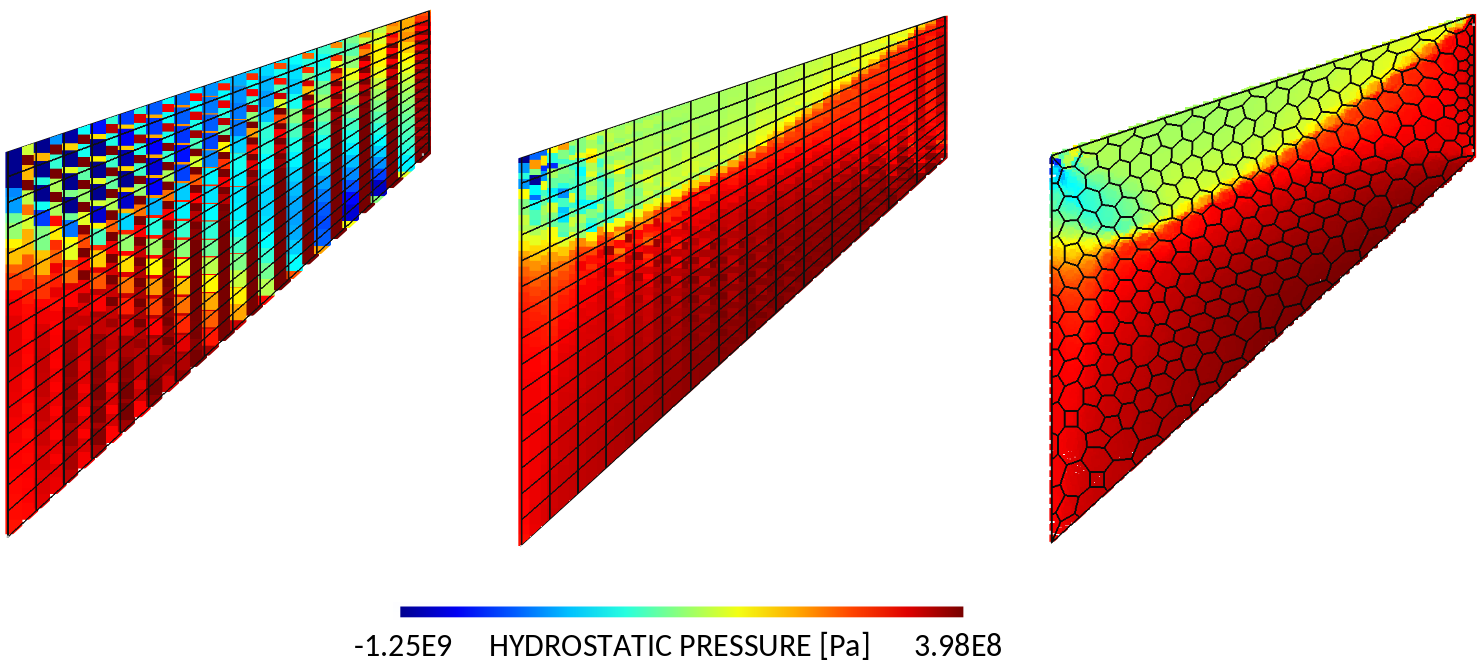
\includegraphics[width=12.cm]{../chapter_01_hho_mechanics/figures/cook_comp.png}
    \caption{Hydrostatic pressure map one the reference configuration at the limit load}
    \label{fig_cook}
\end{figure}

% ---------------------------------------------------------
% PARAGRAPH
% ---------------------------------------------------------
\paragraph{Numerical results}

As expected, the linear and quadratic finite element methods display respectively strong and mild oscillations of the pressure, whereas the HHO one shows no sign of locking.

% ---------------------------------------------------------
% -- SUBSECTION
% ---------------------------------------------------------
\subsection{Indentation test case}

% ---------------------------------------------------------
% PARAGRAPH
% ---------------------------------------------------------
\paragraph{Specimen and loading}

The last test case consists in the indentation of a cube of size $10$ mm. A pressure of $300$ MPa is imposed on the top surface see Figure \ref{fig_cube}).

% ---------------------------------------------------------
% PARAGRAPH
% ---------------------------------------------------------
\paragraph{Material}

The same perfect plastic material as that in \ref{sec_swelling_sphere} is considered for the present test case.

\begin{figure}[H]
    \centering
    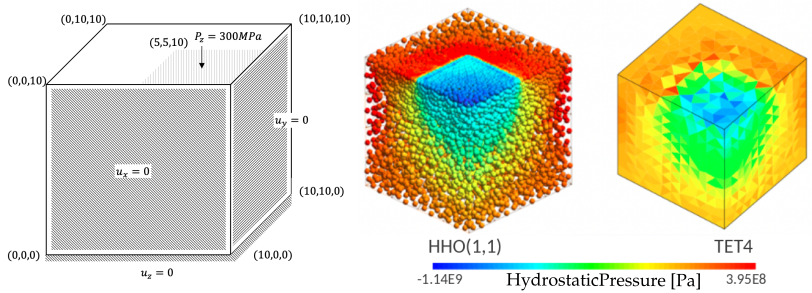
\includegraphics[width=12.cm]{../chapter_01_hho_mechanics/figures/cube.png}
    \caption{Hydrostatic pressure map one the reference configuration at the limit load}
    \label{fig_cube}
\end{figure}

% ---------------------------------------------------------
% PARAGRAPH
% ---------------------------------------------------------
\paragraph{Numerical results}

The pressure map at the end of the computation is displayed in Figure \ref{fig_cube}, and no sign of volumetric locking are present on the HHO computation, as opposed to the linear finite element one.
% ---------------------------------------------------------
% ---- SECTION
% ---------------------------------------------------------
\section{Reconstructed gradient and Elliptic projection}
\label{sec_appendix_gradient}

This section aims at generalizing the elliptic projection property of the reconstructed gradient, as introduced in \cite{di_pietro_hybrid_2015}. In the following, subspaces for the cell and faces approximations are not assumed to be polynomial necessarily.

Let $\displacementSpaceCell$ the space of cell kinematically admissible displacements, and $\displacementSpaceDCell$ that of face kinematically admissible displacements. The space for statically admissible stress and strain is denoted $\stressSpaceCell$.
%
%
%
Let $\discreteDisplacementSpaceCell \subset \displacementSpaceCell$ and $U^\perp(\cell) \subset \displacementSpaceCell$ such that $\displacementSpaceCell = \discreteDisplacementSpaceCell \oplus U^\perp(\cell)$, and set $\tensori{u}{}_{\cell} = \tensori{u}{}_{\cell}^h + \tensori{u}{}_{\cell}^\perp$ with
$\tensori{u}{}_{\cell}^h \in U^h(\cell)$ and $\tensori{u}{}_{\cell}^\perp \in U^\perp(\cell)$ the orthogonal projections of $\tensori{u}{}_{\cell}$ onto $U^h(\cell)$ and $U^\perp(\cell)$ respectively.
Let $V^h(\dCell) \subset \displacementSpaceDCell$ and $\tensori{u}{}_{\dCell}^h \in V^h(\dCell)$ the orthogonal projection of $\tensori{u}{}_{\cell}$ onto $V^h(\dCell)$.
The orthogonal projection of $\tensori{u}{}_{\cell}$ onto $U^h(\cell) \times V^h(\dCell)$ is then the displacement pair $(\tensori{u}{}_{\cell}^h, \tensori{u}{}_{\dCell}^h)$.
Let $S^h(\cell) = \{ \tensorii{\tau}{}_{\cell}^h \in \stressSpaceCell \ \ \vert \ \ \nabla \cdot  \tensorii{\tau}{}_{\cell}^h \in U^h(\cell) \ \ \vert \ \  \tensorii{\tau}{}_{\cell}^h \vert_{\dCell} \cdot \tensori{n}{} \in V^h(\dCell) \}$,
and $\tensorii{G}{}_{\cell}^h \in S^h(\cell)$ the solution of \eqref{eq_grad} for $(\tensori{u}{}_{\cell}^h, \tensori{u}{}_{\dCell}^h)$ such that
%
%
%
\begin{equation}
    \begin{aligned}
        \int_{\cell} \tensorii{G}{}_{\cell}^h(\tensori{u}{}_{\cell}^h, \tensori{u}{}_{\dCell}^h) : \tensorii{\tau}{}_{\cell}^h
        =
        \int_{\cell} \nabla \tensori{u}{}_{\cell}^h : \tensorii{\tau}{}_{\cell}^h
        +
        \int_{\dCell} (\tensori{u}{}_{\dCell}^h - \tensori{u}{}_{\cell}^h \vert_{\dCell}) \cdot \tensorii{\tau}{}_{\cell}^h \vert_{\dCell} \cdot \tensori{n}{}
        &&
        \ \ \ \ \ \ \ \ 
        &&
        \forall \tensorii{\tau}{}_{\cell}^h \in S^h(\cell)
    \end{aligned}
\end{equation}
%
%
%
using the fact that $\tensori{u}{}_{\dCell}^h$ is the projection of $\tensori{u}{}_{\cell}$ onto $V^h(\dCell)$ and that $\tensorii{\tau}{} \vert_{\dCell} \cdot \tensori{n}{} \in V^h(\dCell)$:
%
%
%
\begin{equation}
    \begin{aligned}
        \int_{\cell} \tensorii{G}{}_{\cell}^h(\tensori{u}{}_{\cell}^h, \tensori{u}{}_{\dCell}^h) : \tensorii{\tau}{}_{\cell}^h
        = &
        \int_{\cell} \nabla \tensori{u}{}_{\cell}^h : \tensorii{\tau}{}_{\cell}^h
        +
        \int_{\dCell} (\tensori{u}{}_{\cell} \vert_{\dCell} - \tensori{u}{}_{\cell}^h \vert_{\dCell}) \cdot \tensorii{\tau}{}_{\cell}^h \vert_{\dCell} \cdot \tensori{n}{}
        &&
        \ \ \ \ \ \ \ \ 
        &&
        \forall \tensorii{\tau}{}_{\cell}^h \in S^h(\cell)
        \\
        = &
        \int_{\cell} \nabla \tensori{u}{}_{\cell}^h : \tensorii{\tau}{}_{\cell}^h
        +
        \int_{\dCell} \tensori{u}{}_{\cell}^\perp \vert_{\dCell} \cdot \tensorii{\tau}{}_{\cell}^h \vert_{\dCell} \cdot \tensori{n}{}
        &&
        \ \ \ \ \ \ \ \ 
        &&
        \forall \tensorii{\tau}{}_{\cell}^h \in S^h(\cell)
    \end{aligned}
\end{equation}
%
%
%
using the divergence theorem and the fact that $\nabla \cdot  \tensorii{\tau}{}_{\cell}^h \in U^h(\cell)$, one has :
%
%
%
\begin{equation}
    \begin{aligned}
        \int_{\cell} \nabla \tensori{u}{}_{\cell}^\perp : \tensorii{\tau}{}_{\cell}^h
        =
        \int_{\dCell} \tensori{u}{}_{\cell}^\perp \vert_{\dCell} \cdot  \tensorii{\tau}{}_{\cell}^h \vert_{\dCell} \cdot \tensori{n}{}
        % &&
        % \ \ \ \ \ \ \ \ 
        % &&
        % \forall \tensorii{\tau}{}_{\cell}^h \in S^h(\cell)
    \end{aligned}
\end{equation}
%
%
%
such that :
%
%
%
\begin{equation}
    \begin{aligned}
        \int_{\cell} \tensorii{G}{}_{\cell}^h(\tensori{u}{}_{\cell}^h, \tensori{u}{}_{\dCell}^h) : \tensorii{\tau}{}_{\cell}^h
        = &
        \int_{\cell} \nabla \tensori{u}{}_{\cell}^h : \tensorii{\tau}{}_{\cell}^h
        +
        \int_{\cell} \nabla \tensori{u}{}_{\cell}^\perp : \tensorii{\tau}{}_{\cell}^h
        &&
        \ \ \ \ \ \ \ \ 
        &&
        \forall \tensorii{\tau}{}_{\cell}^h \in S^h(\cell)
        \\
        = &
        \int_{\cell} \nabla \tensori{u}{}_{\cell} : \tensorii{\tau}{}_{\cell}^h
        &&
        \ \ \ \ \ \ \ \ 
        &&
        \forall \tensorii{\tau}{}_{\cell}^h \in S^h(\cell)
    \end{aligned}
\end{equation}
%
%
%
which states that $\tensorii{G}{}_{\cell}^h(\tensori{u}{}_{\cell}^h, \tensori{u}{}_{\dCell}^h)$ is the orthogonal projection of $\nabla \tensori{u}{}_{\cell}$ onto $S^h(\cell)$.
By linearity of the algebraic trace operator, one has that $\text{Tr}(\tensorii{G}{}_{\cell}^h(\tensori{u}{}_{\cell}^h, \tensori{u}{}_{\dCell}^h))$ is the orthogonal projection of $\nabla \cdot \tensori{u}$, which proves robustness of the method
for linear elastic materials, since the Lamé coefficient $\lambda$ acts on $\nabla \cdot \tensori{u}$.

\bibliography{../bib_all}
\bibliographystyle{fr-insa}


\end{document}
